% Blockchain: Research and Applications (Elsevier/KeAi) submission
% Converted from IEEE Access source (accessBAK.tex) - format conversion only,
% scientific content preserved verbatim.
% =========================================================================

\PassOptionsToPackage{hyphens}{url}
\PassOptionsToPackage{hidelinks}{hyperref}

\documentclass[preprint,12pt]{elsarticle}

% ---------------------------------------------------------------------------
% Packages
% ---------------------------------------------------------------------------
\usepackage{silence}
\WarningFilter{caption}{Unknown document class}

\usepackage[utf8]{inputenc}
% NOTE: IEEE 'cite' package removed; elsarticle loads natbib (numbers) itself.
\usepackage{amsmath,amssymb,amsfonts}
\usepackage{algorithm}
\usepackage{algorithmic}
\usepackage{graphicx}
\usepackage{textcomp}
\usepackage{array}
\usepackage{tabularx}
\usepackage{xltabular}
\setlength{\LTcapwidth}{\textwidth}
\usepackage{booktabs}
\usepackage{ragged2e}
\usepackage{comment}
\usepackage{dblfloatfix}
\usepackage[caption=false]{subfig}
\usepackage{microtype}
\usepackage{xurl}
\usepackage{etoolbox}
\usepackage{listings}
\usepackage{xcolor}
\usepackage{needspace}
\usepackage{float}
\usepackage{placeins}
\usepackage{hyperref}

\graphicspath{{figures/}}

\newcommand{\workflowfigure}[2][]{%
  \includegraphics[width=\textwidth,height=0.34\textheight,keepaspectratio,#1]{#2}%
}

% ---------------------------------------------------------------------------
% Colors for listings
% ---------------------------------------------------------------------------
\definecolor{listingbg}{RGB}{248,248,248}
\definecolor{keywordblue}{RGB}{0,0,200}
\definecolor{commentgray}{RGB}{100,100,100}
\definecolor{stringteal}{RGB}{0,128,128}
\definecolor{linenumgray}{RGB}{150,150,150}
% ---------------------------------------------------------------------------
% Listing language definitions
% ---------------------------------------------------------------------------
\lstdefinelanguage{TypeScript}{
  language=Java,
  morekeywords={const,let,var,async,await,export,import,from,of,Promise,
                ArrayBuffer,Uint8Array,CryptoKey,string,boolean,number,
                void,undefined,null,true,false,as,type,interface,return},
  sensitive=true,
  morecomment=[l]{//},
  morestring=[b]',
  morestring=[b]"
}

% ---------------------------------------------------------------------------
% Global listing style
% ---------------------------------------------------------------------------
\lstset{
  basicstyle=\scriptsize\ttfamily,
  columns=fullflexible,
  keepspaces=true,
  breaklines=true,
  breakatwhitespace=true,
  postbreak=\mbox{\textcolor{commentgray}{\tiny$\hookrightarrow$}\space},
  frame=single,
  framesep=3pt,
  captionpos=t,
  belowcaptionskip=8pt,
  numbers=left,
  numberstyle=\tiny\color{linenumgray},
  numbersep=5pt,
  commentstyle=\color{commentgray}\itshape,
  keywordstyle=\color{keywordblue}\bfseries,
  stringstyle=\color{stringteal},
  showstringspaces=false,
  tabsize=2,
  backgroundcolor=\color{listingbg},
  xleftmargin=10pt,
  xrightmargin=0pt,
  aboveskip=6pt,
  belowskip=6pt,
  escapeinside={(*@}{@*)},
  literate={->}{{\textrightarrow}}1
           {=>}{{\ensuremath{\Rightarrow}}}1,
}

% ---------------------------------------------------------------------------
% Compact listing style (kept from IEEE source; still useful for long code)
% ---------------------------------------------------------------------------
\lstdefinestyle{tightcode}{
  basicstyle=\fontsize{6.6}{7.35}\selectfont\ttfamily,
  columns=fullflexible,
  keepspaces=true,
  breaklines=true,
  breakatwhitespace=true,
  postbreak=\mbox{\textcolor{commentgray}{\tiny$\hookrightarrow$}\space},
  frame=single,
  framesep=2.5pt,
  captionpos=t,
  belowcaptionskip=8pt,
  numbers=left,
  numberstyle=\tiny\color{linenumgray},
  numbersep=4pt,
  commentstyle=\color{commentgray}\itshape,
  keywordstyle=\color{keywordblue}\bfseries,
  stringstyle=\color{stringteal},
  showstringspaces=false,
  tabsize=2,
  backgroundcolor=\color{listingbg},
  xleftmargin=8pt,
  xrightmargin=0pt,
  aboveskip=4pt,
  belowskip=4pt,
  escapeinside={(*@}{@*)},
  literate={->}{{\textrightarrow}}1
           {=>}{{\ensuremath{\Rightarrow}}}1,
}

\journal{Blockchain: Research and Applications}

\begin{document}

\begin{frontmatter}

\title{A Secure and Auditable Framework for Legal Data Management:
A Hybrid Approach Using Hyperledger Fabric and IPFS}

\author[uiu]{Golam Bari Fardeen}
\author[uiu]{Namare Shakib Angkon}
\author[uiu]{Syed Zayan Anwar}
\author[uiu]{Md.\ Masum Mizi}
\author[uiu]{Shinthia Rahman}
\author[uiu]{Md.\ Motaharul Islam\corref{cor1}}
\ead{motaharul@cse.uiu.ac.bd}
\cortext[cor1]{Corresponding author.}

\affiliation[uiu]{organization={United International University},
            addressline={United City, Madani Avenue},
            city={Dhaka},
            postcode={1212},
            country={Bangladesh}}

\begin{abstract}
Legal document management systems typically centralize trust in privileged administrators, making it difficult for external parties to verify whether access decisions or audit records have been altered. This paper presents a hybrid legal-data management framework that places Hyperledger Fabric on the active document-release path rather than using it only as a passive audit log: every protected download must pass a Fabric chaincode access check before ciphertext or wrapped document keys are released. If Fabric is unavailable, the download path fails closed and returns a denial instead of falling back to a database access-control list. The framework combines browser-side encryption, encrypted off-chain storage in a private IPFS swarm, and on-chain anchoring of document hashes and content identifiers. In experimental evaluation, the REST-gateway workload sustains up to 193 transactions per second, exceeding the estimated baseline for a 1,000-user firm; Fabric-based access checks add no statistically significant delay over a database-only check; and outage simulations confirm that successful downloads drop to zero during Fabric unavailability, with service resuming automatically on reconnection. Prior permissioned-ledger document systems either anchor access decisions off the release path or price on-path authorization only for generic file sharing; none reports measured fail-closed behavior under ledger outage or the end-to-end cost of on-path enforcement against an audit-log-only baseline. The framework thus provides an empirical systems baseline for moving document-release decisions from application-only authorization to ledger-verifiable access-control state.
\end{abstract}

\begin{keyword}
Blockchain \sep Hyperledger Fabric \sep Legal document management \sep
Data integrity \sep Access control \sep Digital forensics
\end{keyword}

\end{frontmatter}

% =========================================================================
% SECTION I - INTRODUCTION
% =========================================================================
\section{Introduction}
\label{sec:introduction}

The legal industry depends on sensitive information. Law firms handle case
strategy, client communications, privileged records, and electronic evidence,
where confidentiality, integrity, and availability are essential. Yet many
legal document management systems still rely on centralized infrastructure
whose trust model has not kept pace with the threat landscape~\cite{aba2023,verizon2025}.

Recent sector evidence motivates this security concern. A 2024 NetDocuments
report found that more than half of identified data breaches at UK legal firms
were caused by insiders~\cite{ico2024trends}. The American Bar
Association's 2023 Legal Technology Survey also found that 29\% of respondents
answered yes to a security-breach question~\cite{aba2023}. These figures do
not prove that audit logs were altered. They do, however, motivate the
structural concern addressed here: NIST IR~8202~\cite{nistir8202} identifies
administrator control as a risk in permissioned systems, while NIST SP~800-92
\cite{nist800092} and NIST SP~800-53 AU-9 \cite{nist80053} emphasize protecting
audit logs against unauthorized modification.

The core problem is architectural. Conventional legal document management
systems centralize trust in a privileged database or application
administrator. That administrator, or an attacker who compromises their
credentials, may be able to read restricted documents, alter access-control
tables, modify audit logs, or erase evidence of having done so~\cite{nistir8202}.
A system may still encode a detailed role hierarchy, as illustrated in
Fig.~\ref{fig:rbac_hierarchy}. The central question is not whether such a
hierarchy can be represented in software, but whether its enforcement
decisions and audit records can be verified by parties other than the
administrator who recorded them.

\subsection{Existing Challenges and Problem Definition}
\label{sec:challenges}

Three deficiencies in current legal document management systems motivate this
work. First, audit trails are commonly stored in databases controlled by the
same organization whose behavior they are supposed to evidence. Append-only
database designs improve local tamper resistance. They do not provide
independently verifiable immutability if verification still depends on the
organization that controls the database~\cite{nistir8202}.

Second, access control is usually enforced through folder permissions,
application-layer role checks, or mutable ACL tables. A privileged
administrator may bypass or alter these controls directly. There is often no
verifiable record of when access was granted, under what conditions it was
meant to expire, or whether revocation was enforced~\cite{chainOfCustodySLR2023,cai2023timebound}.

Third, many systems record a username alongside an event without a
cryptographic signature binding the stated actor to the document content or
action being recorded. This leaves room for fabricated or misattributed
records~\cite{arora2019blockchain}.

These deficiencies share a root cause: the system's correctness depends on
administrative trust. In adversarial multi-firm legal workflows, documents may
be shared across firms, clients, experts, and regulators. Auditability
therefore requires more than a database log controlled by one party. The
required shift is from administrative trust to verifiable enforcement and
evidence: access decisions should be reproducible from policy state, audit
records should be independently checkable, and document integrity should be
anchored cryptographically.

\subsection{Proposed Solution and Research Objectives}
\label{sec:solution}

This paper proposes a hybrid legal document management framework in which
Hyperledger Fabric~\cite{androulaki2018hyperledger} is placed on the normal
authorization path, rather than used only as a passive audit log. Under normal
operation, a document download triggers a \texttt{CheckAccess} chaincode query.
The query evaluates time-bounded grant state and capability-token semantics
before the application releases ciphertext or a wrapped document key.

In this mode, the ledger does not merely record an application decision after
the fact. It provides the verifiable policy state against which the access
request is evaluated (cross-organization access; see
Section~\ref{sec:limitations} for intra-organization scope). When Fabric is
unavailable, the evaluated document-download path returns HTTP~503 and does
not fall back to a database ACL. Other Fabric-gateway paths follow the same
fail-closed pattern by design but were not independently outage-tested. This
prevents new document releases through the evaluated path during the tested
Fabric outage.

Encrypted document payloads are stored off-chain in a private two-node
InterPlanetary File System (IPFS) swarm~\cite{benet2014ipfs}. SHA-256 hashes
and content identifiers are anchored on-chain, keeping Fabric commit latency
independent of document size. The ordering service is a 3-node EtcdRaft
cluster distributed across FirmA, FirmB, and a regulator organization. This
provides crash-fault tolerance under Raft assumptions, not Byzantine
resistance to malicious orderer collusion~\cite{hyperledgerFabricOrderingService_v24,Ongaro2014}.

The framework design specifies browser-side AES-256-GCM encryption via the
WebCrypto API~\cite{fips197,w3cWebCrypto}. It also specifies an ECIES-style
P-256 hybrid wrapping construction, implemented with WebCrypto-supported
ECDH/KDF/AES-GCM primitives, for document-key wrapping. ECDSA P-256 document
signatures are generated by the user~\cite{fips1865}. The prototype implements
these mechanisms partially and discloses the remaining engineering gaps in
Table~\ref{tab:framework_vs_prototype}.

This work answers three research questions:

\begin{itemize}
\item \textbf{RQ1:} Can a permissioned blockchain architecture provide
ledger-verifiable access-control state to consortium peers under normal
operation, while enforcing a strict fail-closed policy for the evaluated
document-download path during Fabric unavailability?

\item \textbf{RQ2:} Does evaluating access control in chaincode at query time
impose acceptable read-latency overhead, and does absolute write latency remain
within the defined \textsc{SLO} for interactive legal workflows? We define
acceptable overhead as median read overhead below 50\,ms and total write
latency below 5\,s under realistic concurrency. The 50\,ms threshold follows
the cognitive heuristic that visual feedback under 100\,ms is perceived as
instantaneous~\cite{nielsen1993usability, miller1968response}. The 5.0\,s
write threshold is a conservative Service Level Objective (SLO) within the
10-second usability limit for background tasks before user context is
lost~\cite{nielsen1993usability}.

\item \textbf{RQ3:} Does the framework sustain throughput sufficient to absorb
realistic legal workload spikes? The evaluation uses a synthetic steady-state
baseline of a 1,000-user firm performing one document action per minute per
user (16.7\,TPS). This is an illustrative engineering assumption for capacity
planning, not a measured industry workload~\cite{aba2023,ilta2023}. Because
enterprise network traffic is bursty rather than uniform, a conservative
10$\times$ peak-load heuristic requires $\approx$167\,TPS. Section~\ref{sec:exp_sensitivity}
measures whether the tunable \texttt{BatchTimeout} configuration can reach
this peak-load target.

\end{itemize}

Throughout the paper, we distinguish between the \emph{proposed
framework}, which describes the intended security architecture, and
the \emph{prototype}, which is the measured implementation. The
prototype is useful for evaluating architectural viability and system
costs, but it is not presented as a production-ready legal platform.
Table~\ref{tab:framework_vs_prototype} summarizes the gap between
the complete framework design and the current implementation.

\subsection{Contributions}
\label{sec:contributions}


The primary contributions of this work are fourfold. First, the core
contribution is the measured relocation of the document-release
authorization boundary from application-only trust to ledger-verifiable
access-control state on the normal release path. The framework does not
propose a new access-control primitive, a Byzantine-fault-tolerant ordering
protocol, or a production-ready legal deployment. Fail-closed behavior is
empirically confirmed for the download path. Against the closest current
systems, the delta is measurement scope: RBAC-IPFS~\cite{liu2026rbacipfs}
prices on-path authorization for generic IPFS file sharing and zero-trust
delegation~\cite{mukta2026zerotrust} verifies capabilities on-ledger, but
no prior Fabric-and-IPFS document system reports measured fail-closed
behavior under ledger outage or quantifies the end-to-end premium of
on-path enforcement over the audit-log-only architecture it replaces.

Second, a proof-of-concept prototype is implemented and evaluated for a
three-organization legal consortium using Hyperledger Fabric, a
private two-node IPFS swarm, PostgreSQL operational storage, and a
Spring Boot REST gateway. The evaluation uses the REST-gateway
workload rather than an isolated peer/orderer microbenchmark, so the
reported throughput reflects the application path exercised by legal
document registration and retrieval.

Third, cryptographic mechanisms are integrated for document
confidentiality, key distribution, integrity anchoring, and user-level
signing. The framework uses AES-256-GCM for document encryption,
ECIES-style P-256 for per-recipient key wrapping, and ECDSA P-256 for
document signatures. Experiment~\hyperref[sec:exp_crypto]{6} shows that the main measured
advantage of ECIES in this setting is compact token size: 125 bytes
per recipient compared with 256 bytes for RSA-OAEP~2048, a
51.2\,\% reduction. Timing results are reported as Node.js WebCrypto
fallback measurements rather than browser-performance claims.

Fourth, an evidence-backed performance evaluation is provided. It covers
throughput, latency, file-size effects, audit-query cost, synthetic WAN
latency, \texttt{BatchTimeout} sensitivity, cryptographic operation cost,
ledger-history depth, and outage behavior. At the canonical
\texttt{BatchTimeout=2s} and \texttt{MaxMessageCount=500}, the REST-gateway
workload sustains approximately 68-70\,TPS, about 4.1 to 4.2$\times$ above the estimated
16.7\,TPS legal workload. Reducing \texttt{BatchTimeout} to 500\,ms produced
the highest measured throughput, 193.0\,TPS, for the evaluated
three-organization deployment.

Fabric \texttt{CheckAccess} latency is statistically indistinguishable from
the PostgreSQL-only ACL path after warm-up. Experiment~\hyperref[sec:exp_failclosed]{9}
(Fig.~\ref{fig:failclosed}) demonstrates strict fail-closed security
enforcement on the document-download path: successful downloads fall to
exactly zero for the full 45-second Fabric unavailability window
($t = 30$--$75$\,s), with HTTP\,503 denials sustained at 25--45 per second.
Normal operation resumes automatically after an approximately 15-second gRPC
reconnection lag.

The remainder of this paper is organized as follows.
Section~\ref{sec:literature_review} reviews related work.
Section~\ref{sec:system_arch} presents the system architecture.
Section~\ref{sec:governance_security} describes governance, security,
and the threat model. Section~\ref{sec:prototype_implementation}
details the prototype. Section~\ref{sec:performance} reports the
experiments. Section~\ref{sec:limitations} discusses limitations and
regulatory considerations. Section~\ref{sec:discussion} discusses the
research-question findings and interprets the experimental results.
Section~\ref{sec:conclusion} concludes the paper.

% Fig 1 - role hierarchy: single-column is appropriate (simple org-chart)
\begin{figure}[H]
\centering
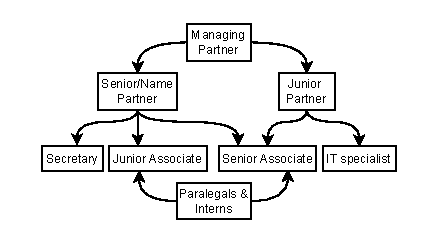
\includegraphics[width=\linewidth]{Hierarchy.pdf}
\caption{Role hierarchy enforced by the proposed framework, from
managing partners with full case visibility to paralegals
restricted to assigned documents only.}
\label{fig:rbac_hierarchy}
\end{figure}
\FloatBarrier

% =========================================================================
% SECTION II - LITERATURE REVIEW
% =========================================================================
% =========================================================================
% SECTION II - LITERATURE REVIEW
% =========================================================================
\section{Literature Review}
\label{sec:literature_review}

Blockchain applications in data management have expanded rapidly, evolving from integrity-preservation prototypes to systems that also address provenance, access control, and compliance
workflows~\cite{jaoude2019blockchain,casino2019systematic}. Two recent systematic reviews frame the specific problem addressed in this paper. Alkhatib \cite{alkhatib2022towards} reviewed blockchain-based identity and access management systems and found that independently verifiable audit trails and insider-aware access control remain open deployment challenges: many systems record access events after they occur, but still rely on a centralized application server or institutional database to decide whether an access request should be allowed. Precht et al.~\cite{paperlessEverything2025} similarly identify the absence of production-grade access-control enforcement in document management prototypes as a barrier to adoption. These reviews do not
imply that prior systems lack all access control; rather, they show
that the enforcement boundary often remains outside the ledger, so an
auditor must still trust the system that made the decision.
\begingroup
\scriptsize
\renewcommand{\arraystretch}{1.18}
\setlength{\tabcolsep}{4pt}
\begin{xltabular}{\textwidth}{@{}
>{\raggedright\arraybackslash}p{2.3cm}
>{\raggedright\arraybackslash}p{3.3cm}
>{\raggedright\arraybackslash}p{2.2cm}
c c c
>{\raggedright\arraybackslash}X
@{}}
\caption{Comparison with representative blockchain-based legal,
evidence-management, and access-controlled storage systems.
ACL = access-control decision evaluated on the normal document-release path;
Sig = user-level signature binding actor to document content;
Rev = ledger-verifiable revocation or expiry.
Y = supported; N = not supported; P = partial.}
\label{tab:literature_review}\\
\toprule
\textbf{System} &
\textbf{Primary contribution} &
\textbf{Tools} &
\textbf{ACL} &
\textbf{Sig} &
\textbf{Rev} &
\textbf{Main limitation relative to this work} \\
\midrule
\endfirsthead
\multicolumn{7}{@{}l}{\textit{Table \thetable\ (continued)}}\\
\toprule
\textbf{System} & \textbf{Primary contribution} & \textbf{Tools} &
\textbf{ACL} & \textbf{Sig} & \textbf{Rev} &
\textbf{Main limitation relative to this work} \\
\midrule
\endhead
\midrule
\endfoot
\bottomrule
\endlastfoot

Liu and Zheng~\cite{liu2024blockchain} &
Judicial evidence preservation with on-chain anchoring and off-chain storage. &
Blockchain + IPFS &
N & N & N &
Evidence integrity is anchored, but document access is not evaluated by ledger-visible policy before release. \\

Kim et al.~\cite{twoLevelBlockchain} &
Two-level evidence blockchain separating active and static investigation data. &
Two-level blockchain &
N & N & N &
Improves evidence lifecycle organization, but does not provide query-time document-level chaincode authorization. \\

Onyeashie et al.~\cite{onyeashie2025fabricEvidence} &
Multi-party evidence workflow using Fabric channels and IPFS storage. &
Fabric + IPFS &
N & N & N &
Supports workflow separation, but dynamic document ACL evaluation is not placed on every download path. \\

Verma et al.~\cite{verma2021nyaya} &
Tamper-evident judicial record management and timestamped action logging. &
Public blockchain &
N & N & N &
Provides timestamping and integrity evidence, but does not target confidential document retrieval or private access enforcement. \\

Hanafi et al.~\cite{hanafi2021ipfschain} &
Chain-of-custody auditing with Fabric and IPFS. &
Fabric + IPFS &
N & N & N &
Uses Fabric mainly for audit recording; per-request access enforcement and per-recipient key wrapping are not evaluated. \\

Guo et al.~\cite{guo2024efficient} &
Secure record storage and event auditing combining IPFS and Fabric. &
Fabric + IPFS &
N & N & N &
Uses Fabric mainly for audit recording; per-request access enforcement and per-recipient key wrapping are not evaluated. \\

Liu et al.~\cite{liu2026rbacipfs} &
Role-based access control for IPFS with root-CID smart-contract authorization on the retrieval path. &
Fabric + IPFS &
Y & N & Y &
Prices on-path authorization for generic file sharing (146--156\,ms end-to-end under 50\,ms emulated WAN), but does not evaluate ledger-outage behavior, an enforcement-cost baseline, per-recipient key wrapping, or a legal workflow. \\

Chen et al.~\cite{chen2022filewallet} &
Peer-to-peer personal and organizational file management on Fabric and IPFS. &
Fabric + IPFS &
P & N & N &
Chaincode privilege checks are validated functionally but never timed; no fail-closed design, expiry, or per-recipient key distribution. \\

Mukta et al.~\cite{mukta2026zerotrust} &
Zero-trust capability delegation with verifiable credentials on Fabric. &
Fabric + SSI &
P & P & Y &
Delegation verification is benchmarked as a chaincode operation (peak 29.4\,TPS), but there is no storage tier: authorization is never enforced on a document-release path. \\

Peelam et al.~\cite{peelam2026decentralized} &
NFT-based evidence registration with fog computing and IPFS. &
Ethereum + IPFS &
N & P & N &
Evidence minting and transfer delays are seconds-scale; document access is not evaluated by ledger-visible policy before release. \\

Notash et al.~\cite{notash2026adaptive} &
Adaptive access-control framework for e-health data sharing with broadcast encryption. &
Fabric + IPFS &
P & N & P &
Access policies are enforced and formally analyzed, but enforcement latency on the release path is not isolated (reported metrics are workflow-scale averages). \\

Capability and ABAC systems~\cite{macaroons2014,zanzibar2019,qian2021cpabe} &
Fine-grained delegation or attribute-based authorization. &
Capability / ABAC &
P & N & Y &
Policies can be expressive, but enforcement authority is typically a service layer rather than consortium-visible ledger state. \\

Proposed framework and prototype &
Ledger-verifiable legal document authorization with encrypted off-chain storage. &
Fabric + IPFS &
Y & P & Y &
Strict access uses Fabric fail-closed; prototype limits include custodial Fabric identities, custodial transaction attribution for user-level signatures, and 2-node IPFS swarm. \\

\end{xltabular}
\endgroup


Table~\ref{tab:literature_review} compares prior systems based on
where the access decision is made. The table does not imply that prior
systems lack access control entirely. Instead, it distinguishes systems
where access is mainly decided by the application server from systems
where the decision is evaluated against ledger-visible policy before a
document is released. The proposed contribution is therefore not a new
access-control primitive, but a shift in the enforcement boundary: in
normal operation, document access is checked through Fabric chaincode
before protected material is returned to the user.

\subsection{Foundational Technologies}
\label{sec:foundations}

Hyperledger Fabric is a permissioned blockchain platform in which
participants are authenticated through Membership Service Providers
(MSPs) that issue X.509 identities. Fabric supports configurable
endorsement policies, private data collections, and channel-level
governance, making it suitable for consortia of known institutions
that require verifiable execution without exposing all data to a
public network~\cite{androulaki2018hyperledger,fabricMSP,
fabricPDCDoc,fabricEndorsementDoc}. These properties are relevant to
legal workflows because firms, clients, experts, and regulators often
need shared evidence of actions without merging their internal
databases.

Fabric is not designed to store large binary documents directly on the
ledger. For that reason, many systems pair Fabric or another
blockchain with IPFS~\cite{benet2014ipfs}. IPFS provides
content-addressed storage: if a stored object changes, its content
identifier changes, making tampering detectable by address mismatch.
However, content addressing does not by itself guarantee availability.
Objects must be pinned and replicated by designated nodes, and private
deployments require governance over who pins, who can fetch, and how
long content is retained~\cite{ipfsDocsQuickstartPin2025,
ipfsDocsKuboGarbageCollection}. The proposed framework therefore uses
IPFS only for encrypted off-chain payload storage, while Fabric stores
the verifiable metadata needed for integrity and access-control
auditing.

Chaincode (Hyperledger Fabric uses the terms \emph{chaincode}
and \emph{smart contract} interchangeably; this paper uses
\emph{chaincode} throughout) can automate policy decisions, but the security
benefit depends on where the policy is evaluated. If chaincode only
records an event after an application server has already made the
access decision, the blockchain improves auditability but does not
remove the application server from the authorization trust boundary.
The distinction used in this paper is narrower: the proposed framework
places a chaincode query on the normal document-download path so that
the access decision is evaluated against ledger state before the
application releases the protected material.

\subsection{Evolution of Blockchain in Legal Technology}
\label{sec:evolution}

\subsubsection{Integrity-Only Systems}

Early legal and forensic blockchain systems focused primarily on
tamper-evident chain of custody. NyaYa~\cite{verma2021nyaya} anchors
judicial records to establish timestamped evidence integrity, while
Forensic-chain~\cite{lone2019forensic} and Block4Forensic
\cite{cebe2018block} apply similar ideas to digital-forensics and IoT
evidence pipelines. These systems demonstrate the value of immutable
timestamps and hash anchoring, but they generally treat access control
as an external concern. In other words, the ledger can help prove that
a record existed at a given time, but it does not necessarily decide
who may retrieve a confidential document in a multi-party legal
workflow.

\subsubsection{Hybrid Blockchain--IPFS Storage Systems}

A second line of work combines blockchain anchoring with off-chain
storage to address scalability. Liu and Zheng~\cite{liu2024blockchain}
and Jlil et al.~\cite{jlil2024blockchain} show that legal or criminal
records can be represented by on-chain hashes while the larger payload
is stored elsewhere. This pattern is useful because it avoids placing
large documents directly on-chain. Its limitation is that storage
integrity and access authorization are different problems. A document
hash can prove that a retrieved payload matches a prior record, but it
does not by itself enforce time-bounded sharing, revocation, or
per-recipient key distribution.

\subsubsection{Multi-Party and Fabric-Based Evidence Systems}

More recent systems use permissioned blockchains to support
multi-institution evidence workflows. Kim et al.~\cite{twoLevelBlockchain}
organize evidence across active and static chains, and Onyeashie
et al.~\cite{onyeashie2025fabricEvidence} use Fabric and IPFS to separate law-enforcement, forensic, and judicial workflows. Hanafi et al.~\cite{hanafi2021ipfschain} and Guo et al. \cite{guo2024efficient} also combine IPFS and Fabric for secure record storage and event auditing, demonstrating the architecture's viability for highly confidential, role-based document sharing. These systems move closer to the legal-consortium model considered in this paper, but their
primary contribution remains evidence management and audit recording. To the best of the authors' knowledge, none of the prior legal and evidence-management systems in Table~\ref{tab:literature_review} report evaluating an access-control decision against chaincode on the critical path of every document download or measuring the latency cost of doing so in a REST-gateway legal-document workflow, leaving an open baseline against which future permissioned-blockchain document-access systems can calibrate their access-control overhead.

\subsubsection{Access-Control-Centric Fabric and IPFS Systems}

A fourth line of work makes the access decision itself the primary
contribution. FileWallet~\cite{chen2022filewallet} manages personal and
organizational files on Fabric and IPFS with chaincode privilege checks,
but validates them functionally rather than measuring their cost, and
provides neither expiry nor per-recipient key distribution. Mukta et
al.~\cite{mukta2026zerotrust} verify zero-trust capability delegations
on Fabric and benchmark the delegation chaincode with Hyperledger
Caliper, but the architecture has no storage tier: no document release
is ever gated by the verified capability. Notash et
al.~\cite{notash2026adaptive} enforce adaptive policies for e-health
sharing over Fabric and IPFS and analyze them formally, reporting
workflow-scale averages rather than isolating the enforcement decision
on the release path. Closest to this work, the recent RBAC-IPFS scheme
of Liu et al.~\cite{liu2026rbacipfs} performs a single root-CID
smart-contract authorization on the IPFS retrieval path and, notably,
\emph{does} measure it: contract execution in 1--2\,ms and 146--156\,ms
end-to-end retrieval under an emulated 50\,ms wide-area network. That
system targets generic file sharing; what remains unmeasured in it, and
in all of the systems above, is the behavior of the enforcement point
when the ledger is unavailable, the end-to-end premium of on-path
enforcement relative to the audit-log-only architecture it replaces,
and the domain mechanisms a legal consortium requires (time-bounded
grants, per-recipient key wrapping, user-level signature binding, and a
regulator role).

\subsection{Identified Research Gaps}
\label{sec:gaps}

The reviewed literature reveals four gaps that motivate the proposed
framework. First, most blockchain-based evidence systems provide
tamper-evident storage or timestamping but leave authorization to the
application layer: Liu and Zheng~\cite{liu2024blockchain}, Hanafi et
al.~\cite{hanafi2021ipfschain}, and Guo et al.~\cite{guo2024efficient}
anchor or audit access events without evaluating the decision against
ledger state before release, so a compromised or overly privileged
application server may still authorize access using state that is not
independently verifiable at the time of access. RBAC-IPFS
\cite{liu2026rbacipfs} closes part of this gap for generic file sharing
by pricing an on-path authorization, but reports neither
ledger-outage behavior nor the cost of on-path enforcement relative to
an audit-log-only baseline. Second, access-control models are often
coarse-grained or static: capability delegation is verified on-ledger
without gating any storage tier~\cite{mukta2026zerotrust}, and
file-management ACLs lack expiry and revocation
semantics~\cite{chen2022filewallet}, whereas legal collaboration
requires operation-specific capabilities, expiry, revocation, and
auditable sharing across institutions. Third, user-level
non-repudiation is often incomplete: a ledger transaction may show
that an organization submitted an event, but not that a specific user
signed the document content or action being
recorded~\cite{peelam2026decentralized}. Fourth, off-chain storage
availability is frequently assumed rather than governed; IPFS content
must be pinned and replicated deliberately.

The proposed framework addresses these gaps by moving the enforcement boundary onto the normal document-release path.
The contribution is not a new access-control primitive, not a
Byzantine-fault-tolerant ordering protocol, and not a
production-ready legal deployment: it is a measured relocation of
the document-release authorization boundary from application-only
trust to ledger-verifiable access-control state on the
normal release path, with fail-closed behavior empirically
confirmed for the download path. The prototype still has limitations, including custodial Fabric
identity handling and \texttt{localStorage}-based key storage, and
those limitations are disclosed in
Section~\ref{sec:prototype_implementation} and
Section~\ref{sec:limitations}.

Two related paradigms help clarify the boundary of the contribution.
Capability systems such as Macaroons~\cite{macaroons2014} and
large-scale authorization systems such as Zanzibar~\cite{zanzibar2019}
support expressive delegation and centralized policy evaluation at
scale. The proposed framework does not replace those systems or claim
to improve their policy expressiveness. Its difference is the audit
and trust model: in the normal path, the policy state used for access
evaluation is visible to consortium peers through Fabric rather than being
only an internal service decision. Attribute-Based Access Control
(ABAC)~\cite{hu2014guide}, including blockchain-assisted ABAC proposals such
as Waheed et al.~\cite{waheed2025dynamicabac}, can express fine-grained
conditions. The present work is complementary: it focuses on where the
decision is enforced and audited in a legal-document workflow, and on
the measured overhead of placing that decision on the Fabric-backed
access path.

Table~\ref{tab:arch_comparison} summarizes how the proposed
architecture differs from these design classes across the
properties most relevant to legal consortium deployments.

\begingroup
\footnotesize
\renewcommand{\arraystretch}{1.18}
\setlength{\tabcolsep}{4pt}
\begin{xltabular}{\textwidth}{|>{\RaggedRight\arraybackslash}p{3.05cm}|>{\RaggedRight\arraybackslash}X|>{\RaggedRight\arraybackslash}X|>{\RaggedRight\arraybackslash}X|>{\RaggedRight\arraybackslash}X|}
\caption{Architectural Comparison of Access-Control Designs.
This table compares the authorization trust boundary across four
design classes. The centralized and append-only DB baselines are operational latency references, not security-equivalent alternatives.}
\label{tab:arch_comparison}\\
\hline
\textbf{Property} &
\textbf{centralized DB} &
\textbf{Append-only DB} &
\textbf{Fabric audit-only} &
\textbf{This work} \\
\hline
\endfirsthead
\multicolumn{5}{l}{\textit{Table \thetable\ (continued)}}\\
\hline
\textbf{Property} &
\textbf{centralized DB} &
\textbf{Append-only DB} &
\textbf{Fabric audit-only} &
\textbf{This work} \\
\hline
\endhead
\hline
\endfoot
\endlastfoot
Admin can silently alter access log &
Yes &
Hard &
No (Fabric ledger; operational PostgreSQL log excluded) &
No \\
\hline
Per-request ledger authorization on document-release path &
No &
No &
No &
Yes \\
\hline
Fail-closed on outage &
No &
No &
No &
Yes (empirically validated on document-download path; other paths fail-closed by design) \\
\hline
Ciphertext integrity verifiable by client &
No &
No &
Partial &
Yes ($\mathcal{H}_D$ anchored on-chain) \\
\hline
On-chain metadata leakage &
None &
None &
Medium &
Medium (encrypted content is protected, but ledger metadata and access patterns
remain visible to channel members. PDC-based reduction is future hardening.) \\
\hline
Per-user transaction attribution &
Yes &
Yes &
Custodial (prototype) &
Custodial (prototype); per-user X.509 is production path \\
\hline
Byzantine-fault-tolerant ordering &
N/A &
N/A &
No (CFT) &
No (CFT); documented SmartBFT production path~\cite{fabricWhatsNew3x,fabricOrderingServiceLatest} \\
\hline
Production-ready &
Yes &
Yes &
Partial &
No (proof-of-concept prototype) \\
\hline
\end{xltabular}
\endgroup

% SECTION III - SYSTEM ARCHITECTURE
% =========================================================================
\section{System Architecture and Design}
\label{sec:system_arch}

The proposed framework separates three cryptographically distinct
concerns: document confidentiality (AES-256-GCM client-side
encryption), access policy enforcement (chaincode-authoritative ACL),
and audit integrity (dual-store: Fabric ledger and PostgreSQL
append-only log). This section describes the operational workflows,
the cryptographic layer, the two-layer access control architecture,
and the audit architecture. Governance, consensus, and the formal
threat model are in Section~\ref{sec:governance_security}.

\subsection{Operational Workflows}
\label{sec:workflows}

\subsubsection{User Registration}
Fig.~\ref{fig:user_registration} shows the registration workflow.
The user submits identity attributes; the application server creates
a profile in the off-chain PostgreSQL identity database and enrolls
the user with the Fabric CA, issuing an X.509 certificate under the
organization's MSP~\cite{fabricCADoc,fabricMSP}. In the framework
design, each user also generates two keypairs in the browser at
registration: an ECIES-style P-256 keypair ($sk_{ecies}$, $pk_{ecies}$)
for document key wrapping and an ECDSA~P-256 keypair ($sk_{sign}$,
$pk_{sign}$) for document signing (Section~\ref{sec:crypto}). The
two keypairs are intentionally distinct so that a key used for
encryption is never used for signing, following key-separation
practice~\cite{nist800131a}. In the measured prototype, Fabric transaction submission is performed
through server-managed MSP credentials rather than per-user Fabric
certificates; per-user X.509 enrollment is the production path.

% Fig 2 - complex multi-swimlane diagram: two-column
\begin{figure*}[!t]
    \centering
    \workflowfigure{user_registration_flow.pdf}
    \caption{User registration workflow: browser-side P-256 keypair
    generation, PBKDF2-wrapped key storage in \texttt{localStorage},
    public-key registration, and Fabric CA enrollment.}
    \label{fig:user_registration}
\end{figure*}

\subsubsection{Document Upload and Registration}
Fig.~\ref{fig:document_upload} illustrates the upload workflow. The
browser first generates a fresh AES-256-GCM document key $k_{enc}$ and a
96-bit IV using \texttt{window.crypto.getRandomValues}. It computes the
SHA-256 plaintext hash $\mathcal{H}_D$ \emph{before} encryption so that
$\mathcal{H}_D$ can serve as the document-integrity anchor.

After encryption, the browser prepends the IV to form the stored payload
$D_{store} = IV \| D_{enc}$ and computes
$\mathcal{H}_C = \text{SHA-256}(D_{store})$. This hash covers exactly
the byte sequence from which the IPFS CID is derived. Strict client-side
encryption ensures that the server receives only the IV-prepended
ciphertext, not plaintext.

The signing key $sk_{sign}$ then signs
$\mathcal{H}_D \| \mathcal{H}_C \| \texttt{UTF-8}(id_D)$. This avoids a
second round-trip for the CID while still binding the user to the exact
plaintext content, the exact IPFS storage payload, and the document
identifier. Because $\mathcal{H}_C$ hashes $IV \| D_{enc}$, any later
attempt to swap the IPFS ciphertext invalidates the signature.

After IPFS returns the CID, the server invokes the \texttt{RegisterDocument}
chaincode with $\mathcal{H}_D$, the CID, metadata, and $\sigma$. The
prototype signature does not bind upload timestamp or owner metadata;
that binding is a production hardening item~\cite{fips1865}. Fabric
transaction-level non-repudiation also remains custodial because the
prototype submits transactions through server-managed MSP credentials
(Section~\ref{sec:prototype_scope}).


\begin{figure*}[!t]
    \centering
    \workflowfigure[width=0.86\textwidth]{document_upload_flow.pdf}
    \caption{Document upload and on-chain registration, showing browser-side $k_{enc}$ generation, plaintext hashing before encryption, sign-then-store ordering, IPFS upload, and CID anchoring.}
    \label{fig:document_upload}
\end{figure*}

\subsubsection{Access Control and Document Retrieval}
Access control is enforced in two layers. Fig.~\ref{fig:access_control}
shows Layer~1: Spring Security JWT RBAC validates the caller's role
before the method body executes. Fig.~\ref{fig:document_retrieval}
shows Layer~2: the \texttt{CheckAccess} chaincode evaluates the on-chain
ACL at query time. Only if both layers authorize the request does the
server retrieve the ciphertext from IPFS and the ECIES-wrapped key token
from ledger storage. The client unwraps $k_{enc}$ using $sk_{ecies}$ and
decrypts locally.

On the evaluated document-download path, Fabric unavailability causes
HTTP~503 denial and no database ACL fallback. Other Fabric-gateway paths
follow the same fail-closed pattern by design but were not independently
outage-tested. The service records a \texttt{FABRIC\_OUTAGE\_ACCESS\_DENIED}
event in the operational \mbox{PostgreSQL} audit log. Because Fabric is unavailable at the time of denial, these outage events are not
synchronously committed to the ledger and therefore inherit
operational-log trust limits rather than ledger-verifiability guarantees.
This prevents new document releases during the tested Fabric outage and
prevents bypass of the chaincode authority~\cite{RBACSandhu,androulaki2018hyperledger}.


\begin{figure*}[!tbp]
    \centering
    \workflowfigure[width=0.72\textwidth]{access_control_flow.pdf}
    \caption{Layer~1 access control: Spring Security JWT RBAC at the
    API gateway. Requests failing role validation are rejected before
    reaching the blockchain layer.}
    \label{fig:access_control}
\end{figure*}

\begin{figure*}[!tbp]
    \centering
    \workflowfigure[width=0.72\textwidth]{document_retrieval_flow.pdf}
    \caption{Layer 2 access control and document retrieval: \texttt{CheckAccess}
chaincode evaluates the on-chain ACL at query time. The client decrypts
locally; the server handles only ciphertext and ECIES-wrapped key tokens
stored as encrypted ledger/world-state values.}
    \label{fig:document_retrieval}
\end{figure*}

\subsubsection{Audit and Integrity Verification}
The system records every security-relevant action to two independent
stores: the Fabric ledger and the PostgreSQL \texttt{audit\_log}
table. Fabric is the independently verifiable record because any
consortium peer can query and validate ledger history. PostgreSQL is
the operational audit index, configured as INSERT-only by triggers and
used for low-latency dashboard queries. The two stores provide
different trust guarantees: PostgreSQL improves operational
visibility, while Fabric provides the stronger evidence against a
malicious or compromised database administrator. Figs.~\ref{fig:audit_trail}
and~\ref{fig:integrity_check} show the audit query and hash
verification workflows.

\begin{figure*}[!tbp]
    \centering
    \workflowfigure[width=0.74\textwidth]{audit_trail_flow.pdf}
    \caption{Audit trail retrieval. \texttt{GetHistoryForKey}
    returns the full transaction history for a document key and is
    independently verifiable by any consortium peer without trusting
    the application server.}
    \label{fig:audit_trail}
\end{figure*}

\begin{figure}[!t]
    \centering
    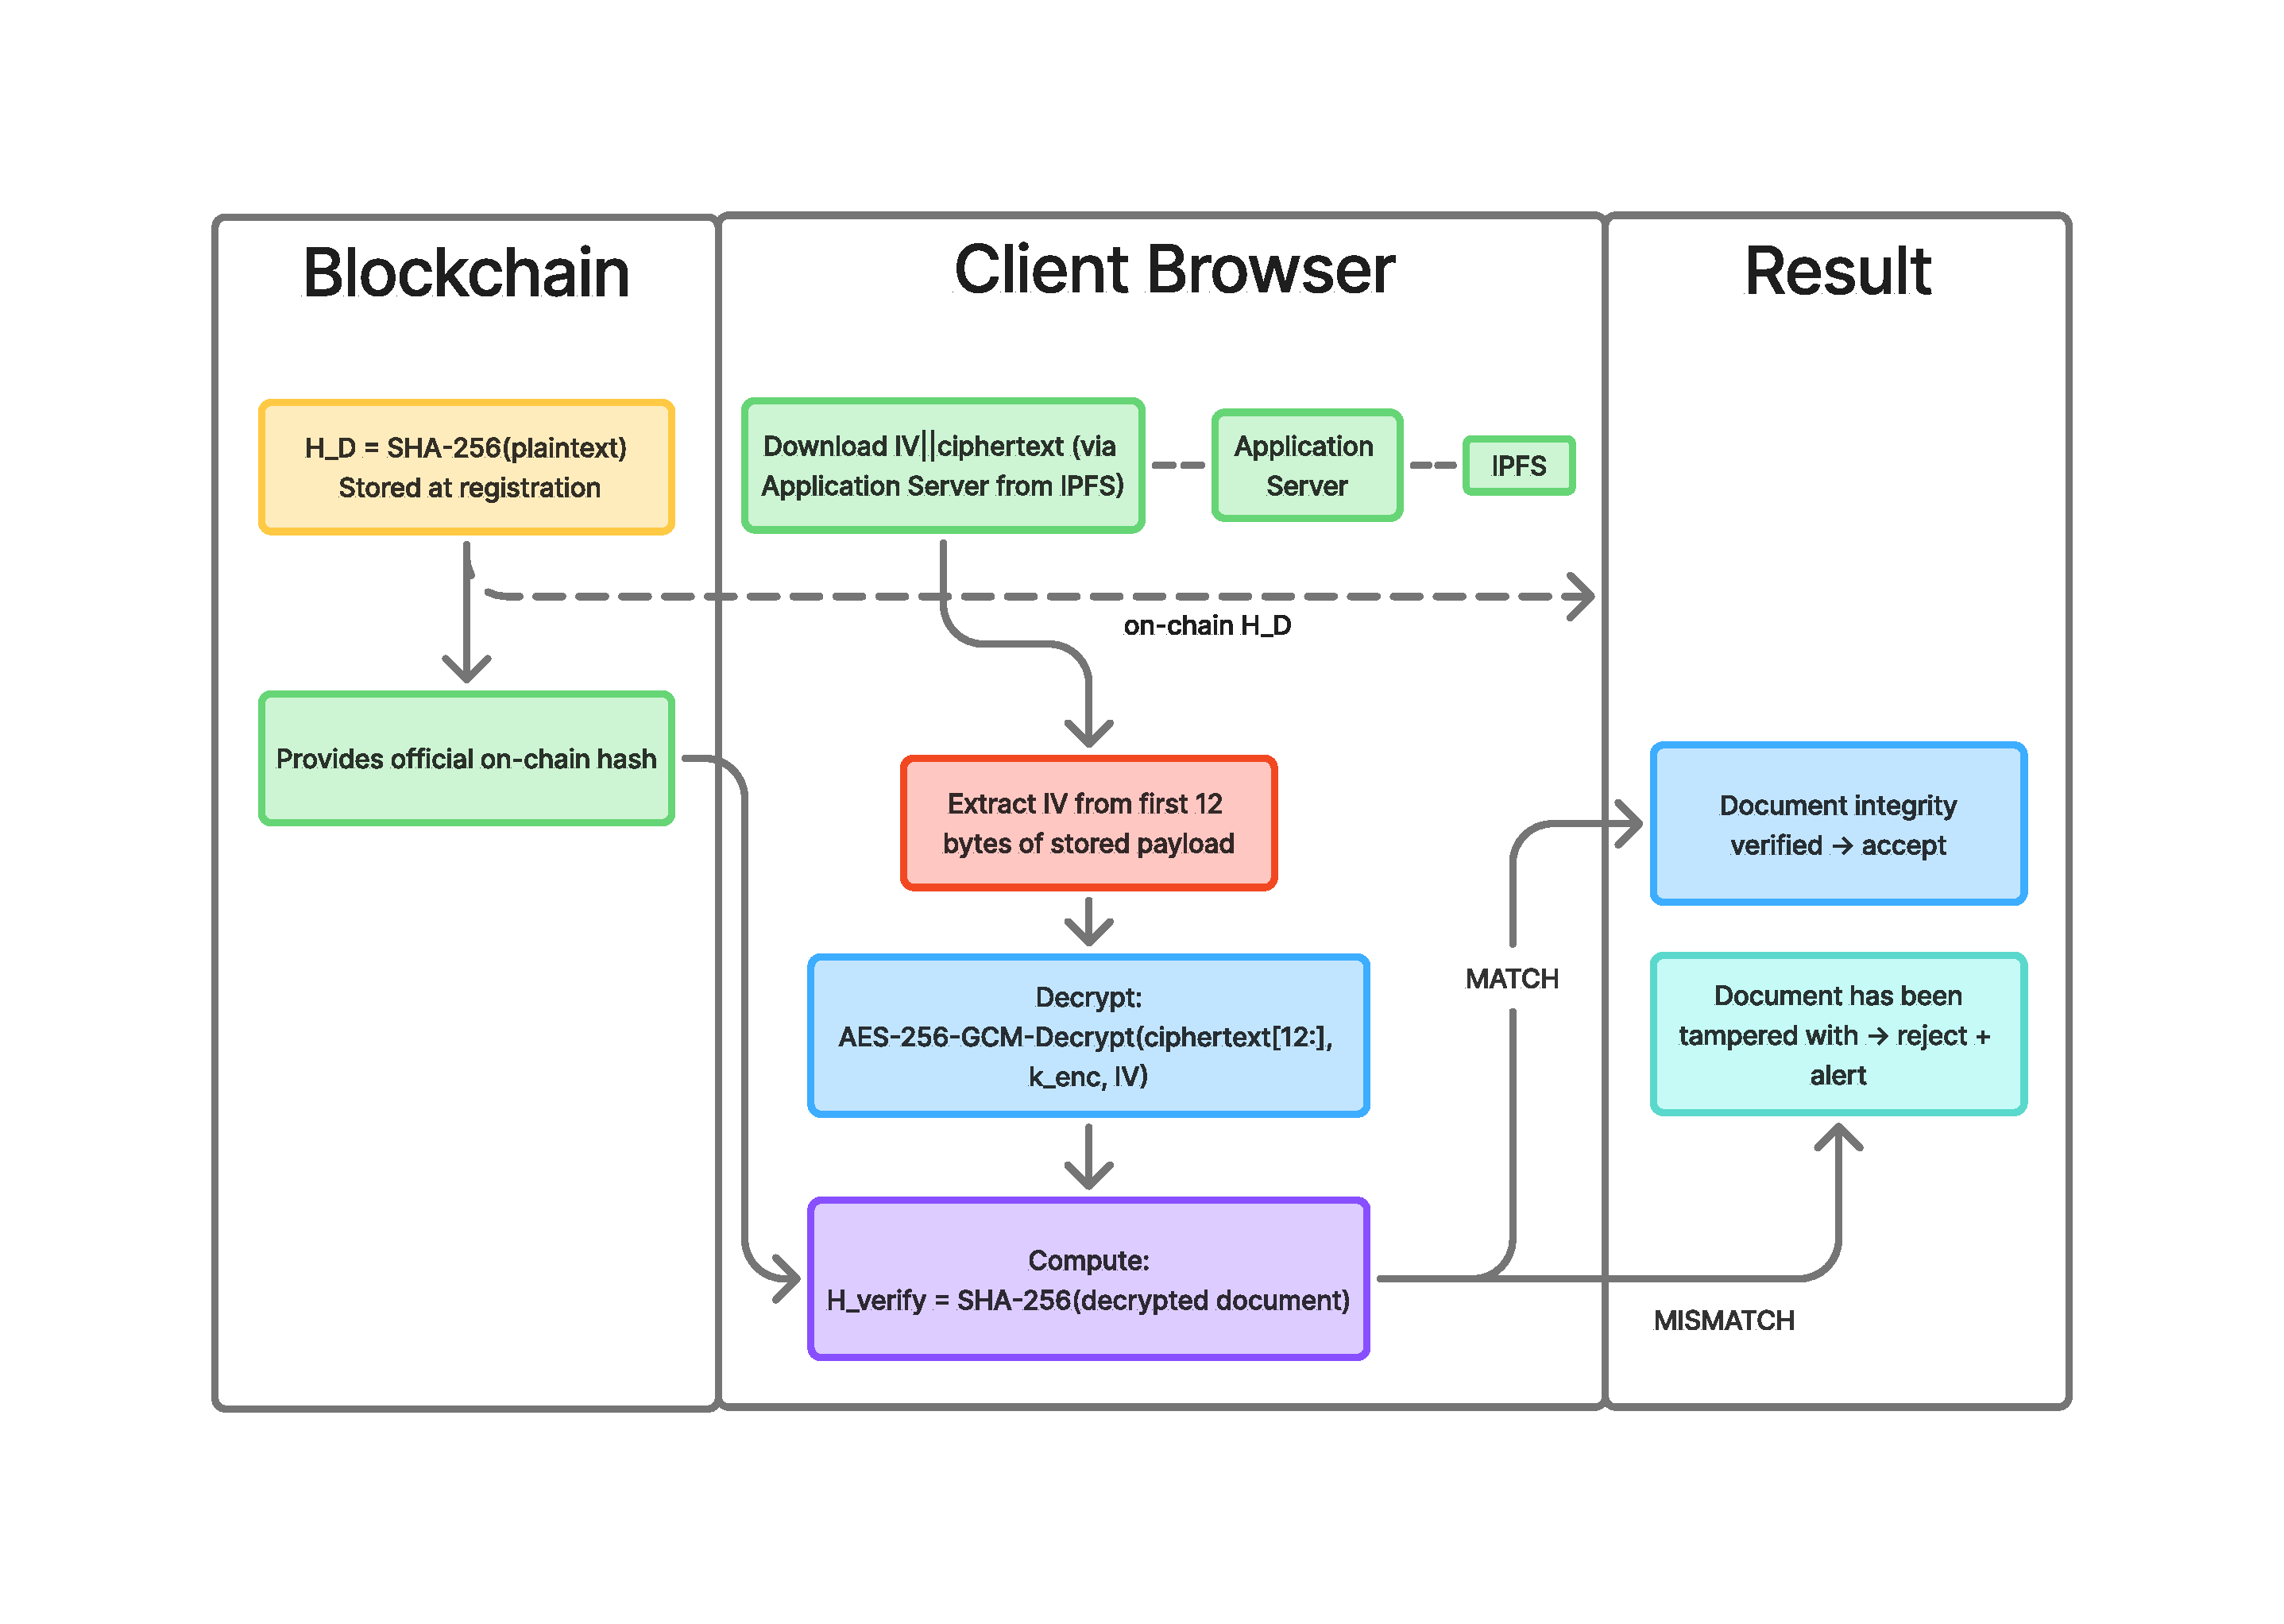
\includegraphics[width=\columnwidth]{integrity_check_flow.pdf}
    \caption{Document integrity verification by comparing on-chain $\mathcal{H}_D$ with the SHA-256 hash of the locally decrypted document.}
    \label{fig:integrity_check}
\end{figure}

\subsection{Cryptographic Layer}
\label{sec:crypto}

The framework uses a three-tier hybrid cryptographic design.
Symmetric encryption (AES-256-GCM) protects document content.
Asymmetric key wrapping using the Elliptic Curve Integrated Encryption
Scheme (ECIES) over P-256 distributes document keys to
authorized recipients. Digital signatures (ECDSA~P-256) bind each
document action to the acting user's identity. Fabric MSP
infrastructure uses ECDSA~P-256 for transaction signing
independently~\cite{fabricMSP,fips1865}. In the measured prototype, user-level document signatures and Fabric
transaction identity should therefore be interpreted separately because
Fabric transactions are submitted through server-managed MSP
credentials.

\subsubsection{Notation}

\begin{table}[ht]
    \caption{Notation}
    \centering
    \renewcommand{\arraystretch}{1.3}
    \begin{tabularx}{\columnwidth}{@{} p{2.2cm}
                                       >{\raggedright\arraybackslash}X @{}}
        \toprule
        \textbf{Symbol} & \textbf{Description} \\
        \midrule
        $D,\,M,\,U$ & Document, Metadata, User \\
        $sk,\,pk$ & Private and public key \\
        $k_{enc}$ & Per-document AES-256-GCM symmetric key \\
        $sk_{ecies},\,pk_{ecies}$ & ECIES-style P-256 keypair for key wrapping \\
        $sk_{sign},\,pk_{sign}$ & ECDSA P-256 keypair for signing \\
        $\mathcal{H}(\cdot)$ & SHA-256 hash function \\
        $\mathcal{H}_D$ & SHA-256 hash of plaintext
        document (plaintext hash; integrity anchor) \\
        $\mathcal{H}_C$ &
        SHA-256 hash of the IV-prepended ciphertext payload,
        $\mathcal{H}_C = \text{SHA-256}(IV \| D_{enc})$;
        covers the exact byte sequence stored in IPFS \\
        $\sigma$ & ECDSA P-256 digital signature \\
        $M_{pre}$ & Prototype signing payload component:
        $\texttt{UTF-8}(id_D)$ only. Framework design goal:
        deterministically serialized full metadata
        $\{id_D, \text{owner}, \text{filename}, t_{\text{now}}\}$;
        deferred to future work. \\
        $\|$ & Concatenation \\
        $\perp$ & Failure or null return \\
        \bottomrule
    \end{tabularx}
\end{table}

Algorithm~\ref{alg:doc_registration} formalizes the registration
process using the sign-then-store pattern: in the prototype, $\sigma$ is
computed over $\mathcal{H}_D \| \mathcal{H}_C \| \texttt{UTF-8}(id_D)$
before the IPFS upload, avoiding the circular dependency of signing a
value not yet known. The CID is submitted alongside $\sigma$ in the Fabric
transaction; any party verifying non-repudiation verifies $\sigma$ over
$\mathcal{H}_D \| \mathcal{H}_C \| \texttt{UTF-8}(id_D)$. With 96-bit IVs generated via a
CSPRNG and a fresh AES-256-GCM key per document (Algorithm~1,
lines~1--2), the birthday-bound IV collision probability for any
single key is negligible below $2^{32}$ documents
($<2^{-32}$ per NIST SP~800-38D~\cite{nist80038d}); per-document
key generation eliminates cross-document IV-reuse risk entirely: because
each document uses an independent $k_{enc}$, an IV collision in one
document has no cryptographic effect on any other document~\cite{nist80038d}.
Listing~\ref{lst:encrypt} (Appendix~\ref{app:listings}) shows the browser implementation.

\textbf{Protocol composition security.} The ECIES-style key-wrapping construction is
\emph{intended} to achieve \textsc{IND-CCA2} security under the Gap
Diffie-Hellman (\textsc{GDH}) assumption following Shoup's formal
model~\cite{shoup2001ecies,ieee1363a2004}; however, the prototype composes
\mbox{ECDH}, \mbox{HKDF-SHA-256}, and \mbox{AES-256-GCM} via WebCrypto
without a named ECIES primitive, and the formal \textsc{IND-CCA2} reduction
for this specific composition is left as future work.
Table~\ref{tab:eciestoken} defines the 125-byte token format used in the
prototype.

\begin{table}[ht]
\caption{ECIES-Style 125-Byte Wrapped-Key Token Format.\label{tab:eciestoken}}
\centering
\small
\begin{tabular}{llr}
\hline
Field & Content & Bytes \\
\hline
Ephemeral public key & Uncompressed P-256 point & 65 \\
AES-GCM nonce & 96-bit random IV & 12 \\
Wrapped key ciphertext & AES-256-GCM encrypted $k_{enc}$ & 32 \\
Authentication tag & AES-256-GCM tag & 16 \\
\hline
\textbf{Total} & & \textbf{125} \\
\hline
\end{tabular}
\vspace{2pt}
\footnotesize\parbox{\columnwidth}{KDF: HKDF-SHA-256 over the ECDH shared secret. AAD: empty in the prototype; binding the recipient public key as AAD is a production hardening item.}
\end{table}
%
\textsc{ECDSA}~P-256 achieves \textsc{EUF-CMA} under the elliptic curve discrete logarithm (\textsc{ECDLP}) assumption~\cite{fips1865}. In this setting, an adversary cannot forge a valid signature without the signing key.

The registration workflow uses a sign-then-store ordering. Before the IPFS upload, $\sigma$ is computed over three values: the 32-byte plaintext hash ($\mathcal{H}_D$), the 32-byte IV-prepended ciphertext-payload hash ($\mathcal{H}_C = \text{SHA-256}(IV \| D_{enc})$), and $\texttt{UTF-8}(id_D)$. This ordering avoids a circular dependency: the CID is not known until after upload, so signing a payload that includes the CID would require either a second round-trip or a separate commitment scheme.

Signing $\mathcal{H}_C$ still commits the user to the exact IPFS storage payload, including the prepended IV from which the CID is derived. An attacker therefore cannot swap the stored ciphertext later without invalidating the signature. The resulting construction binds both plaintext and ciphertext hashes, which is stronger than signing only plaintext while preserving the non-repudiation property of plaintext signing~\cite{fips1865,ieee1363a2004}.

The prototype relies on standard assumptions for ECIES-style wrapping, AES-GCM encryption, and ECDSA signatures, but it does not claim a new formal reduction for their exact WebCrypto composition. ECIES protects $k_{enc}$ in transit~\cite{ieee1363a2004}; AES-GCM protects document content at rest~\cite{fips197}; and ECDSA provides the user-key binding~\cite{fips1865}.

\begin{algorithm}[H]
\caption{Document Registration (Sign-Then-Store Pattern)}
\label{alg:doc_registration}
\small
\begin{algorithmic}[1]
\REQUIRE Document $D$, User $U$, Metadata $M$, keys $sk_{sign}$,
         $pk_{ecies}$
\ENSURE Registration token $R$ or $\perp$
\STATE $k_{enc} \leftarrow \texttt{getRandomValues}(32)$
       \COMMENT{Fresh key per document}
\STATE $\mathit{IV} \leftarrow \texttt{getRandomValues}(12)$
       \COMMENT{96-bit IV, unique per key}
\STATE $\mathcal{H}_D \leftarrow \text{SHA-256}(D)$
       \COMMENT{Hash \emph{plaintext before} encryption}
\STATE $D_{enc} \leftarrow \text{AES-256-GCM}(D,\,k_{enc},\,\mathit{IV})$
\STATE $D_{store} \leftarrow \mathit{IV} \| D_{enc}$
\STATE $\mathcal{H}_C \leftarrow \text{SHA-256}(D_{store})$
       \COMMENT{Covers exact IPFS payload; IV included}
\STATE $M_{pre} \leftarrow \texttt{UTF-8}(id_D)$
       \COMMENT{Prototype: document ID only. Framework goal: bind owner, filename, and $t_{\text{now}}$ via deterministic serialization~\cite{rfc8785jcs}}
\STATE $\sigma \leftarrow \text{ECDSA-P256.Sign}(\mathcal{H}_D \| \mathcal{H}_C \|
       M_{pre},\,sk_{sign})$
       \COMMENT{Sign plaintext AND ciphertext hashes}
       \COMMENT{Sign \emph{before} IPFS upload}
\STATE $h_{IPFS} \leftarrow \text{IPFS.Store}(\mathit{IV} \| D_{enc})$
       \COMMENT{Obtain CID after upload}
\IF{$h_{IPFS} = \perp$}
    \STATE \textbf{return} $\perp$
    \COMMENT{Abort if IPFS unavailable}
\ENDIF
\STATE $M^* \leftarrow M \cup \{id_D,\,\mathcal{H}_D,\,\mathcal{H}_C,\,h_{IPFS}\}$
       \COMMENT{Enrich with CID}
\STATE $\tau \leftarrow \text{Blockchain.Submit}(\langle M^*,\,\sigma,\,
       U \rangle)$
       \COMMENT{CID in tx; sig covers $\mathcal{H}_D\|\mathcal{H}_C\|\texttt{UTF-8}(id_D)$}
\IF{$\tau = \text{success}$}
    \STATE \textbf{emit} \texttt{DOC\_REGISTERED}$(M^*.id,\,U)$
    \STATE \textbf{return} $R(M^*.id,\,h_{IPFS})$
\ELSE
    \STATE \textbf{return} $\perp$
\ENDIF
\end{algorithmic}
\end{algorithm}

% Listing 1 - Browser AES-256-GCM encryption


\subsubsection{Key Derivation}
User private keys are protected at rest using PBKDF2-SHA256 at
600,000 iterations, following current OWASP password-storage guidance~\cite{owaspPasswordStorage2024} and exceeding the minimum work factor recommended by NIST SP~800-132~\cite{nist800132}.
Listing~\ref{lst:pbkdf2} (Appendix~\ref{app:listings}) shows the derivation function. Experiment~\hyperref[sec:exp_crypto]{6} (Section~\ref{sec:exp_crypto}) measures PBKDF2-SHA256 at
600,000 iterations with a P50 latency of 100.44\,ms over 10 Node.js WebCrypto fallback trials. Browser automation was unavailable in the
measurement environment, so this timing is reported as a same-API Node
WebCrypto fallback result rather than a browser-performance claim.

% Listing 2 - PBKDF2


\subsubsection{ECDSA Document Signatures}
\label{sec:ecdsa}
At registration, the browser generates two separate P-256 keypairs using
\texttt{window.crypto.subtle.generateKey}. The ECIES keypair is used for
document key wrapping ($sk_{ecies} \neq sk_{sign}$), while the ECDSA
keypair is used for signing. This follows key-separation
practice~\cite{nist800131a}.

When a user signs a document, the browser decrypts $sk_{sign}$ in memory,
imports it as a non-extractable signing key, and calls
\texttt{window.crypto.subtle.sign(}\allowbreak\texttt{\{name:'ECDSA',}\allowbreak
\texttt{hash:\{name:'SHA-256'\}\})}. In the prototype, the \mbox{ECDSA-P-256}
signature is computed over the fixed-width concatenation
\begin{equation}
P = \mathcal{H}_D \;\|\; \mathcal{H}_C \;\|\;
    \texttt{UTF-8}(id_D),
\label{eq:sigpayload}
\end{equation}
where $\mathcal{H}_D$ is the 32-byte SHA-256 plaintext hash,
$\mathcal{H}_C$ is the 32-byte SHA-256 hash of the IV-prepended
ciphertext, and $\texttt{UTF-8}(id_D)$ is the document identifier.

This payload binds the signing key to the exact document content and IPFS
storage payload. Timestamp, owner identity, filename, and case metadata
are not included in the prototype signed payload. Binding full document
metadata through deterministic canonicalization, such as JCS~\cite{rfc8785jcs},
is a framework design goal and production hardening item.

The resulting signature is a 64-byte IEEE~P1363 raw signature ($r \| s$,
32~bytes each for P-256). The server verifies it with
\texttt{SHA256with}\allowbreak\texttt{ECDSAin}\allowbreak\texttt{P1363Format}
(Java SunEC, standard in Java~17+), which consumes WebCrypto's raw output
without format conversion~\cite{fips1865}. Before verification, the
backend recomputes $\mathcal{H}_C = \text{SHA-256}(IV \| D_{enc})$ from
the IPFS-retrieved bytes and reconstructs the payload in~\eqref{eq:sigpayload}.
Listing~\ref{lst:ecdsa} (Appendix~\ref{app:listings}) shows the server-side verifier.



\subsubsection{Key Management Lifecycle}
\label{sec:keymgmt}
The key lifecycle spans five phases, shown in
Figs.~\ref{fig:key_gen_and_storage}--\ref{fig:key_rotation_and_recovery}.
Figures~\ref{fig:key_gen_and_storage}--\ref{fig:access_and_decryption}
depict mechanisms implemented in the prototype; Figure~\ref{fig:key_rotation_and_recovery}
(Phase~5, key-escrow recovery) depicts the framework design only and is not
implemented in the current prototype (see Section~\ref{sec:key_recovery_escrow}
and Table~\ref{tab:framework_vs_prototype}).

\textbf{Phase~1: key generation and storage.} The browser derives a
wrapping key from the user's password using PBKDF2. It uses that key to
encrypt both $sk_{ecies}$ and $sk_{sign}$ before storing them in
\texttt{localStorage}. The server never holds either private key in
plaintext.

\textbf{Phase~2: document encryption and registration.} The browser
generates $k_{enc}$, encrypts the document, and submits $\mathcal{H}_D$
and the CID to the \texttt{RegisterDocument} chaincode.

\textbf{Phase~3: access grant.} When an owner grants access, the browser
wraps $k_{enc}$ under the recipient's $pk_{ecies}$ using an ECIES-style
P-256 hybrid wrapping construction implemented with WebCrypto-supported
ECDH/KDF/AES-GCM primitives. The resulting 125-byte wrapped token is
submitted to \texttt{GrantAccess}; it is 51.2\,\% smaller than the
256-byte RSA-OAEP~2048 wrapped-key token measured in Experiment~\hyperref[sec:exp_crypto]{6}~\cite{rfc8017}.

\textbf{Phase~4: access and decryption.} The recipient unwraps $k_{enc}$
using $sk_{ecies}$, extracts the IV from the first 12~bytes of the stored
ciphertext, and decrypts locally.

\textbf{Phase~5: revocation and rotation.} On revocation, the system sets
\texttt{key\_rotation\_pending} and notifies the document owner. The
owner's browser must complete re-encryption because the server does not
hold $k_{enc}$. An interim production-compatible path is proxy
re-encryption, where the server holds a re-encryption key that transforms
ciphertext for a revoked user into ciphertext for a newly authorized user
without exposing plaintext~\cite{agyekum2022pre, park2021pre}.

The \texttt{key\_rotation\_pending} window is a known limitation of
client-managed key architectures. Once revocation is on the ledger,
\texttt{CheckAccess} immediately denies new downloads for the revoked user.
However, cached ciphertext remains outside cryptographic control until
the owner completes re-encryption. Other authorized users can still be
served the existing ciphertext under the original $k_{enc}$ during this
window. This limitation is disclosed in Table~\ref{tab:framework_vs_prototype}
and motivates the proxy re-encryption production path.

Two prototype limitations remain. First, Fabric MSP wallets are managed
under a shared administrative identity rather than per-user X.509
certificates; the production path is per-user HSM-backed enrollment~\cite{fabricCADoc,fips1403}.
Second, ECDSA signing keys are held in \texttt{localStorage} under PBKDF2
protection; the production path is WebAuthn/FIDO2 hardware-backed key
storage~\cite{nist800634,w3cWebAuthnL3}.

\begin{figure}[!t]
    \centering
    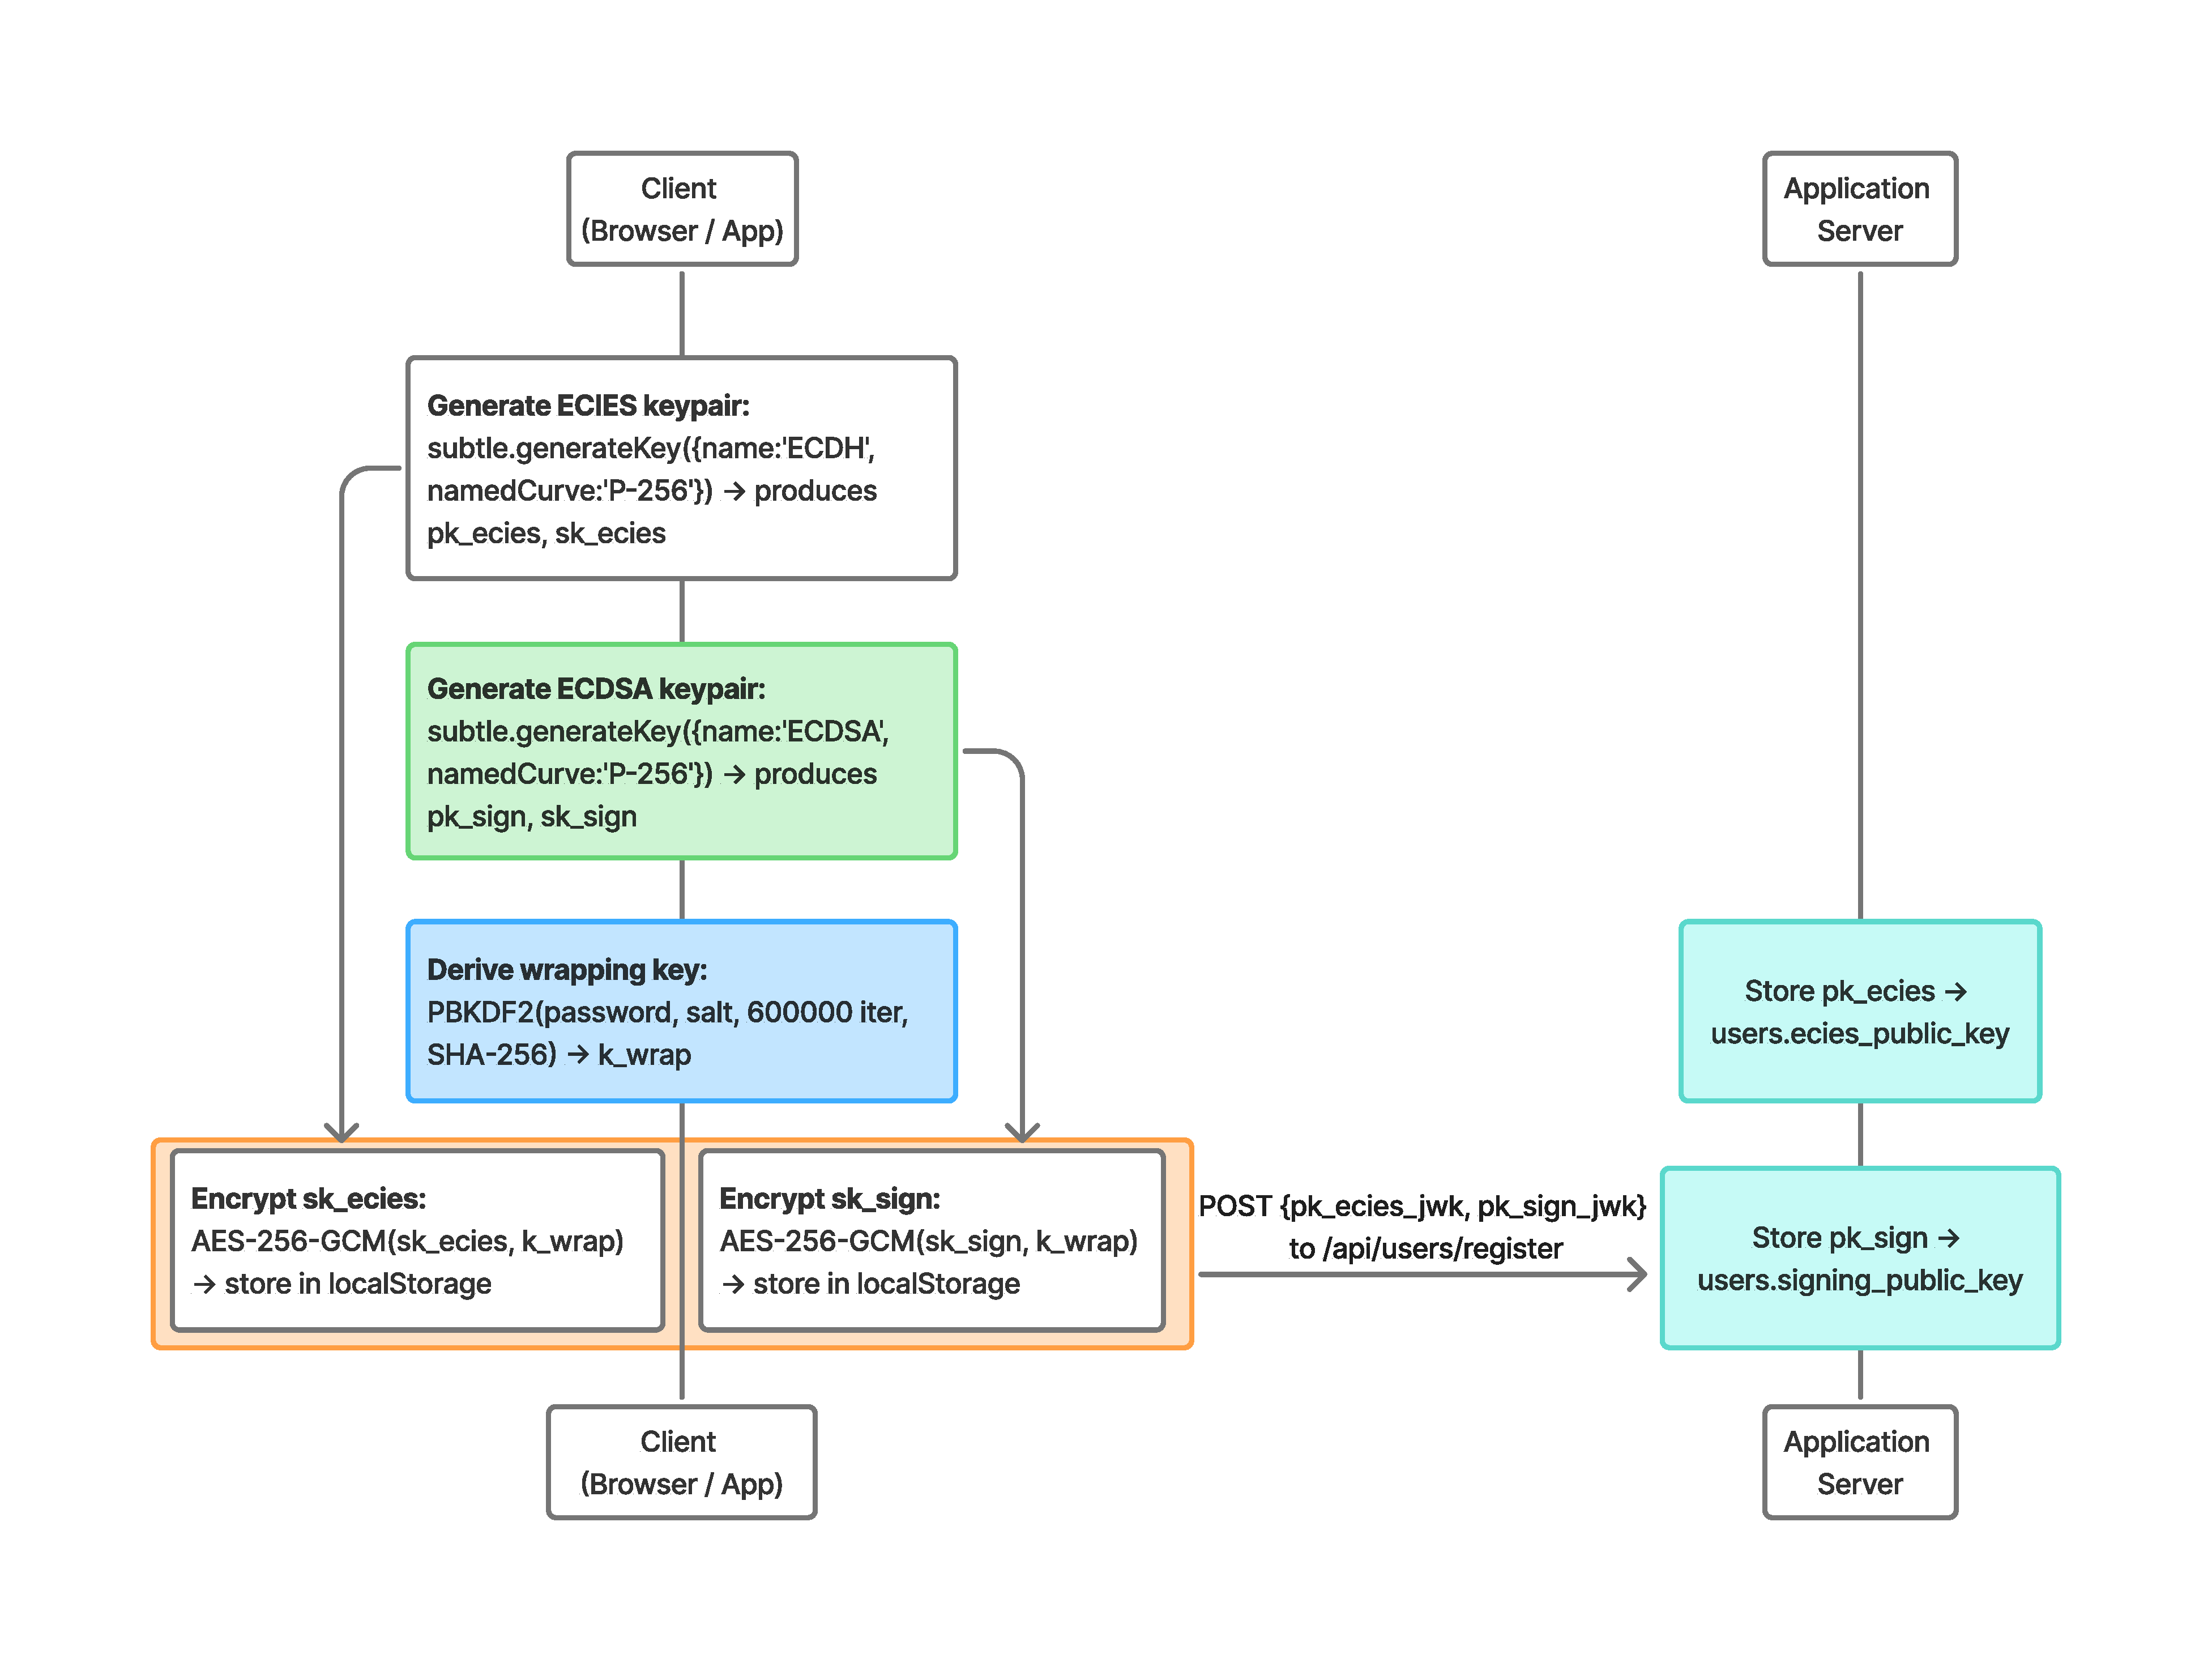
\includegraphics[width=\columnwidth]{key_gen_and_storage.pdf}
    \caption{Phase~1: Client-side key generation. ECIES/ECDSA keys wrapped via PBKDF2-derived key and stored in \texttt{localStorage}, per NIST SP~800-131A key-separation practice.}
    \label{fig:key_gen_and_storage}
\end{figure}

\begin{figure}[!t]
    \centering
    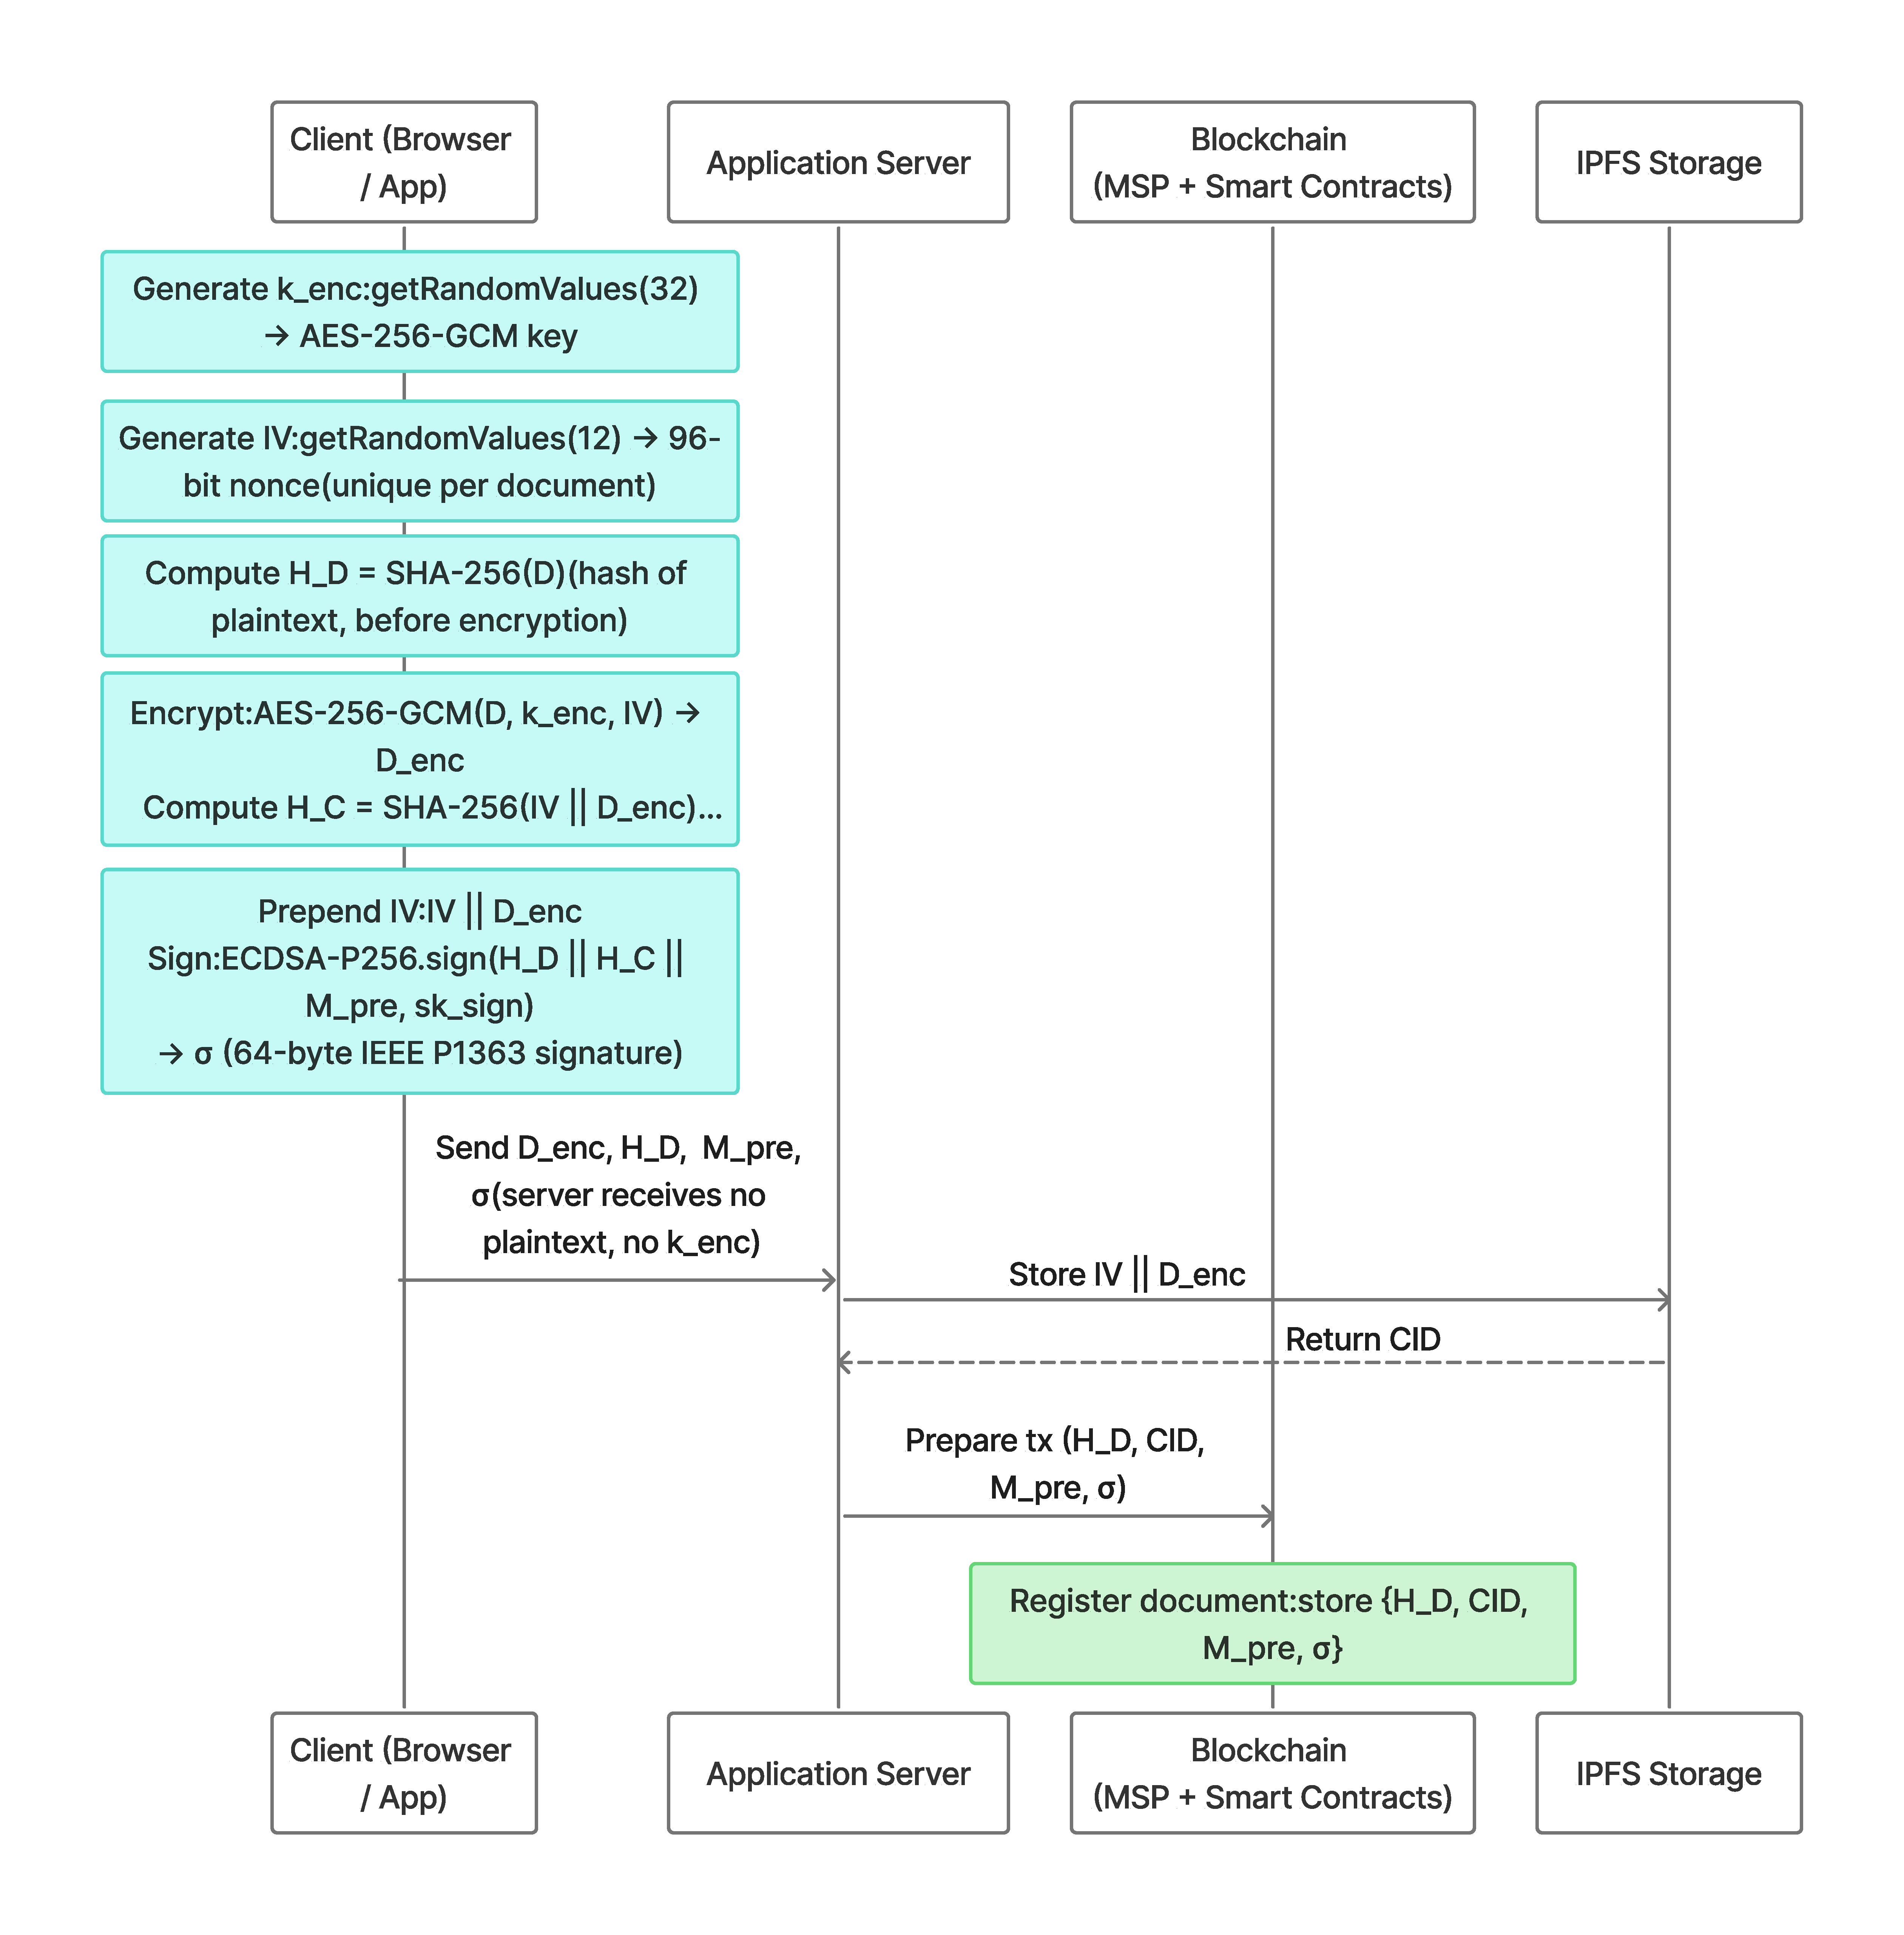
\includegraphics[width=\columnwidth]{document_encryption.pdf}
    \caption{Phase~2 browser-side document encryption and registration with plaintext hashing before encryption, IV-prepended ciphertext, and ECDSA sign-then-store ordering.}
    \label{fig:document_encryption_registration}
\end{figure}

\begin{figure}[!t]
    \centering
    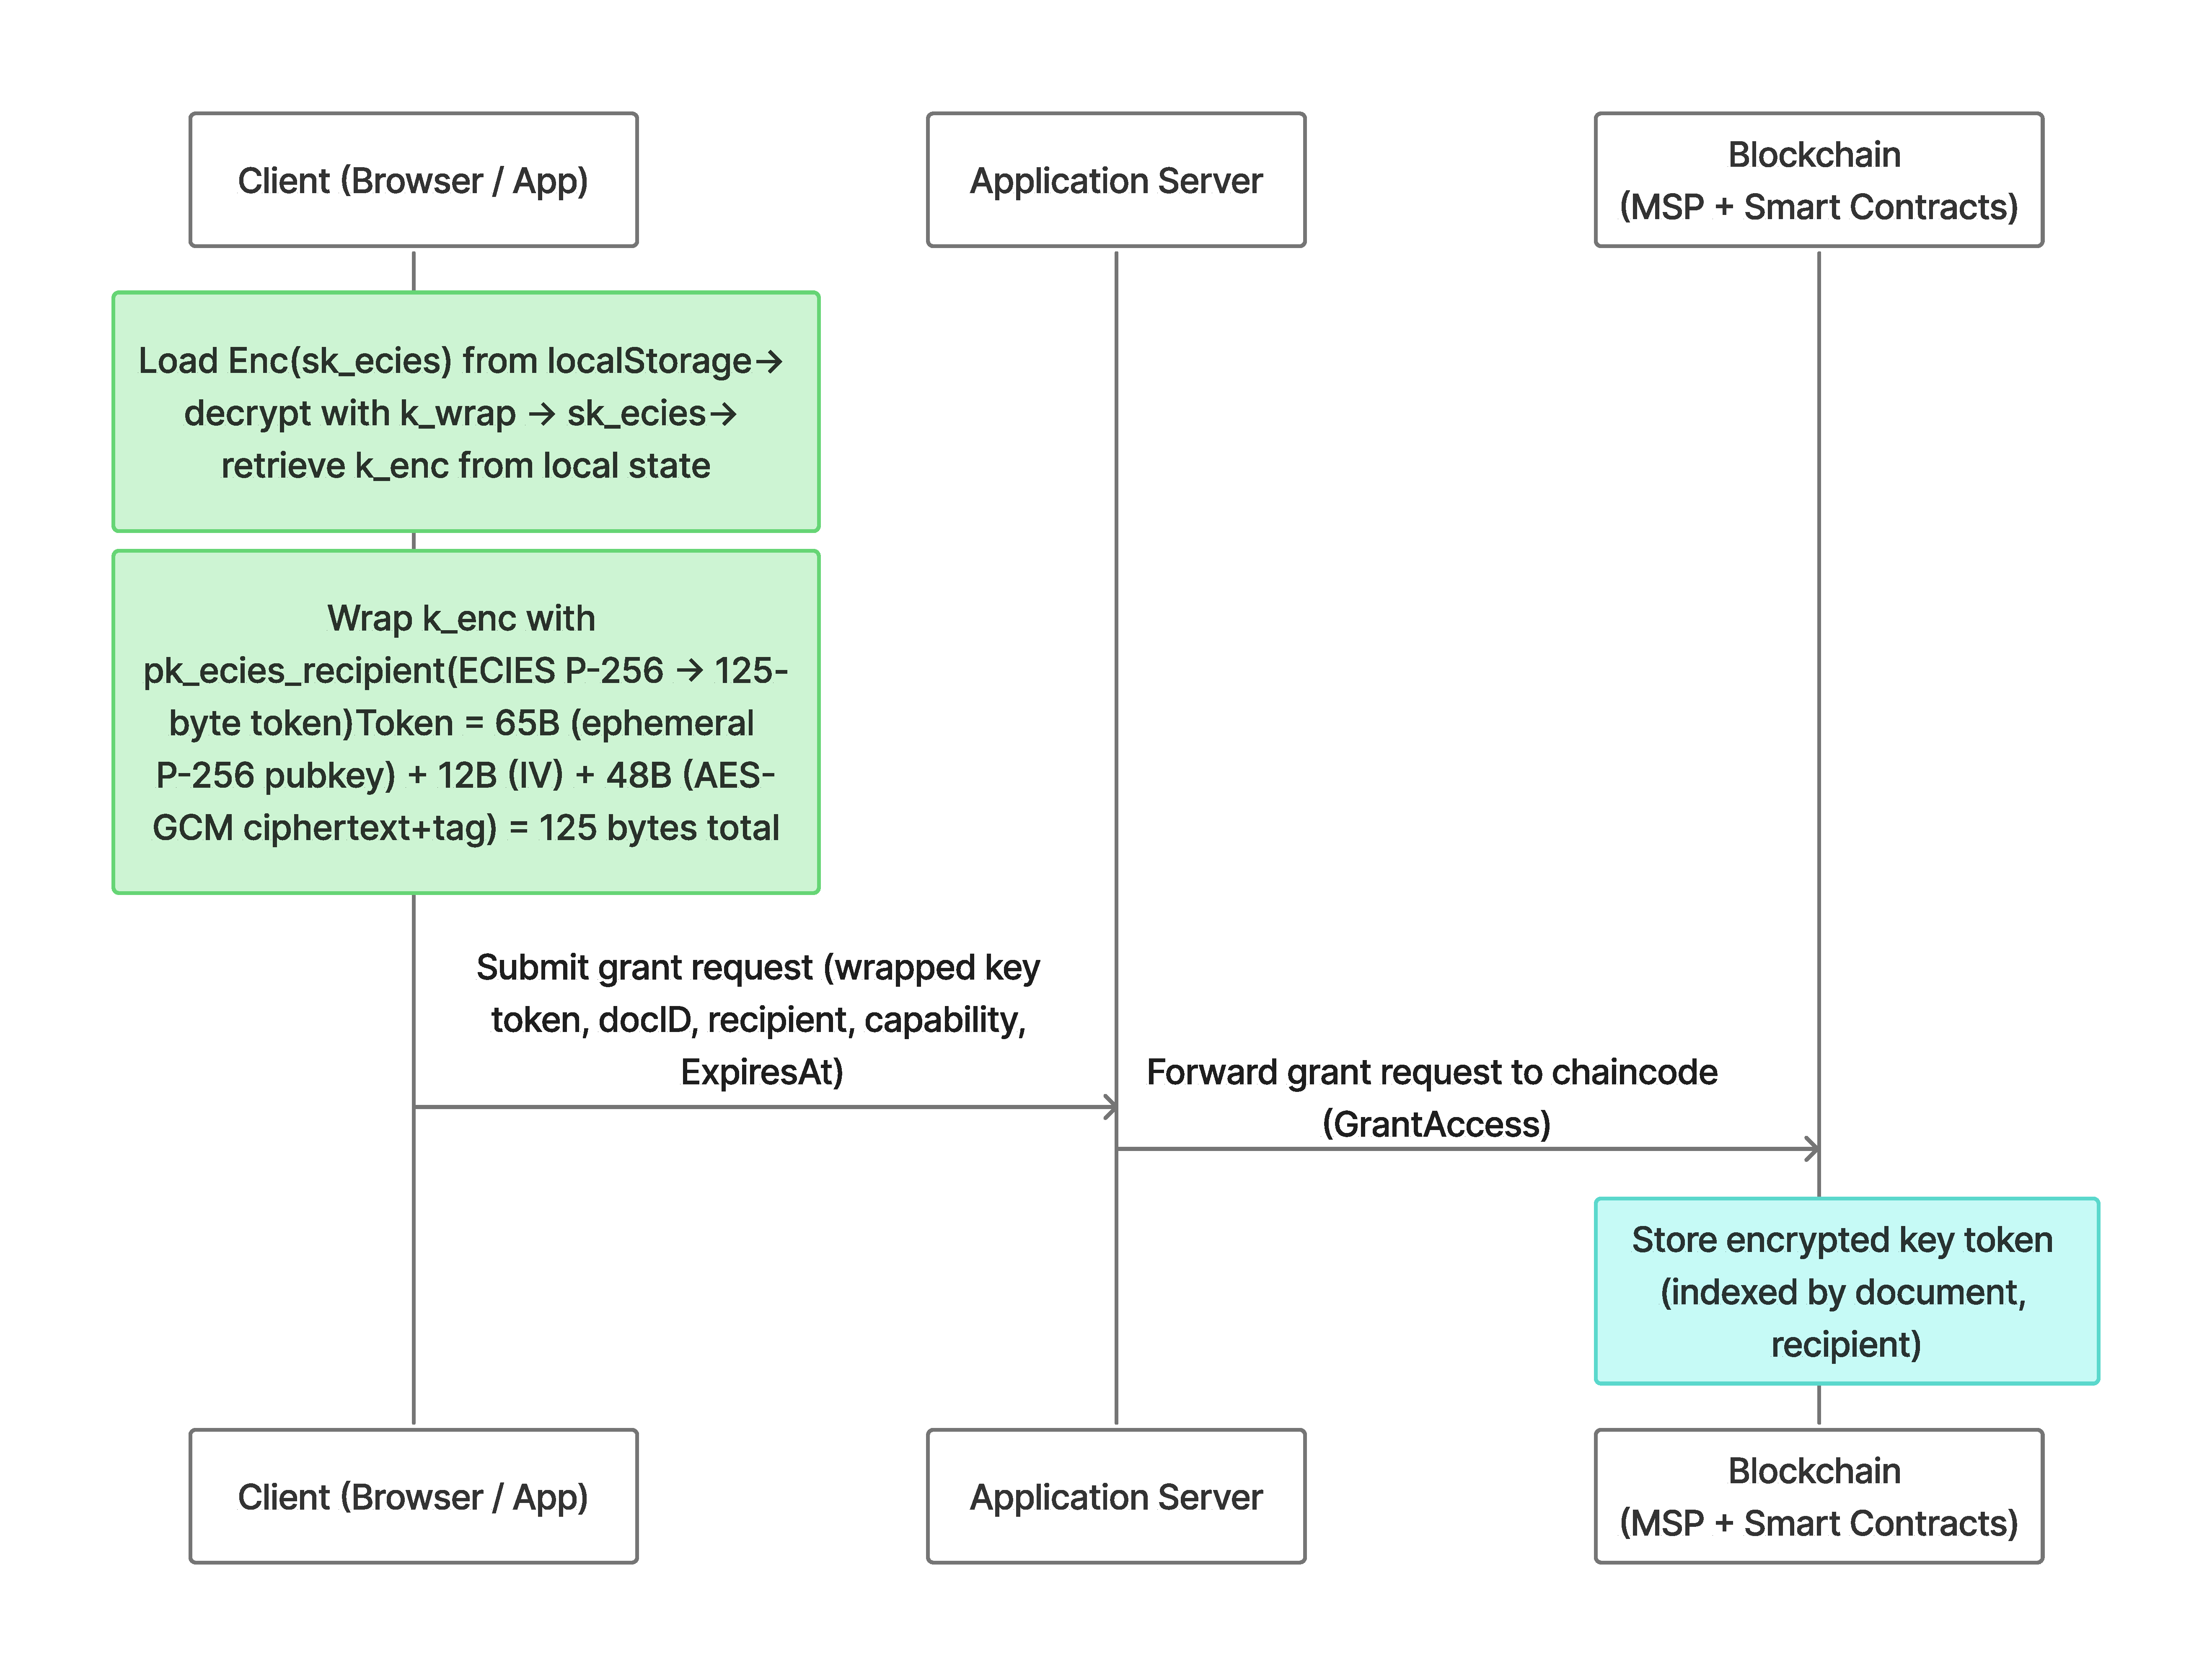
\includegraphics[width=\columnwidth]{access_grant.pdf}
    \caption{Phase~3 ECIES-style P-256 key wrapping, showing owner-wrapped $k_{enc}$, on-chain \texttt{GrantAccess} storage, and ECIES/RSA-OAEP token-size comparison.}
    \label{fig:access_grant_key_distribution}
\end{figure}

\begin{figure}[!t]
    \centering
    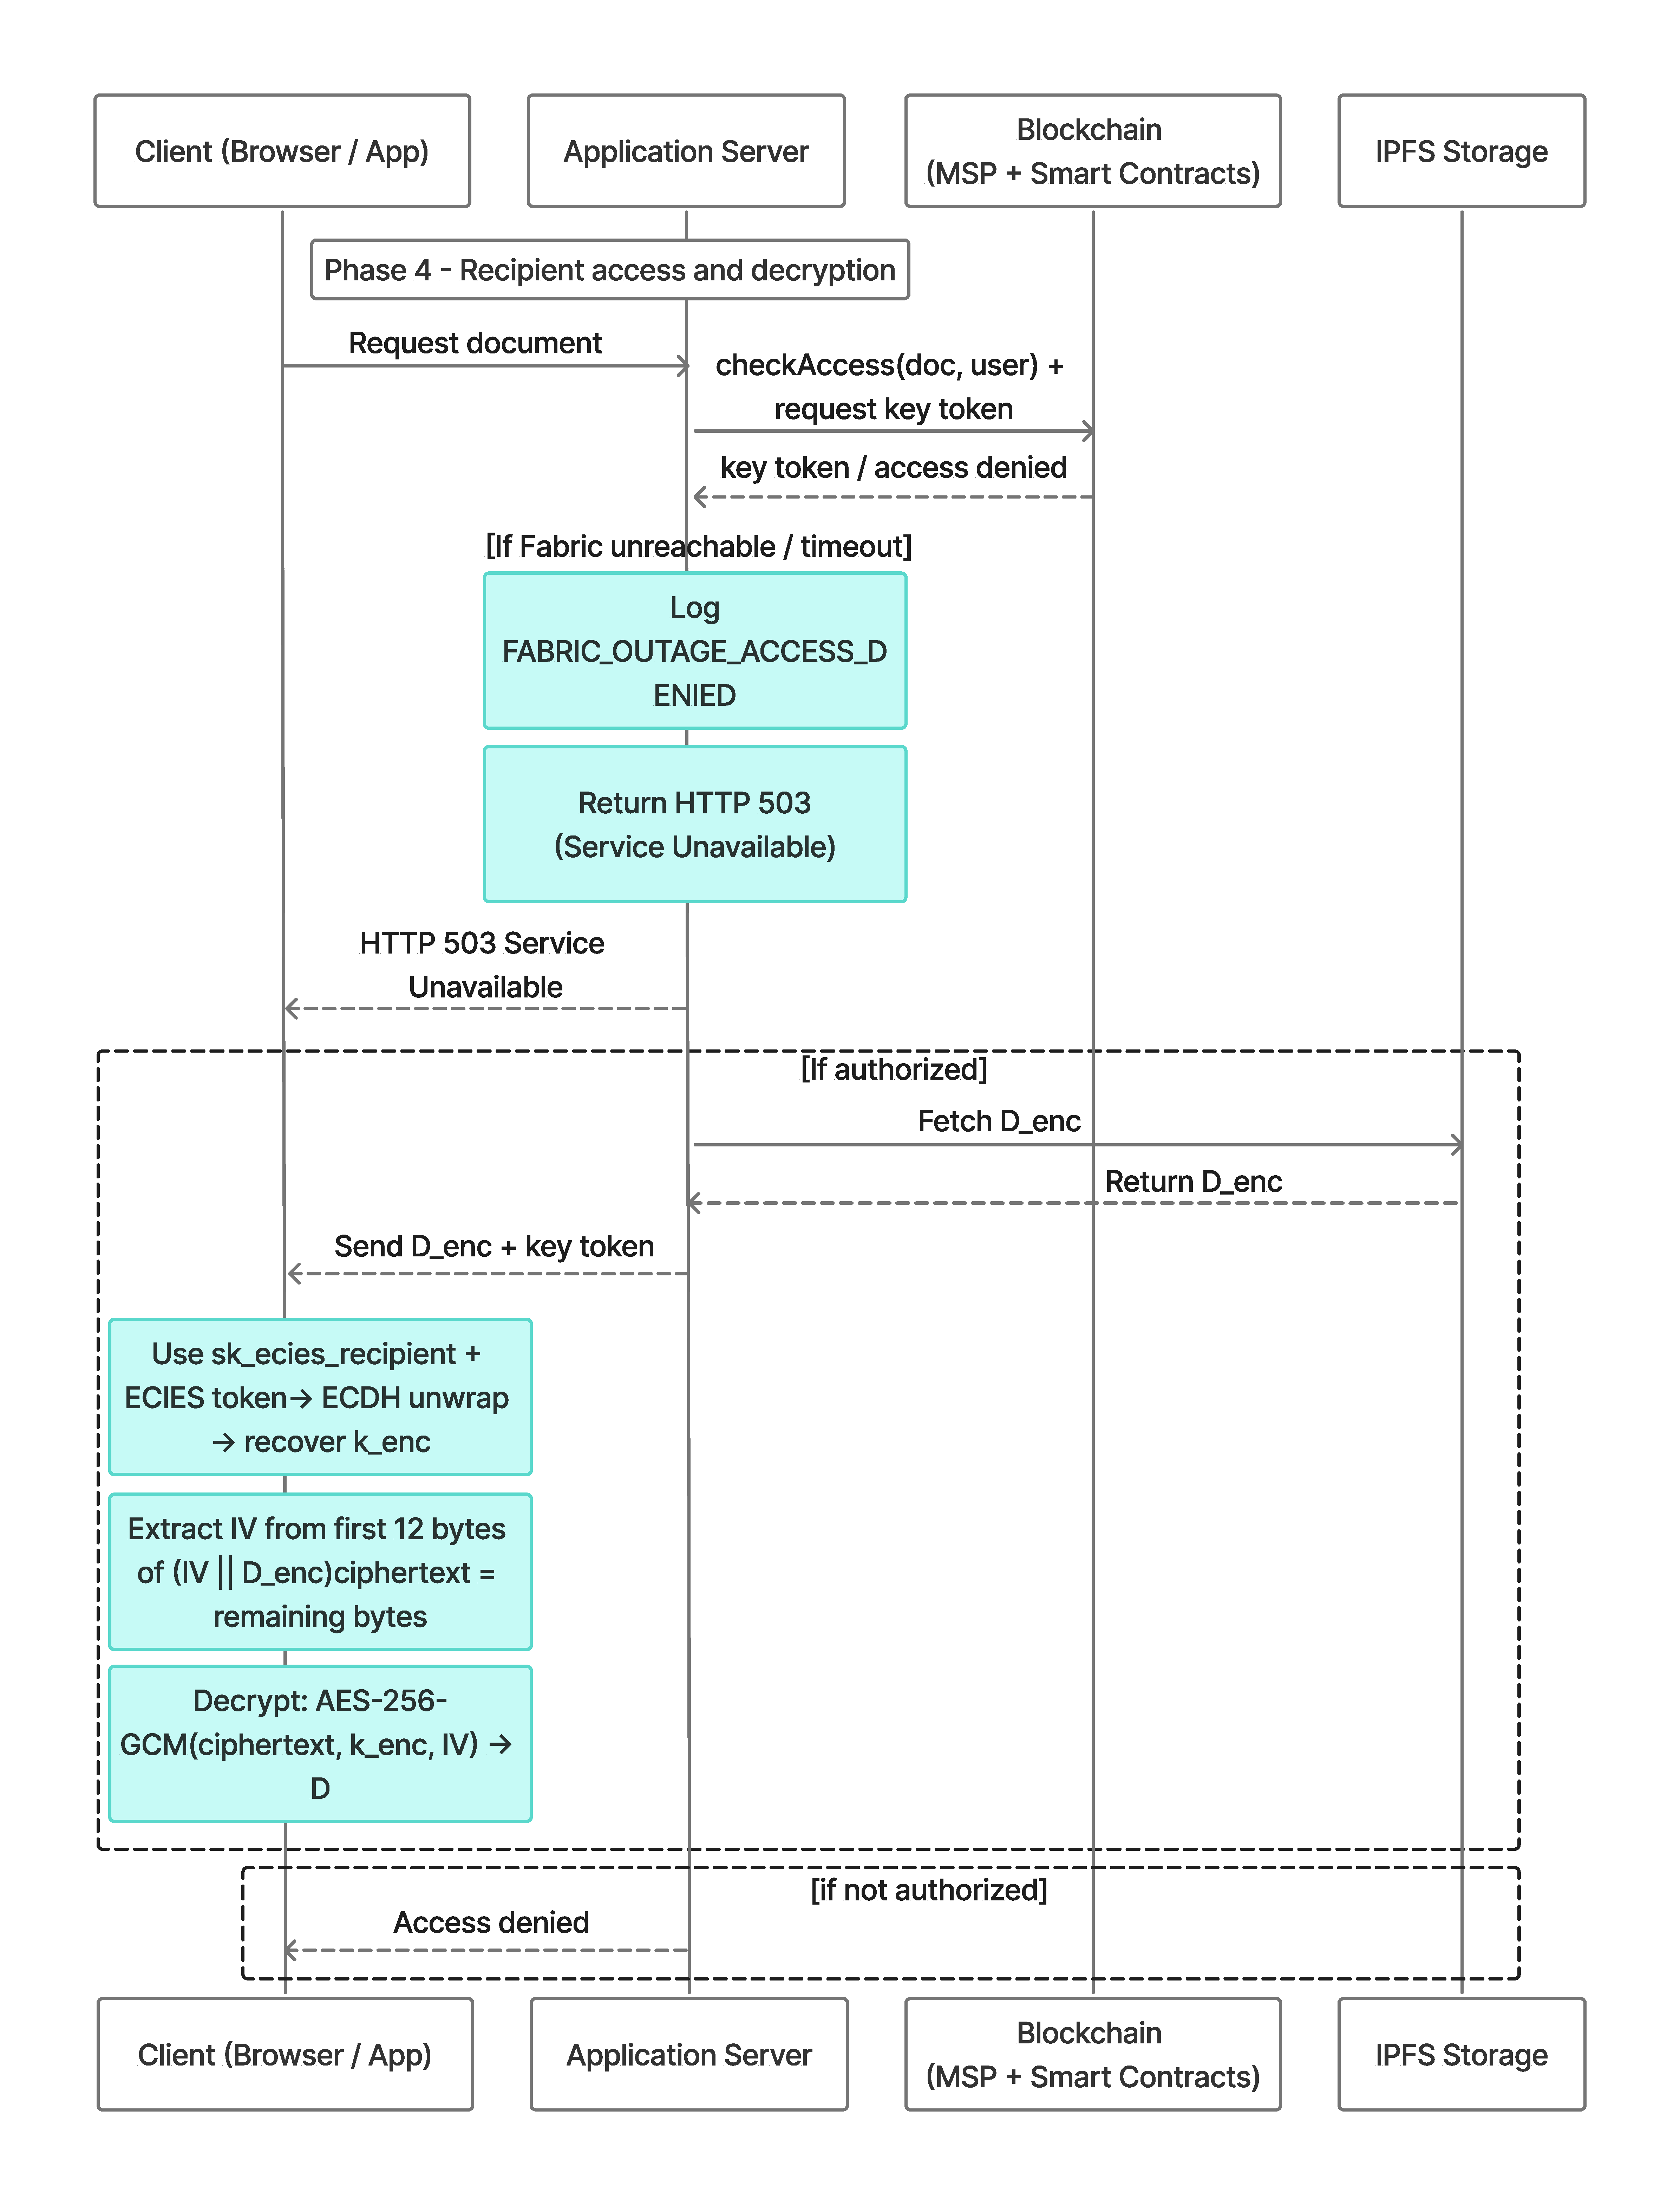
\includegraphics[width=0.95\columnwidth]{access_and_decryption.pdf}
    \caption{Phase~4: Recipient unwraps $k_{enc}$ with $sk_{ecies}$,
    extracts IV from first 12~bytes of stored ciphertext, and decrypts
    locally. Server delivers only ciphertext and wrapped key token.}
    \label{fig:access_and_decryption}
\end{figure}

\begin{figure}[!t]
    \centering
    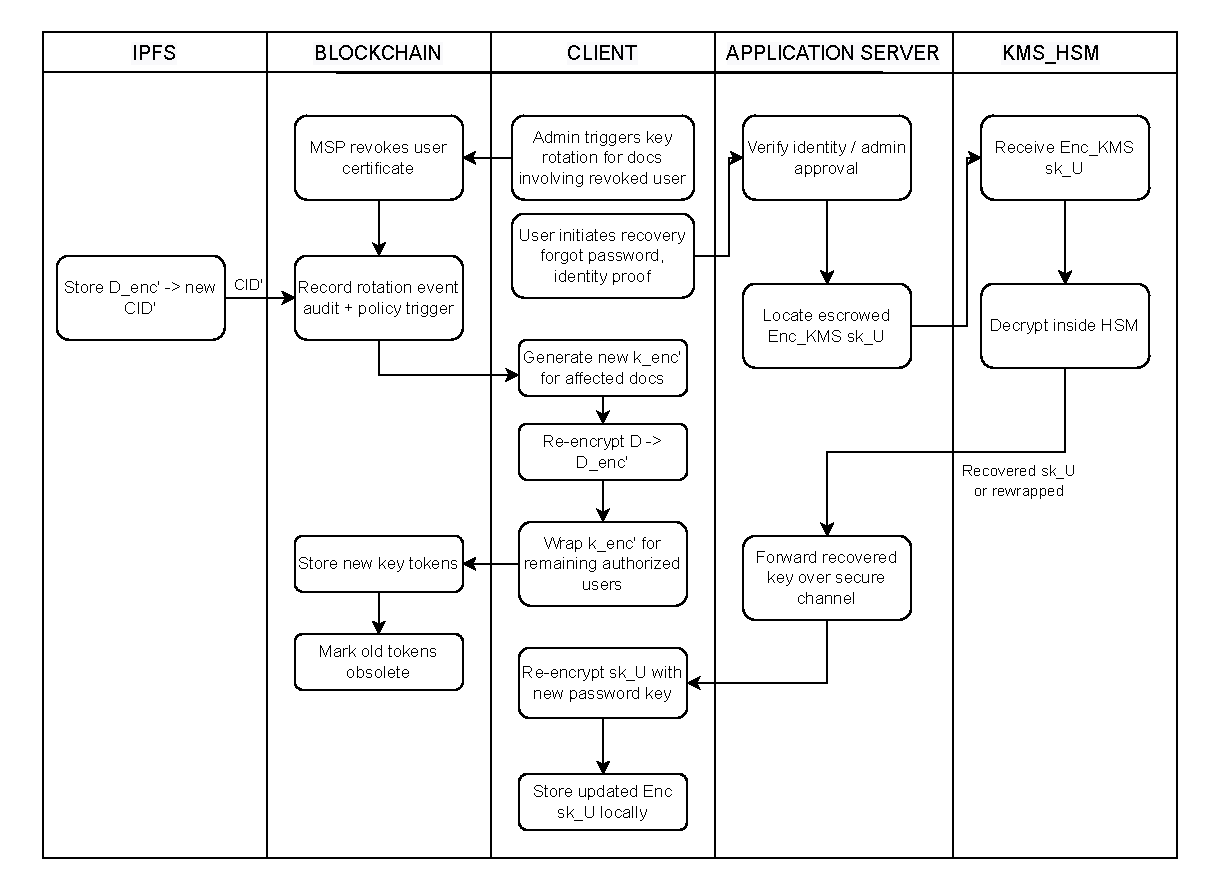
\includegraphics[width=\columnwidth]{key_rotation_and_recovery.pdf}
    \caption{Phase~5: Key recovery via consortium KMS/HSM and
    revocation workflow (framework design, not implemented in prototype).
    Re-encryption requires the document owner's browser; the server does
    not hold $k_{enc}$.}
    \label{fig:key_rotation_and_recovery}
\end{figure}

\subsection{Two-Layer Access Control Architecture}
\label{sec:acl}

Access control is enforced in two independent layers, both of which
must grant a request before any ciphertext is served.

\textbf{Layer~1} is enforced by Spring Security at the API gateway
using JWT-validated role permissions~\cite{rfc7519jwt,RBACSandhu}.
The \texttt{@PreAuthorize} annotation on the service method rejects
requests that fail role validation before any business logic
executes.

\textbf{Layer~2} is enforced by the \texttt{CheckAccess} chaincode
invoked within the service method. The chaincode evaluates access
through a single \texttt{ACL} map using two key conventions: per-user
grants are stored under the user identifier (\texttt{ACL[userID]}), and
organization-level grants are stored under a prefixed key
(\texttt{ACL["ORG:"+userOrg]}). Both per-user and organization-level
grants support time-bounded expiry evaluated at query time. The owner
organization retains implicit read access via the \texttt{doc.OwnerOrg ==
userOrg} fallback. To prevent Multi-Version Concurrency Control (MVCC) conflicts and ledger bloat under high concurrent read loads, the chaincode dynamically evaluates expiry but does not attempt a state write-back during the read path. To maintain strict audit fidelity in the CouchDB world state without introducing read-path latency, the system design relies on a dedicated, asynchronous administrative chaincode invocation (\texttt{CleanExpiredTokens}) executed periodically as a background cron-job to formally deprecate expired tokens.  Listing~\ref{lst:checkaccess} shows the chaincode implementation. Token deprecation therefore follows an \emph{eventual consistency} model: expiry is enforced immediately at chaincode evaluation time, but the CouchDB world state reflects \texttt{StatusExpired} only after the next \texttt{CleanExpiredTokens} invocation; a direct world-state query between these two points will show the token as \texttt{StatusActive} despite being denied at runtime.

% Listing 4 - Go CheckAccess chaincode
\begin{lstlisting}[language=Go,
    caption={\texttt{CheckAccess} chaincode enforcing time-bounded
capability tokens (see Section~\ref{sec:acl} for the eventual-consistency
model). All five access branches shown: per-user grants (Branches~1--2),
owner-organization fallback (Branch~3), and org-prefix grants
(Branches~4--5).},
    label=lst:checkaccess]
// chaincode/legalcc/chaincode.go
func (c *LegalContract) CheckAccess(
    ctx contractapi.TransactionContextInterface,
    docID, userID, userOrg string,
) (string, error) {
  doc, err := getDocument(ctx, docID)
  if err != nil { return "false", err }
  if doc.Status != StatusActive {
    return "false", nil
  }
  txTimestamp, err := ctx.GetStub().
      GetTxTimestamp()
  if err != nil {
    return "", fmt.Errorf(
        "failed to get tx timestamp: %w", err)
  }
  now := time.Unix(txTimestamp.Seconds, 0).UTC()
  if grant, ok := doc.ACL[userID]; ok &&
      grant.Status == StatusActive {
    if grant.ExpiresAt == "" {
      return "true", nil
    }
    exp, err := time.Parse(time.RFC3339,
        grant.ExpiresAt)
    if err == nil && now.Before(exp) {
      return "true", nil
    }
    grant.Status = StatusExpired
    // NOTE: No state write-back occurs here. Expiry is
    // evaluated dynamically on every invocation to avoid
    // MVCC read-write conflicts under concurrent load;
    // StatusExpired is only persisted later by the
    // asynchronous CleanExpiredTokens background job.
    return "false", nil
  }
  if doc.OwnerOrg == userOrg {
    return "true", nil
  }
  // Branch 4-5: org-prefix grant
  if grant, ok := doc.ACL["ORG:"+userOrg]; ok &&
      grant.Status == StatusActive {
    if grant.ExpiresAt == "" {
      return "true", nil
    }
    if exp, err := time.Parse(time.RFC3339,
        grant.ExpiresAt); err == nil &&
        now.Before(exp) {
      return "true", nil
    }
  }
  return "false", nil
}
\end{lstlisting}

On the evaluated document-download path, Fabric unavailability causes
HTTP~503 denial and no database ACL fallback. Other Fabric-gateway paths
follow the same fail-closed pattern by design but were not independently
outage-tested. The service immediately logs a
\texttt{FABRIC\_OUTAGE\_ACCESS\_DENIED} audit event containing the
failure reason and throws a \texttt{ServiceUnavailableException},
returning HTTP~503 to the caller. This prevents new document releases
through this path during the tested Fabric outage and prevents a malicious
actor from using a Fabric disruption to bypass the chaincode authorization
layer. Listing~\ref{lst:download} (Appendix~\ref{app:listings}) shows the two-layer
enforcement in the download path. If the requester has no firm or MSP binding,
the service throws \texttt{AccessDeniedException} before invoking the
Fabric gateway, ensuring the download path is fail-closed
unconditionally for unauthenticated or incomplete principal bindings.

% Listing 5 - Java two-layer ACL download


The complete two-layer enforcement path is summarized in
Fig.~\ref{fig:rbac_acl_pipeline}, and
Algorithm~\ref{alg:access_grant} formalizes the capability-grant
construction.

\begin{figure*}[!t]
    \centering
    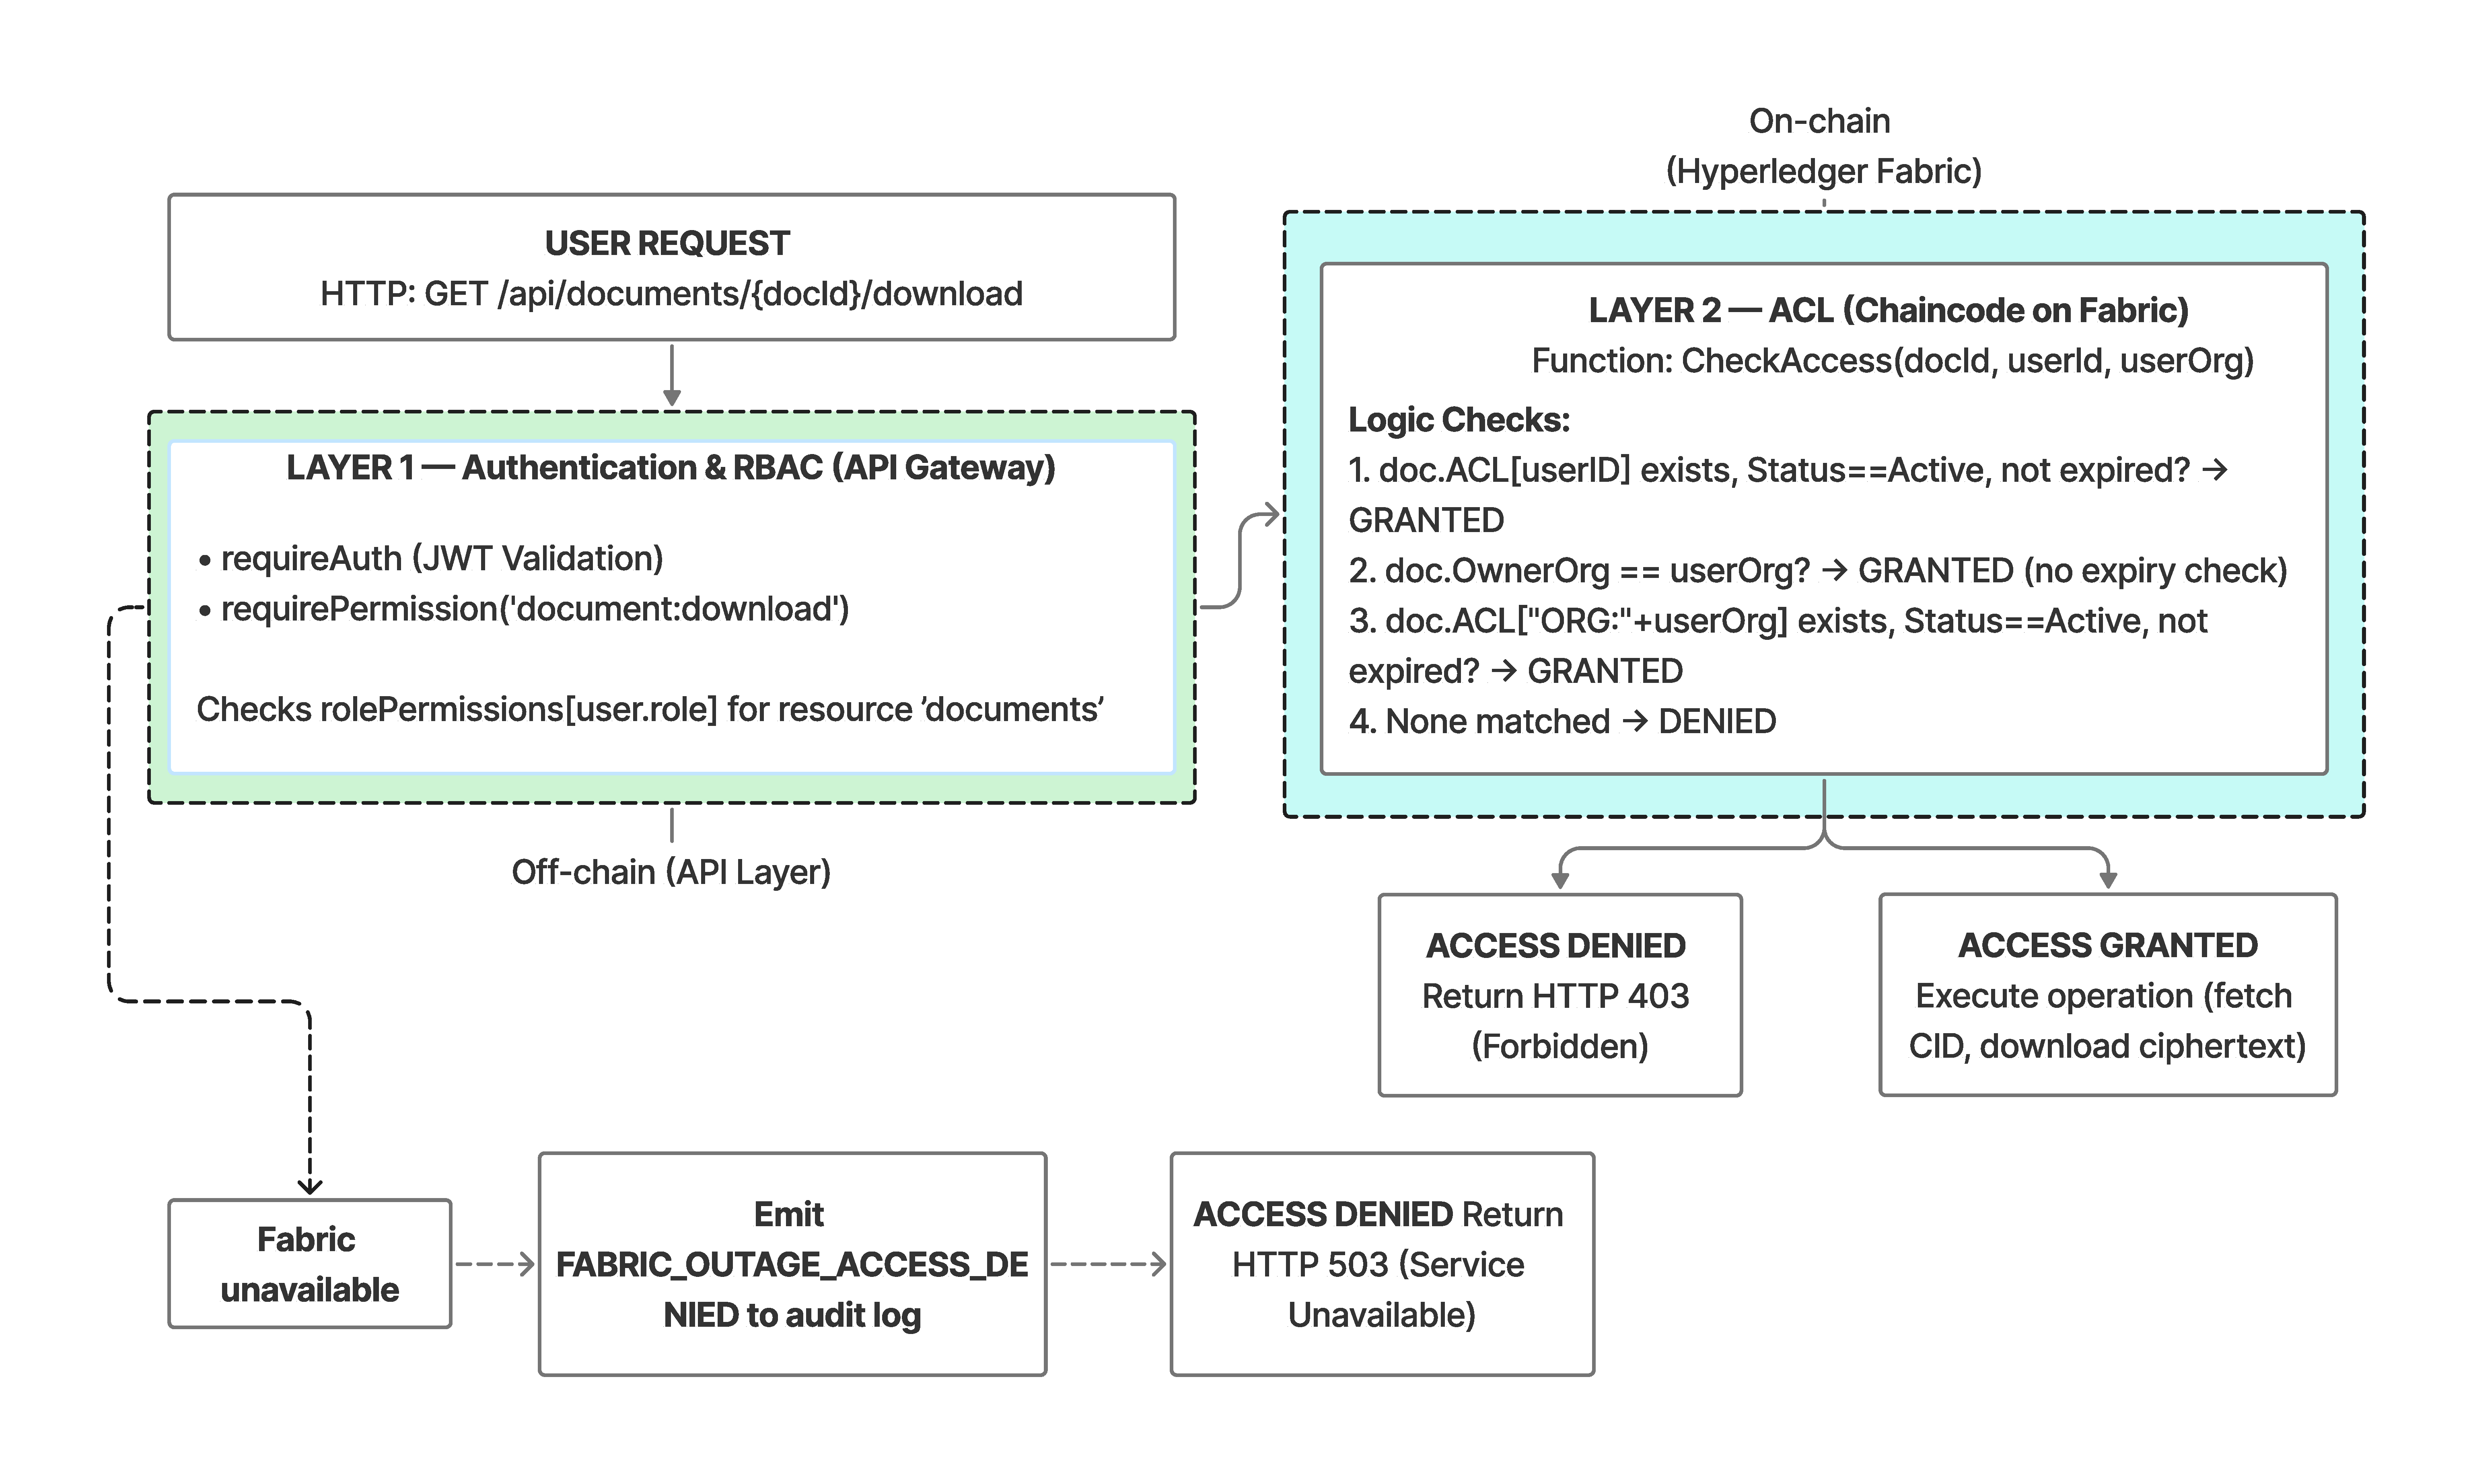
\includegraphics[width=0.82\textwidth]{rbac_acl_pipeline.pdf}
    \caption{Two-layer access control pipeline: API-gateway JWT RBAC, on-chain \texttt{CheckAccess}, and fail-closed \texttt{FABRIC\_OUTAGE\_ACCESS\_DENIED} blocking.}
    \label{fig:rbac_acl_pipeline}
\end{figure*}

\begin{algorithm}[H]
\caption{Capability-Based Access Grant}
\label{alg:access_grant}
\scriptsize
\begin{algorithmic}[1]
\REQUIRE Document ID $d$, subject $s$, permission $p$, conditions $\mathcal{C}$
\ENSURE Capability token $T$ or $\perp$
\STATE $t_{exp} \leftarrow t_{now}+\mathcal{C}.\Delta t$ \COMMENT{$\Delta t=\infty$ if no expiry}
\STATE $S_{scope} \leftarrow \text{Parse}(\mathcal{C}.scope)$
\STATE $T \leftarrow (d,s,p,t_{exp},S_{scope})$
\STATE $\sigma_T \leftarrow \text{ECDSA-P256.Sign}(\mathcal{H}(T),sk_{grantor})$
\STATE $\mathcal{R} \leftarrow \{\mathcal{C}.\text{triggers}\}$
\STATE \textbf{Blockchain.Store}$(\langle T,\sigma_T,\mathcal{R}\rangle)$
\STATE \textbf{emit} \texttt{ACCESS\_GRANTED}$(d,u_{grantor}\rightarrow s)$
\STATE \textbf{return} $T$
\end{algorithmic}
\vspace{-0.4em}
\end{algorithm}

\subsection{Audit Architecture}
\label{sec:audit}

The system maintains two independent audit stores by design. Their
independence is a deliberate security property, but the two stores
provide different guarantees.

\textbf{Fabric ledger (primary, cryptographic).} Every significant
event is recorded by the \texttt{LogAuditEvent} chaincode as an
immutable ledger transaction. Any consortium peer can query the
history of any document key using \texttt{GetHistoryForKey}, which
returns a chronologically ordered, hash-linked sequence of state
transitions. The Fabric block hash chain provides cryptographic
tamper-evidence natively; the application does not maintain a
separate SHA-256 chain over on-chain records because doing so would
be redundant with Fabric's own block structure.

\textbf{PostgreSQL \texttt{audit\_log} (secondary, operational).}
A separate append-only table records all events for fast dashboard
queries. An INSERT-only enforcement trigger at the database level
raises an exception on any UPDATE or DELETE attempt regardless of
application privileges. A TRUNCATE-prevention trigger closes the
PostgreSQL DDL bypass gap, and TRUNCATE privilege is revoked from
all application roles at the schema level.
Listing~\ref{lst:audittrigger} (Appendix~\ref{app:listings}) shows both triggers. These triggers
are an \emph{operational convenience} that raises the bar against
accidental or application-layer modification; they are not a
security defense against a database administrator with superuser
access. A superuser can drop triggers, alter the schema, or bypass
the SQL engine entirely via direct file access, rendering the
trigger layer ineffective against the Malicious DB Administrator
adversary class defined in Table~\ref{tab:threat_model}. The
security guarantee against that adversary relies entirely on the
Fabric ledger, which the database administrator cannot access or
modify: any consortium peer can independently verify the complete
audit trail via \texttt{GetHistoryForKey} without trusting the
application server or its database~\cite{androulaki2018hyperledger}.

% Listing 6 - SQL audit triggers


Experiment~\hyperref[sec:exp_audit]{4} (Section~\ref{sec:exp_audit}) measures PostgreSQL
\texttt{audit\_log} query P50 at 3.9\,ms for 1,000 events on Linux
\texttt{x86\_64}, and Experiment~\hyperref[sec:exp_gethistory]{7}
(Section~\ref{sec:exp_gethistory}) measures Fabric
\texttt{GetHistoryForKey} at 135.5\,ms P50 for a 107-entry document
history. The two stores serve complementary roles: PostgreSQL supports
low-latency operational dashboards, while Fabric provides
cryptographic non-repudiation and independent verification by any
consortium peer without trusting the application server.

% =========================================================================
% SECTION IV --- GOVERNANCE, SECURITY, CONSENSUS
% =========================================================================
\section{Governance, Security, and Consensus}
\label{sec:governance_security}

\subsection{Operational Threat Model}
\label{sec:threat_model}

This section defines the operational security assumptions under which
the framework is evaluated. The goal is not to present a new
cryptographic proof, but to make explicit which adversaries are in
scope, which trust boundaries are enforced by Fabric, and which risks
remain in the measured prototype. The analysis covers consortium
governance assumptions, Raft crash-fault-tolerant ordering limits,
endorsement-policy limits, application and browser compromise,
identity-management boundaries, on-chain metadata leakage, and
residual risks requiring production hardening.

The deployment model is a permissioned legal consortium consisting of
known, legally bound institutions such as law firms and a regulator.
Participants are authenticated through Fabric MSPs, and state-changing
transactions are validated by endorsement policies before being
ordered and committed. Under normal operation, document access is
evaluated through the \texttt{CheckAccess} chaincode before protected
material is released. On the evaluated document-download path, Fabric
unavailability causes HTTP~503 denial and no database ACL fallback. Other
Fabric-gateway paths follow the same fail-closed pattern by design but
were not independently outage-tested. The threat
model therefore identifies the custodial Fabric identity and
\texttt{localStorage}-based key handling as the primary residual
prototype limitations, not a database fallback.

\textbf{Bounded adversary assumption.} Two independent bounds apply:
(1)~\emph{CFT orderer bound}: with a 3-node Raft cluster ($n=3$),
the crash-fault tolerance bound is $f \leq \lfloor(n-1)/2\rfloor =
1$; the cluster tolerates failure of any single ordering node while
maintaining consensus progress~\cite{Ongaro2014}. This bound applies
to node crashes, not Byzantine behavior. (2)~\emph{Endorsement
policy bound}: when a deployment requires
\texttt{AND(}\allowbreak\texttt{'LawFirmAMSP.peer',}\allowbreak
\texttt{'RegulatorMSP.peer')}, an adversary
cannot satisfy that policy by controlling a single organization,
because both organizations' peer endorsement is required
independently. These bounds are independent: orderer
quorum governs block formation; endorsement policy governs state
write validity. The adversary may be adaptive but cannot break the
cryptographic primitives (AES-256-GCM, ECDSA~P-256, SHA-256) under
their standard hardness assumptions.

The prototype's ECIES grants are ledger-recorded but depend on an
off-chain identity-to-key binding: PostgreSQL stores each user's
\texttt{pk\_ecies} and \texttt{pk\_sign}. Until these public keys are
anchored by a \texttt{RegisterIdentity}-style ledger transaction, a
database or API adversary who substitutes \texttt{pk\_ecies} before a
grant is formed can cause future \texttt{GrantAccess} operations to
wrap $k_{enc}$ to an attacker-controlled key. Fabric would then commit
a cryptographically valid transaction whose recipient key binding is
semantically wrong. This threat is distinct from direct ledger
tampering and is treated as a highest-priority production hardening
requirement.

Table~\ref{tab:threat_model} identifies seven adversary classes
relevant to the legal consortium deployment.



\begingroup
\scriptsize
\renewcommand{\arraystretch}{1.15}
\begin{xltabular}{\textwidth}{|p{2.2cm}|X|p{2.0cm}|X|X|}
\caption{Operational Threat Model: Adversary Classes and System
Defenses. This is a structured adversary analysis, not a formal
cryptographic security proof. Residual risk column identifies
properties that require governance controls or hardware beyond
the current prototype.}
\label{tab:threat_model}\\
\hline
\textbf{Adversary} & \textbf{Capabilities} &
\textbf{Property threatened} &
\textbf{System defense} & \textbf{Residual risk} \\
\hline
\endfirsthead
\multicolumn{5}{l}{\textit{Table \thetable\ (continued)}}\\
\hline
\textbf{Adversary} & \textbf{Capabilities} &
\textbf{Property threatened} &
\textbf{System defense} & \textbf{Residual risk} \\
\hline
\endhead
\hline
\endfoot
\endlastfoot
Honest-but-curious peer &
Can observe all transactions on joined channels; can read world state;
cannot modify ledger or forge signatures &
Confidentiality of document content and access patterns &
Documents stored as AES-256-GCM ciphertext in private IPFS swarm;
CIDs and hashes only on-chain; PDCs limit metadata to authorized
peers~\cite{fabricPDCDoc} &
Channel members still see CIDs, timestamps, accessor MSP identities,
PDC hashes, and plaintext hash \(\mathcal{H}_D\), leaking frequency
patterns and enabling candidate-document confirmation via local
\texttt{SHA-256}. The prototype uses organization-level membership
(\texttt{doc.OwnerOrg == userOrg}) as first-pass control; per-user
intra-organization ACLs and moving \(\mathcal{H}_D\) to a PDC or keyed
commitment \(\text{HMAC}_k(D)\) remain production hardening. \\
\hline
Malicious DB administrator &
Full write access to PostgreSQL; can modify application tables;
cannot access Fabric peers or IPFS directly &
Integrity of access control records and audit log &
Under normal operation, access control is evaluated by chaincode
(Layer~2). During Fabric unavailability, the system fails closed 
(returning HTTP 503). The \texttt{audit\_log} row-level
and statement-level triggers block accidental or application-layer
modification and TRUNCATE attempts (Listing~\ref{lst:audittrigger}) &
Triggers provide operational integrity only, not cryptographic
protection from a PostgreSQL superuser. The DB admin cannot directly
alter Fabric ACL or audit history, and Fabric outages deny access;
however, replacing \texttt{pk\_ecies} can make later grants wrap
$k_{enc}$ to an attacker key while the ledger records an apparently
valid grant. Null firm/MSP now raises \texttt{AccessDeniedException}
before the Fabric gateway; no default organization is assumed
(Listing~\ref{lst:download}). \\
\hline
Compromised application server / API operator &
Controls the Spring Boot service, API-layer RBAC middleware, REST gateway, and operational database access; may attempt to bypass chaincode, misuse
server-managed Fabric MSP credentials, serve tampered frontend
JavaScript to intercept client-side operations, cache or forward IPFS
ciphertext after legitimate delivery, or abuse MSP identity bindings
before ledger commitment &
Authorization integrity, transaction attribution, confidentiality in
prototype plaintext-handling paths &
In the honest-code normal path, document release invokes
\texttt{CheckAccess} against ledger-visible ACL state before protected
material is returned. Fabric provides an independently verifiable
record for ledger-mediated grants, revocations, and audit events; Fabric outage events log as \texttt{FABRIC\_OUTAGE\_ACCESS\_DENIED}; user-level
document signatures bind the signing key to $\mathcal{H}_D$, $\mathcal{H}_C$, and $id_D$ &
A fully compromised API operator can bypass application logic, misuse
custodial MSP credentials, expose plaintext via malicious frontend
delivery before browser encryption, abuse off-chain access paths, or
substitute recipient keys before grant creation. Fabric still makes
ledger-mediated state changes auditable; production requires
browser-only encryption, per-user Fabric identities, ledger-anchored
public keys, and strict service hardening. \\
\hline
Compromised browser / XSS attacker &
Executes malicious JavaScript in the user's browser session; can
observe passwords or decrypted private keys during unlock/use; can
initiate actions as the logged-in user; may tamper with frontend code
before encryption or signing &
Client-side key confidentiality, document confidentiality before
encryption, and authenticity of user-initiated actions &
Private keys are stored encrypted in browser \texttt{localStorage}
under a PBKDF2-derived AES-GCM wrapping key; plaintext and signing
operations are intended to occur in the browser; server-side audit
records and Fabric logs make submitted actions traceable &
Encrypted \texttt{localStorage} resists passive storage theft, not
active browser compromise. XSS or malicious frontend code can capture
passwords, plaintext, or keys during use; production requires CSP,
supply-chain controls, WebAuthn/FIDO2 or HSM-backed keys, and hardened
frontend delivery. \\
\hline
Compromised IPFS node &
Can serve modified or stale ciphertext; cannot forge SHA-256 hashes &
Document integrity and availability &
SHA-256 hash of plaintext stored on-chain at registration; any
tampered ciphertext produces a hash mismatch detectable by any
authorized client on download; the design uses a private two-node
swarm/cross-pinning configuration &
Availability still depends on pinning policy and node health. If both
IPFS nodes are compromised or unavailable, content may be unavailable;
production requires $\geq$3 pinning nodes or an SLA-backed pinning
service. \\
\hline
Orderer collusion (1-of-3 Raft) &
A single compromised orderer can observe all unordered transactions;
cannot unilaterally reorder or censor if the 2-of-3 quorum continues
to function &
Transaction ordering integrity and liveness &
3-node Raft: any single orderer failure is tolerated while consensus
continues; Fabric's execute-order-validate pipeline means peers
independently validate every block regardless of orderer
behavior~\cite{androulaki2018hyperledger,
hyperledgerFabricOrderingService_v24} &
Two colluding orderers (2-of-3) can censor or delay transactions; CFT
does not prevent Byzantine ordering. Fabric~v3.0
SmartBFT~\cite{fabricWhatsNew3x,fabricOrderingServiceLatest} is the
production path for high-threat deployments. \\
\hline
On-chain metadata leakage &
Channel members can observe transaction timestamps, invoking MSP
identity, and CIDs even for PDC-protected data &
Access pattern privacy &
PDCs store sensitive metadata in a private collection; only the
collection hash is written to the main ledger~\cite{fabricPDCDoc}.
A channel member observing transaction frequency and CID patterns
over time can infer which documents are accessed frequently,
potentially revealing case activity patterns without decrypting
content &
Traffic analysis can reveal access patterns without document content.
Zero-knowledge proofs, batching, cover traffic, or private access
protocols are future work to reduce leakage
(Section~\ref{sec:future_work}). \\
\hline
\end{xltabular}
\par\vspace{3pt}
\begin{minipage}{\textwidth}
\raggedright\scriptsize
\smallskip
\noindent\textit{Malicious Fabric peer clarification.}
Table~\ref{tab:threat_model} separates honest-but-curious peer observation
from active peer compromise. A malicious Fabric peer may run altered local
software, leak channel or world-state metadata, withhold endorsements, return
misleading query responses, or collude with other organizations. It cannot by
itself commit invalid ledger state when a transaction requires
multi-organization endorsement, because committing peers validate endorsement
signatures, read-write sets, MVCC versions, and chaincode-definition
consistency before updating world state~\cite{androulaki2018hyperledger,
hyperledgerFabricOrderingService_v24}. Residual risks remain if enough
endorsing organizations collude, if clients trust a single peer for query
results, or if channel metadata itself is sensitive; production deployments
therefore require multi-organization endorsement policies, peer monitoring,
query-provenance checks where appropriate, and governance sanctions.
\end{minipage}
\endgroup

\begin{table}[!t]
\centering
\caption{Compact security argument sketch. Residual risks are not eliminated by the prototype.}
\label{tab:security_claims}
\renewcommand{\arraystretch}{1.08}
\setlength{\tabcolsep}{1.8pt}
\tiny
\begin{tabularx}{\columnwidth}{|>{\RaggedRight\arraybackslash}p{1.25cm}|>{\RaggedRight\arraybackslash}p{2.55cm}|>{\RaggedRight\arraybackslash}X|}
\hline
\textbf{Claim} & \textbf{Argument} & \textbf{Residual risk} \\
\hline
Fabric audit history cannot be silently altered by a DB admin &
Fabric is append-only across endorsing peers; PostgreSQL triggers are only operational support~\cite{androulaki2018hyperledger}. &
DB superuser can alter off-chain identity data; production path anchors public keys on-chain. \\
\hline
IPFS ciphertext cannot be modified undetectably &
Plaintext hash $\mathcal{H}_D$ is anchored on-chain; altered ciphertext causes client-side verification failure~\cite{benet2014ipfs}. &
Content availability still needs $\geq$3 pinning nodes or an SLA-backed pinning service. \\
\hline
Fabric outage fails closed &
\texttt{CheckAccess} is on the document-release path; Fabric failure returns HTTP~503 and logs \texttt{FABRIC\_\allowbreak OUTAGE\_\allowbreak ACCESS\_\allowbreak DENIED}. &
None observed on download path; upload, grant, and revoke paths are fail-closed by design but not independently validated. \\
\hline
API compromise remains residual &
ECDSA binds document commitments to user keys, and Fabric records ledger-mediated events; prototype MSP credentials remain server-managed. &
Compromised server can abuse custodial MSP credentials; production requires per-user Fabric identities. \\
\hline
Browser/XSS compromise remains residual &
Keys are PBKDF2-protected in \texttt{localStorage}; signing/decryption are intended to occur client-side. &
Active XSS can capture keys or plaintext; mitigation requires WebAuthn/FIDO2, CSP, and supply-chain controls. \\
\hline
2-of-3 Raft orderer collusion remains residual &
Peers validate blocks independently after ordering~\cite{androulaki2018hyperledger}; governance reduces but does not cryptographically prevent collusion. &
CFT does not stop Byzantine ordering; SmartBFT is the documented high-threat production path~\cite{fabricWhatsNew3x,fabricBFTConfigurationDoc}. \\
\hline
\end{tabularx}
\end{table}

Table~\ref{tab:security_claims} summarizes the principal security claims, their architectural support, and the residual risks left by the current prototype.

The framework uses Raft, a Crash Fault
Tolerant (CFT) protocol. CFT tolerates node failures but not
Byzantine orderer behavior. This choice is a \emph{performance
trade-off}, not a cryptographic security guarantee. Legal
accountability reduces the probability of collusion among orderers
operated by distinct, legally-bound institutions, but provides no
cryptographic bound against Byzantine behavior: a sufficiently
motivated or compromised orderer set can still violate CFT's safety
assumptions. As noted in the threat model table, 2-of-3 orderer
collusion remains a residual risk under CFT, and the current Raft
configuration is a \emph{prototype constraint} rather than a
framework recommendation. For deployments in which Byzantine fault
tolerance is required, the SmartBFT ordering service introduced in
Hyperledger Fabric~v3.0 is the recommended
path~\cite{fabricWhatsNew3x,fabricOrderingServiceLatest,fabricBFTConfigurationDoc,androulaki2018hyperledger}. The current
prototype uses Fabric~v2.4 Raft; migration to SmartBFT does not
require changes to chaincode or application logic.

\textbf{SmartBFT migration boundary.} Fabric's BFT configuration
guide provides operational guidance for BFT orderer deployments~\cite{fabricBFTConfigurationDoc}. Migrating from Raft to BFT requires
a Fabric v3.0-or-later network, channel capability \texttt{V3\_0} or
later, and a BFT orderer set sized as $3f+1$ for the desired Byzantine
fault bound. SmartBFT can reduce throughput because Byzantine
agreement requires additional consensus messages and a larger minimum
orderer set than a 3-node Raft cluster. The evaluated
prototype did not implement or measure SmartBFT, so this paper does
not project SmartBFT throughput from the Raft measurements. BFT
ordering is treated as production hardening and future work for
high-threat deployments requiring protection against Byzantine orderer
collusion.

\textbf{Cryptographic security properties.} The threat model above
is a structured operational analysis, not a formal cryptographic
proof with security games or reduction arguments. The individual
primitives are used within standard design assumptions: AES-256-GCM
provides authenticated encryption under nonce-uniqueness assumptions,
as specified in NIST SP~800-38D~\cite{nist80038d}; ECDSA~P-256
provides digital-signature unforgeability under the elliptic curve
discrete logarithm assumption, per FIPS~186-5~\cite{fips1865}; and
the ECIES-style ECDH + KDF + AES-GCM construction follows the
standard hybrid-encryption pattern for wrapping document keys
\cite{ieee1363a2004}. The analysis does not claim a new reduction
for the composed protocol, and a full compositional security proof is
left as future work.

\flushbottom
\subsection{Security Architecture}
\label{sec:security_arch}

Security is implemented through a multi-layered, defense-in-depth
approach that separates the intended
framework boundary from the measured prototype boundary. The
framework design places encryption, signing, and key unwrapping in
the browser and uses Fabric as the independently verifiable authority
for ACL and audit state. The measured prototype preserves the main ledger-visible checks and
enforces strict fail-closed access control, but still includes
server-managed Fabric MSP credentials and \texttt{localStorage}-based
signing keys as residual prototype limitations.

\subsubsection{Cryptographic Framework}
The system employs a three-tier hybrid cryptographic approach. At the
file encryption layer, documents are encrypted client-side in the
framework design~\cite{fips197}. For secure key sharing, the AES
document key is wrapped using ECIES-style P-256 via the browser WebCrypto
API~\cite{w3cWebCrypto}, producing a 125-byte token that is 51.2\,\%
smaller than RSA-OAEP~2048 (256~bytes), as measured in
Experiment~\hyperref[sec:exp_crypto]{6} (Section~\ref{sec:exp_crypto}). At the infrastructure
layer, Hyperledger Fabric uses ECDSA (NIST~P-256) for transaction
signing and MSP identity validation~\cite{fabricMSP,fips1865}.

\subsubsection{Identity Management}
The system's identity management design is aligned with the NIST
SP~800-63 series. NIST SP~800-63-4 supersedes SP~800-63-3
(withdrawn 2025-08-01)~\cite{nist800634,nist800-63b}. In the current
prototype, authentication is limited to username/password login
combined with signed JWTs~\cite{rfc7519jwt}. The architecture is
compatible with migration toward SP~800-63-4-aligned AAL2/AAL3
deployments, but the prototype evaluates only username/password plus
JWT authentication. A production deployment can integrate an external
identity provider enforcing phishing-resistant MFA, WebAuthn/FIDO2,
or hardware-backed authenticators while leaving the RBAC and ACL
layers in Section~\ref{sec:system_arch} unchanged. This upgrade path
requires no chaincode modification.

\subsection{Consensus Mechanism and Validation}
\label{sec:consensus}

The framework employs Hyperledger Fabric's Raft consensus
protocol~\cite{Ongaro2014,hyperledgerFabricOrderingService_v24}.
The Raft ordering service is configured as a cluster of three ordering nodes
operated by distinct, audited consortium members: one node operated by the
regulator and two nodes operated by separate law-firm organizations. This
configuration is crash-fault tolerant: with $n=3$, Raft tolerates one crash
fault ($f=1$) while maintaining consensus progress. This governance claim
refers to operational control of the ordering nodes. A production deployment
should also avoid a single administrative trust point for orderer identity
issuance, either by using member-controlled orderer MSP/CA administration or
by placing any shared ordering CA under multi-party consortium control. If a prototype or repository configuration represents the orderers under a shared
\texttt{OrdererOrg} CA, that should be interpreted as a deployment
simplification and residual governance limitation rather than as the
production governance model. In the current prototype, the Regulator organization participates as an ordering node and a passive channel peer; application-layer regulatory audit interfaces, dedicated read-only compliance views, and regulator-specific endorsement
policies (e.g., \texttt{AND(}\allowbreak\texttt{'LawFirmAMSP.peer',}\allowbreak
\texttt{'RegulatorMSP.peer')} for high-value asset transfers) are deferred to future work (Section~\ref{sec:regulator_interfaces}). It does not provide Byzantine-fault tolerance and
does not protect against malicious 2-of-3 orderer collusion. No single institution unilaterally controls transaction ordering under
the stated consortium-governance assumption, provided that both orderer
operation and orderer-identity administration are governed across consortium
members.
Every transaction undergoes a multi-stage validation process before
being committed to the
ledger~\cite{androulaki2018hyperledger,fabricEndorsementDoc}. For
example, a deployment may require endorsement from one peer of the
submitting organization for document upload
(\texttt{OR('LawFirmAMSP.peer')}) and endorsements from both the
owner's organization and the regulator for access grants
(\texttt{AND('LawFirmAMSP.peer', 'RegulatorMSP.peer')}). These
policies are illustrative unless matched by the deployed channel and
chaincode configuration. A new chaincode definition can only be
committed after a sufficient number of consortium member organizations
have approved it to satisfy the channel's LifecycleEndorsement policy,
ensuring smart-contract upgrades require multi-organization
agreement~\cite{fabricChaincodeLifecycleDoc}.
% =========================================================================
% SECTION V --- PROTOTYPE IMPLEMENTATION
% ========================================================================
\newpage
\section{Prototype Implementation}
\label{sec:prototype_implementation}

\subsection{Prototype Scope}
\label{sec:prototype_scope}

The paper presents a target hybrid framework; the current repository
implements a proof-of-concept prototype. Table~\ref{tab:framework_vs_prototype}
documents the gaps between framework design goals and current prototype
status.

In the user-facing frontend upload workflow, the prototype implements the
confidentiality boundary: plaintext remains on the user device, browser-native
cryptography performs strict client-side encryption~\cite{fips197,w3cWebCrypto},
and AES-256-GCM protects each payload before IPFS storage. The benchmark
harness used in the performance experiments isolates the REST-gateway,
Fabric, database, and IPFS paths by submitting opaque upload payloads that
represent the IV-prepended ciphertext accepted by the server; therefore,
Experiments~\hyperref[sec:exp_scalability]{1}--\hyperref[sec:exp_filesize]{3}
do not measure browser-side encryption time. Access control is also on the
normal download path. Each download invokes the \texttt{CheckAccess}
chaincode before protected material is released.

When Fabric is unreachable, the prototype fails closed. It records a
\texttt{FABRIC\_OUTAGE\_ACCESS\_DENIED} event, returns HTTP 503, and does
not bypass the blockchain authorization layer~\cite{RBACSandhu}. The
prototype implements a 2-node private IPFS swarm with cross-pinning and
logical deletion~\cite{politou2019metadata,finck2019blockchain}.

Fabric transaction-level attribution remains custodial because the
prototype uses server-managed Fabric MSP credentials. User-level ECDSA
document signatures still bind the signing key to the exact plaintext
content ($\mathcal{H}_D$), the exact IPFS storage payload
($\mathcal{H}_C$), and the document identifier ($id_D$). Binding upload
timestamp and owner metadata is a production hardening item, so these
signatures should not be interpreted as per-user Fabric transaction
non-repudiation.

\begingroup
\small
\renewcommand{\arraystretch}{1.25}
\begin{xltabular}{\textwidth}{|p{3cm}|X|p{1.4cm}|X|}
\caption{Framework Design vs.\ Prototype Implementation. Y~=~implemented;
Y*~=~implemented with a known availability or governance caveat (see Production path column);
P~=~partial; N~=~not yet implemented. Production path column
identifies the engineering step required to close each gap.
\textsuperscript{$\dagger$}The ECDSA signing/verification mechanism is
implemented and binds the signing key to $\mathcal{H}_D$, $\mathcal{H}_C$,
and $id_D$; binding upload timestamp and owner metadata is a production
hardening item. Fabric transaction-level attribution remains custodial
because the prototype submits Fabric transactions through
server-managed MSP credentials (Section~\ref{sec:prototype_scope}).}
\label{tab:framework_vs_prototype}\\
\hline
\textbf{Feature} & \textbf{Framework design} &
\textbf{Proto\-type} & \textbf{Production path} \\
\hline
\endfirsthead
\multicolumn{4}{l}{\textit{Table \thetable\ (continued)}}\\
\hline
\textbf{Feature} & \textbf{Framework design} &
\textbf{Proto\-type} & \textbf{Production path} \\
\hline
\endhead
\hline
\endfoot
\endlastfoot
Client-side encryption & Browser AES-256-GCM; plaintext never reaches server & Y & Already implemented \\
\hline
ECDSA document signatures &
Browser ECDSA P-256 sign; server verifies before Fabric anchoring &
Y\textsuperscript{$\dagger$} &
Mechanism implemented and binds $\mathcal{H}_D$, $\mathcal{H}_C$, and $id_D$; Fabric transaction-level non-repudiation requires per-user Fabric identity (Section~\ref{sec:prototype_scope}) \\
\hline
ECIES-style P-256 key wrapping &
125-byte token; browser wraps $k_{enc}$ under recipient $pk_{ecies}$ &
Y &
Already implemented \\
\hline
Fail-closed Fabric invocation &
\texttt{CheckAccess} evaluated on every download; service denies access on Fabric outage &
Y &
Implemented \\
\hline
Per-user and org-prefix ACL evaluation &
\texttt{CheckAccess} evaluates per-user \texttt{ACL[userID]} grants (Branches~1--2), falls back to \texttt{doc.OwnerOrg == userOrg} for owner-organization access (Branch~3), and evaluates org-prefix grants under \texttt{ACL["ORG:"+org]} (Branches~4--5), as shown in Listing~\ref{lst:checkaccess}. &
Y &
Implemented \\
\hline
Fine-grained intra-organization per-user ACL &
Remove \texttt{doc.OwnerOrg == userOrg} owner-org fallback; require explicit per-user grants for all principals, including intra-organization peers &
P &
Prototype currently grants access to any member of the document owner's organization; per-user grants are enforced only for cross-organization access. Production hardening item. \\
\hline
Time-bounded capability tokens &
On-chain expiry enforced in chaincode; expired grants denied by
\texttt{ExpiresAt}; expiry write-back omitted on read path to prevent MVCC conflicts;
asynchronous \texttt{CleanExpiredTokens} cron-job handles ledger cleanup &
Y &
Implemented; concurrent expiry write-back behavior treated as
production hardening \\
\hline
3-node Raft ordering &
Cluster across 3 distinct consortium members (2 firms + regulator) &
Y &
Already implemented; CFT property follows from Raft configuration \\
\hline
2-node IPFS swarm &
Replicated private pinning across 2 nodes; availability depends on
pinning policy, node health, and network reachability &
Y* &
Implemented as private two-node replication; $\geq$3 nodes or managed
pinning recommended for production SLA \\
\hline
Per-user Fabric identity &
Per-user X.509 certificate issued by Fabric CA; HSM-backed &
N &
Per-user Fabric CA enrollment; HSM wallet integration \\
\hline
Hardware-backed signing key &
WebAuthn/FIDO2 or TPM; signing key never in localStorage &
N &
WebAuthn/FIDO2 integration replacing localStorage \\
\hline
Key rotation on revocation &
Browser re-encrypts $k_{enc}$ for remaining authorized users &
P &
Notification implemented; browser re-encryption requires owner
action; proxy re-encryption is the interim path \\
\hline
TOTP MFA recovery codes &
Recovery codes generated at enrollment; admin re-enrollment flow &
N &
TOTP recovery code generation at enrollment \\
\hline
Hardware TLS attestation &
TPM/HSM-backed TLS certificates on Fabric peers &
N &
Replace software certificates with hardware-attested TPM certs \\
\hline
Fabric PDC storage for wrapped-key tokens &
Wrapped-key tokens may be stored in PDCs to reduce key-token metadata exposure &
N &
Prototype stores ECIES-wrapped tokens as encrypted Fabric world-state values indexed by document and recipient; PDC storage is production hardening.
\\
\hline
\end{xltabular}
\par\vspace{3pt}
\begin{minipage}{\textwidth}
\raggedright\scriptsize
\smallskip
The ``Per-user and org-prefix ACL evaluation'' row refers to implemented
cross-organization grant evaluation in the access-control logic, whereas
``Intra-organization access control'' refers to finer-grained per-user
enforcement within the same owner organization. The latter remains partial
because owner-organization fallback access can bypass strict
intra-organization per-user granularity.
\end{minipage}
\endgroup




\subsection{Technology Stack}
\label{sec:stack}

The technology stack was selected to satisfy enterprise-grade requirements
for security, scalability, and modularity. Hyperledger Fabric~v2.4 provides
the permissioned blockchain core, including private data collections and
pluggable consensus~\cite{androulaki2018hyperledger}. CouchDB~3.2 serves as
the peer state database for rich JSON queries over document metadata and ACL
structures~\cite{fabricCouchDBStateDB_v24}. Chaincode is implemented in Go
for native Fabric ecosystem support~\cite{fabricChaincodeLifecycleDoc}, and
IPFS (Kubo, Dockerized) provides content-addressed off-chain encrypted
storage~\cite{benet2014ipfs}.

The application backend is a Spring Boot~3.2.5 REST API running on
Java~21 (OpenJDK). This stack was selected for
\texttt{@PreAuthorize} Spring Security integration on the Layer~1 RBAC path
and for native Hyperledger Fabric Java SDK support~\cite{springBoot325}.
Off-chain identity and audit data are stored in PostgreSQL~16~\cite{postgresqlTriggers},
and the web frontend is implemented in React. The evaluation network is
containerized with Docker and Docker Compose.

Experiment~\hyperref[sec:exp_crypto]{6} used Node.js WebCrypto as a same-API fallback because browser
automation was unavailable. PBKDF2-SHA256 at 600,000 iterations measured
100.44\,ms P50 over 10 trials, and ECIES-style P-256 reduced the wrapped-key
token from 256 bytes under RSA-OAEP~2048 to 125 bytes. The production stack
uses Java~21. The prototype manages user MSP wallets custodially on the
server under a shared administrative identity; production deployment would
shift to per-user X.509 enrollment with non-custodial browser-based
signing~\cite{fabricSdkNode_wallet,fabricCADoc}.

\subsection{Blockchain Network Topology}
\label{sec:topology}

The repository contains configuration artifacts for a larger
six-peer-organization topology: five representing law firms
(Firm-A to Firm-E) and one representing a regulator, plus a separate ordering organization, as depicted in Fig.~\ref{fig:fabric_topology}. The
separate \texttt{OrdererOrg} representation is a prototype/repository identity layout. If the orderers are issued under one shared ordering CA, that CA remains a residual administrative trust point unless its administration is
controlled by multiple consortium members. The production governance model in Section~\ref{sec:consensus} therefore requires member-controlled orderer identity administration or multi-party control over any shared ordering CA. The measured prototype deployment used a shared \texttt{OrdererOrg} CA to issue the three orderer identities across the three-organization configuration described in the evaluation: LawFirmA, LawFirmB, and RegulatorOrg, with three orderers and three peers; this repository-level simplification does not reflect the member-controlled CA governance model in Section~\ref{sec:consensus}, which is the production target. The ordering
service is a 3-node EtcdRaft cluster operated by three distinct consortium members (one regulator node and two law-firm nodes), consistent with the governance configuration described in Section~\ref{sec:governance_security}. This configuration is
crash-fault tolerant under Raft assumptions, tolerating one crash
fault in a three-node cluster~\cite{hyperledgerFabricOrderingService_v24}.
Encrypted document payloads are stored off-chain in a private 2-node IPFS swarm with cross-pinning; this configuration
provides replicated private pinning, but availability still depends
on pinning policy, node health, and network reachability. It should
not be interpreted as broad public-IPFS decentralization~\cite{lajam2021ipfsPrivate}.

Consequently, all performance claims in Section~\ref{sec:performance}
refer to the measured three-organization configuration, not the
larger repository topology. This subset understates realistic gossip and
endorsement overhead compared to the full deployment; throughput
numbers should be treated as an upper bound for the measured 3-org
configuration.

\begin{figure*}[!t]
    \centering
    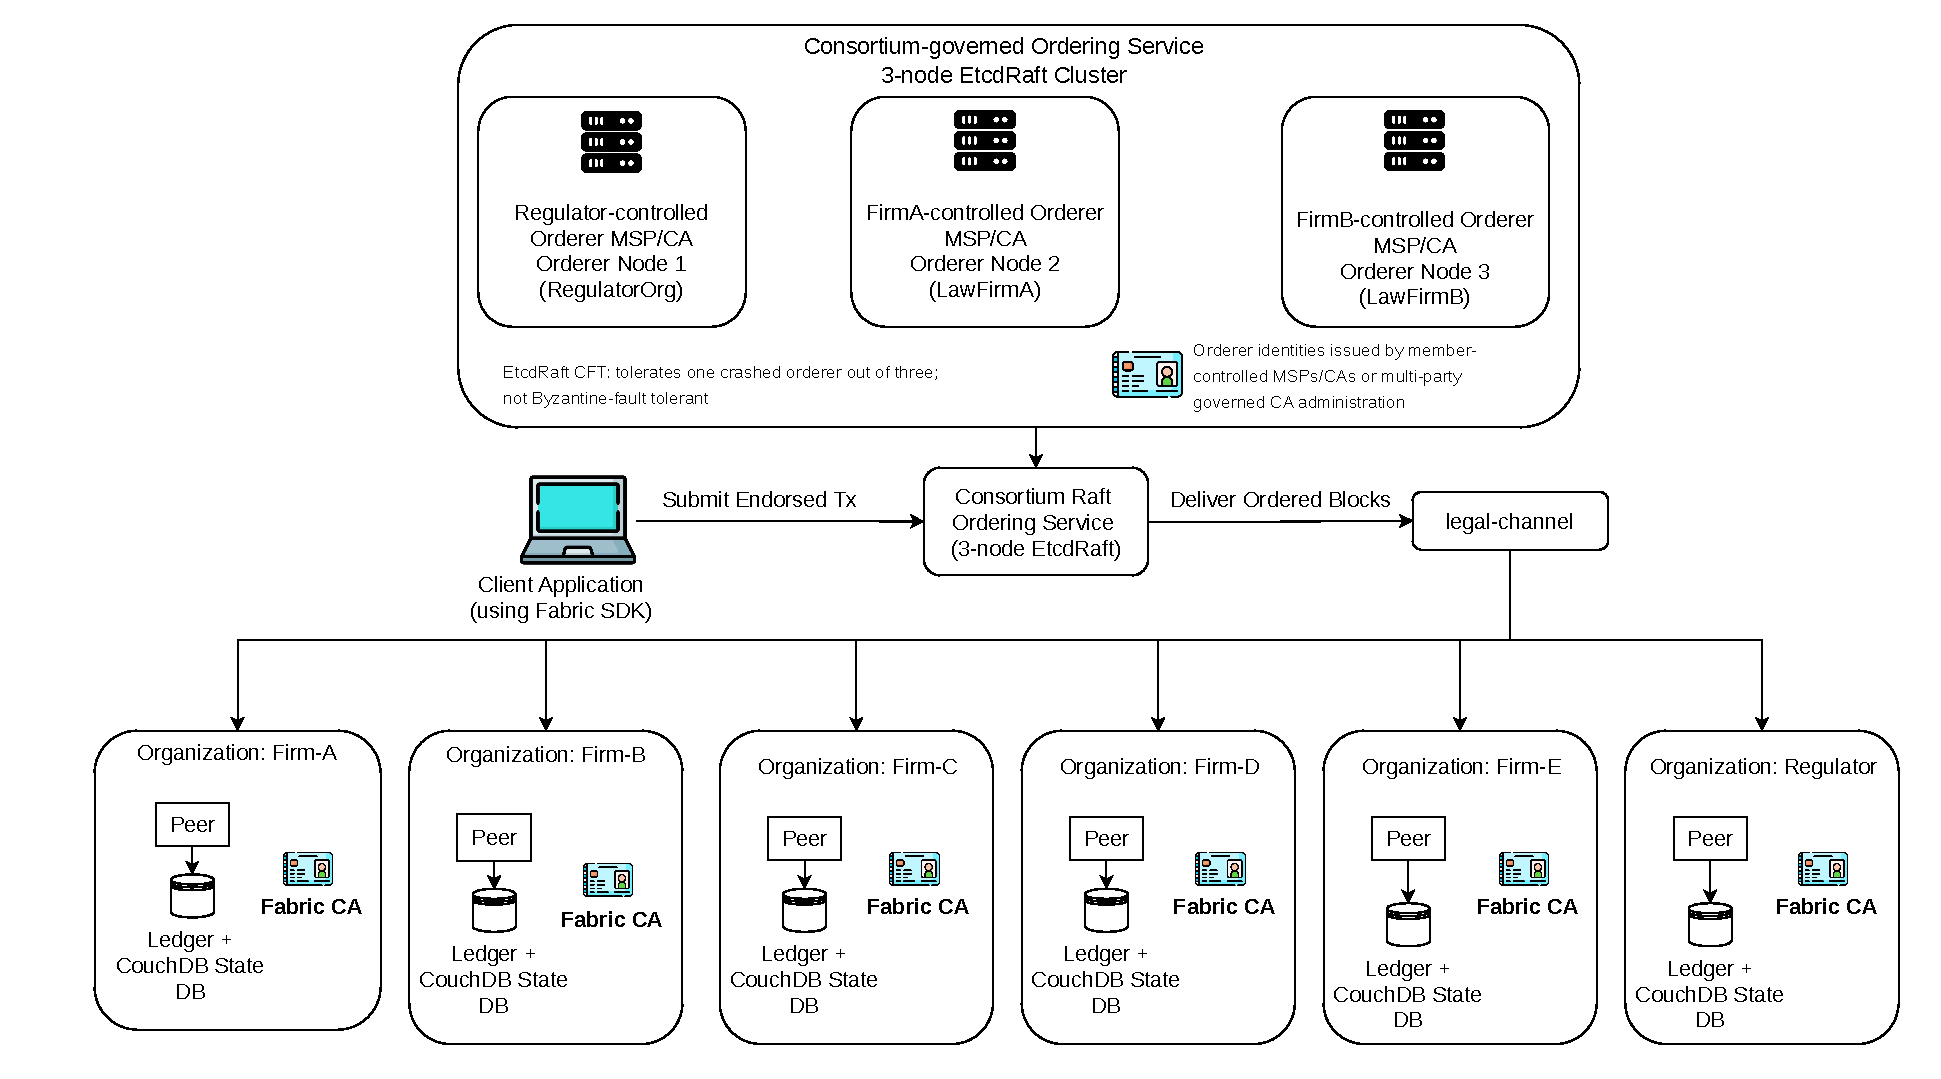
\includegraphics[width=2\columnwidth]{fabric_topology4.pdf}
    \caption{Six-peer-organization Fabric reference topology with a
consortium-governed three-node EtcdRaft ordering service. The orderer nodes
are operated by the regulator, FirmA, and FirmB under member-controlled
orderer identity administration or multi-party CA governance. Raft provides
crash-fault tolerance for one orderer failure; Byzantine-fault-tolerant
ordering is outside the prototype scope.}
    \label{fig:fabric_topology}
\end{figure*}

\subsection{Chaincode Design and Functionality}
\label{sec:chaincode}

The core business logic is encapsulated in the \texttt{legalcc}
chaincode, which implements: \texttt{RegisterDocument} (anchors
document hash, CID, and ECDSA signature as a ledger asset);
\texttt{GrantAccess} and \texttt{RevokeAccess} (manage capability
tokens with optional expiry in the on-chain ACL map);
\texttt{CheckAccess} (evaluates the on-chain ACL at query time with
time-bounded token enforcement; expiry write-back is omitted on the read
path to prevent MVCC read-write conflict crashes, as documented in
Listing~\ref{lst:checkaccess});
\texttt{GetHistoryForKey} (returns the full hash-linked transaction
history for any document key); and \texttt{CleanExpiredTokens}
(asynchronous administrative function that formally deprecates expired
grants in world state, invoked periodically via a background cron-job;
not required for authorization correctness, since \texttt{CheckAccess}
evaluates expiry dynamically at query time)~\cite{fabricChaincodeStubDoc}. Expiry
write-back is not relied on for authorization correctness: expired
grants are denied based on their \texttt{ExpiresAt} value. Concurrent
write-back behavior for the same expired grant was not isolated in
the experiment campaign and is treated as a production hardening
issue.

\subsection{Demonstration of Core System Workflows}
\label{sec:workflows_demo}

\subsubsection{Workflow 1: Granting Access Permissions}
Fig.~\ref{fig:grant_access_seq} shows the access grant sequence.
The document owner invokes \texttt{GrantAccess} through the frontend;
the application server relays to the chaincode, which writes the
time-bounded capability token to the ACL map in world state and emits
an \texttt{ACCESS\_GRANTED} audit event.

\begin{figure*}[!t]
    \centering
    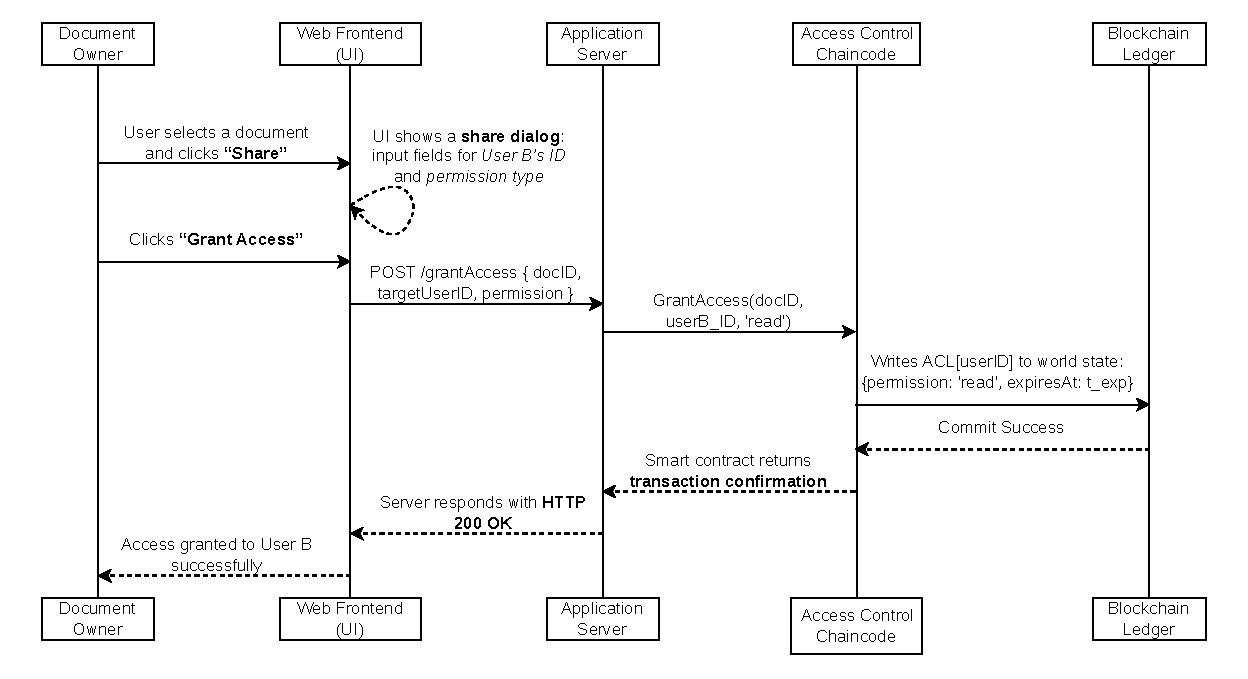
\includegraphics[width=0.82\textwidth]{grant_access_sequence.pdf}
    \caption{Sequence diagram for granting access permissions. The
    \texttt{GrantAccess} chaincode writes a time-bounded capability
    token to the on-chain ACL map, producing a ledger-verifiable record
    of the delegation.}
    \label{fig:grant_access_seq}
\end{figure*}

\subsubsection{Workflow 2: Verifying Access and Retrieving a Document}
Fig.~\ref{fig:verify_access_seq} illustrates the document retrieval
sequence. The application server enforces Layer~1 Spring Security
RBAC~\cite{RBACSandhu}, then invokes \texttt{CheckAccess} chaincode
(Layer~2). If both layers approve, the server retrieves the IPFS
ciphertext and returns it with the ECIES-wrapped key token for
client-side decryption.

\begin{figure*}[!t]
    \centering
    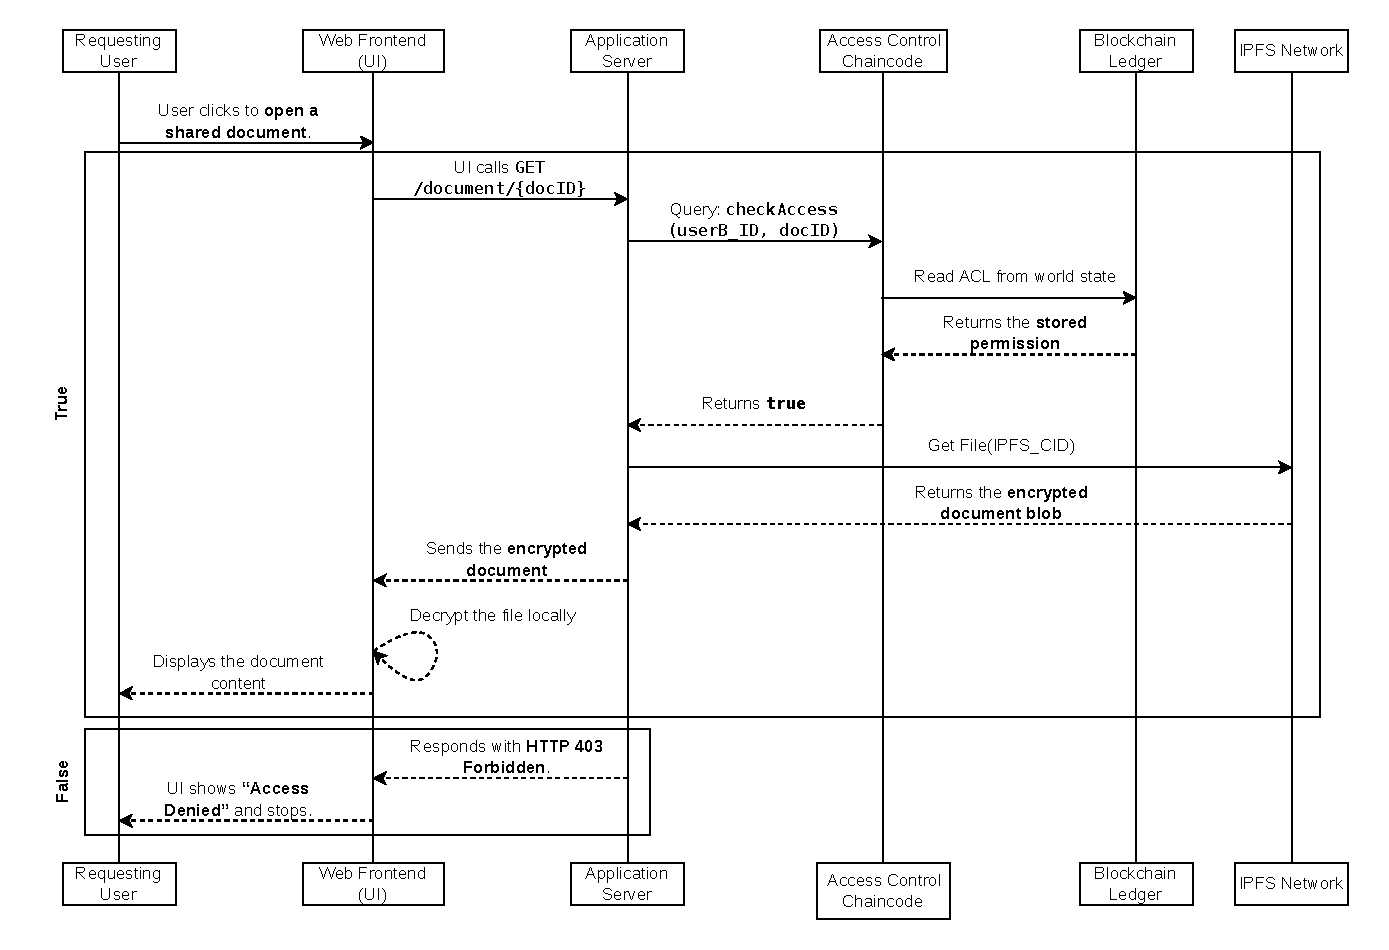
\includegraphics[width=0.88\textwidth]{verify_access_sequence.pdf}
    \caption{Access verification and document retrieval: Layer~1 (RBAC)
    and Layer~2 (\texttt{CheckAccess}) authorization, followed by
    ciphertext release on success or HTTP~403 denial on failure. Fail-closed
    handling of Fabric unavailability is shown separately in
    Fig.~\ref{fig:failclosed} and Listing~\ref{lst:download}.}
    \label{fig:verify_access_seq}
\end{figure*}

\subsubsection{Workflow 3: Activity Flow for Document Upload}
Fig.~\ref{fig:activity_diagram} presents the upload activity diagram.
In the framework design, encryption occurs client-side before the
application server forks two parallel threads: IPFS storage and
blockchain anchoring. A join node ensures both must complete before
confirmation is returned. The measured prototype fully implements the client-side encryption boundary;
the parallel fork/join thread model in this diagram is a framework-design
detail not independently validated in the experiment campaign.

\begin{figure*}[!t]
    \centering
    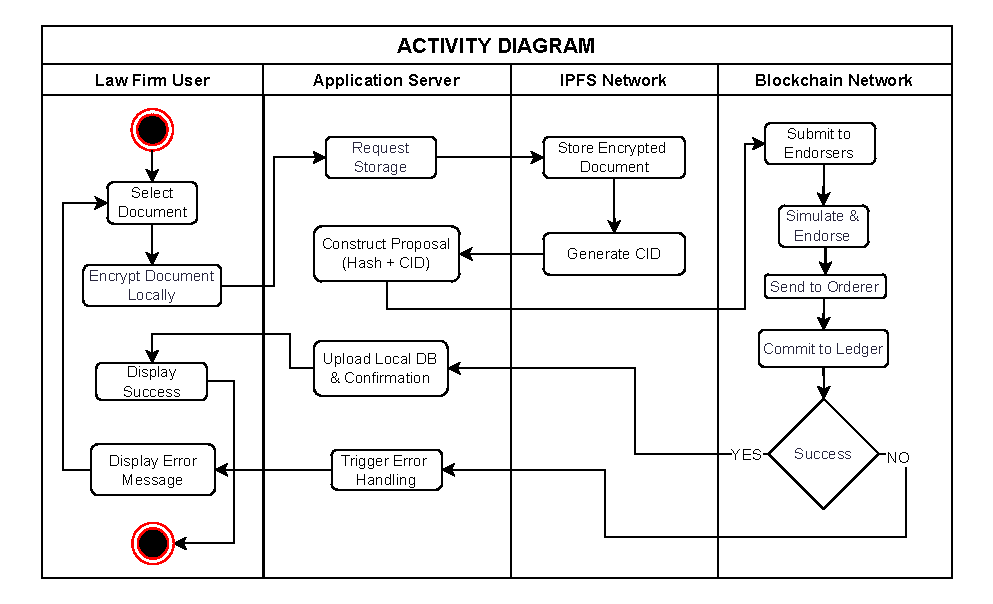
\includegraphics[width=1.4\columnwidth]{activity_diagram.pdf}
    \caption{Secure document upload and registration activity diagram.
    Strict client-side encryption is enforced before IPFS
    storage and blockchain anchoring proceed. The measured prototype
    fully implements this confidentiality boundary.}
    \label{fig:activity_diagram}
\end{figure*}


\subsection{User Interface and Functional Showcase}
\label{sec:ui}

The prototype exposes the full workflow through a web interface:
registration with role selection, a navigation dashboard, card-based case
management, and document dialogs that surface the content identifier,
Fabric transaction identifier, integrity hash, and wrapped-key reference
for each file, together with controls for downloading the encrypted
object or a locally decrypted copy. Because auditability is the central
claim of this work, Fig.~\ref{fig:ui_audit_views} shows the two
transparency views. The ledger explorer (Fig.~\ref{fig:ui_ledger_explorer})
groups recent entries by block and displays transaction IDs, channels,
timestamps, transaction types, and document references. The audit-log view
(Fig.~\ref{fig:ui_audit_log}) lists application events with timestamps and
expanded metadata so administrators can review user activity from within
the prototype interface. The remaining interface screenshots are provided
as supplementary material.

\begin{figure*}[!t]
\centering
\subfloat[Ledger explorer]{%
    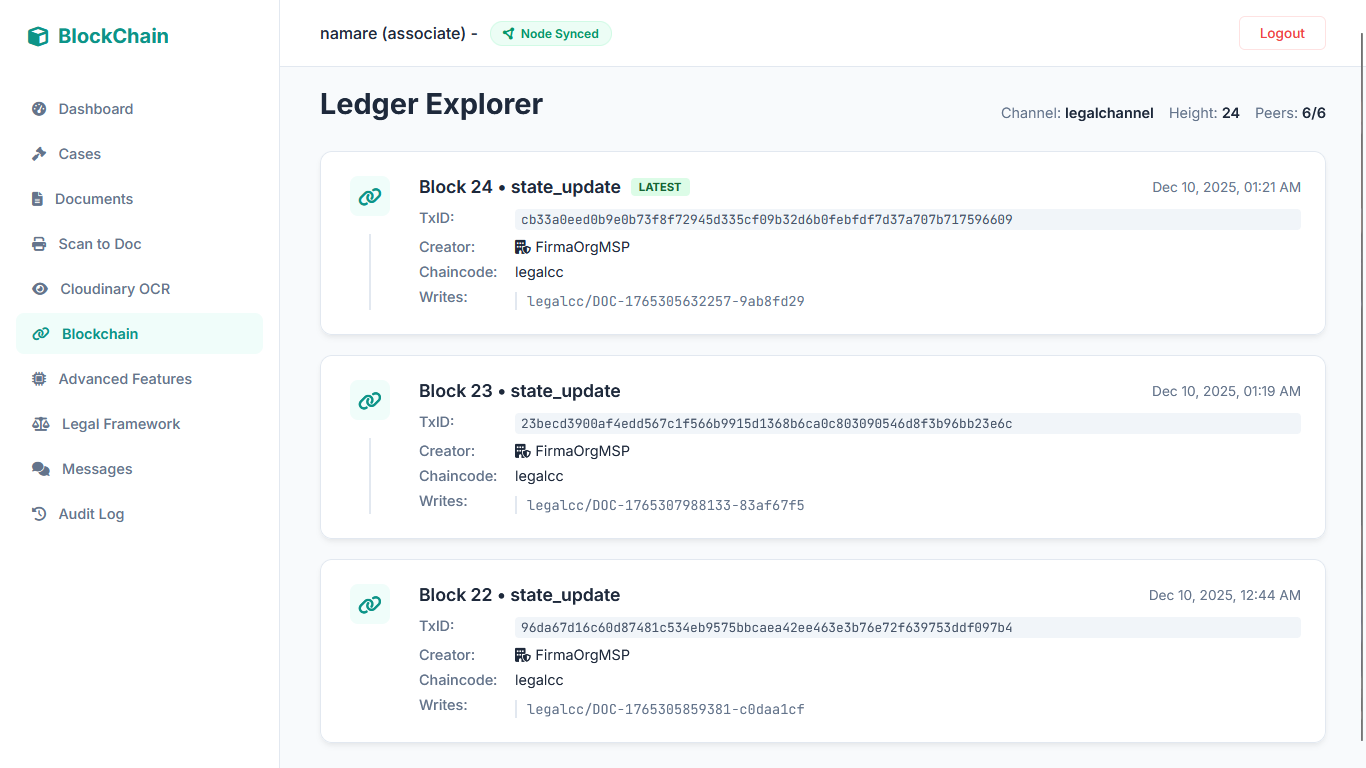
\includegraphics[width=0.48\linewidth]{ui_ledger_explorer.png}%
    \label{fig:ui_ledger_explorer}}\hfill
\subfloat[Audit log]{%
    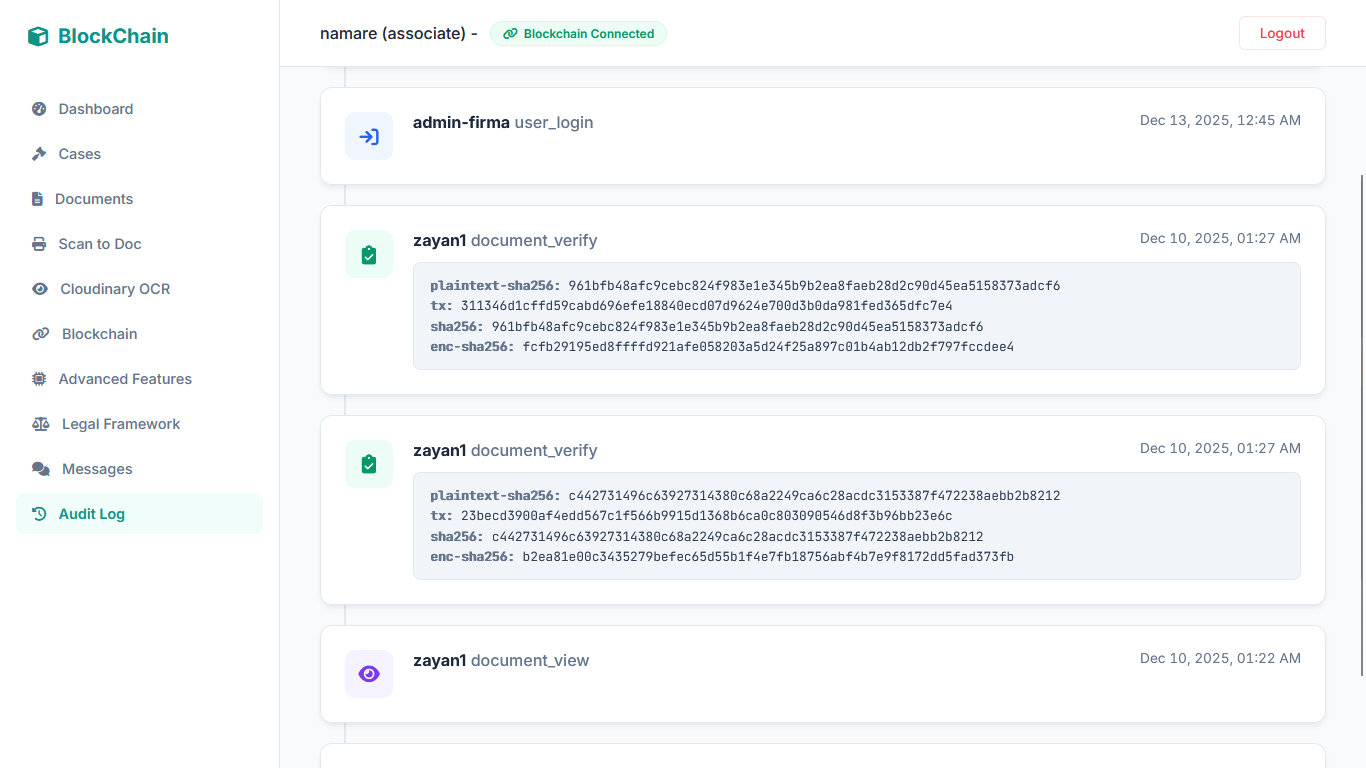
\includegraphics[width=0.48\linewidth]{ui_audit_log.png}%
    \label{fig:ui_audit_log}}
\caption{Audit and transparency views of the prototype interface.}
\label{fig:ui_audit_views}
\end{figure*}
% =========================================================================
% SECTION VI - PERFORMANCE EVALUATION
% =========================================================================

\section{Performance Evaluation}
\label{sec:performance}


Nine experiments evaluate RQ1–RQ3. Measurements were collected on
three platforms: a Windows~11 workstation (Ryzen~7~5700X,
Java~17~Temurin, Node.js~24), an Apple~M1 MacBook under Rosetta~2
emulation (macOS, Java~21~Temurin, Node.js~22), and a native
Linux~x86\_64 server (Intel Core Ultra~5~125H, Ubuntu~22.04,
8\,GB RAM, NVMe~SSD, Java~21~OpenJDK, Node.js~18). All authoritative
figures are from Linux; M1 and Windows results are auxiliary
cross-platform checks where reported.

The evaluated Fabric network used three peer organizations
(LawFirmA, LawFirmB, RegulatorOrg) on a shared \texttt{legalchannel},
each backed by CouchDB~3.2. The ordering service was a 3-node EtcdRaft
cluster across three distinct consortium members. This configuration
tolerates one crash fault under CFT assumptions, but the experiment
campaign did not evaluate Byzantine ordering behavior~\cite{hyperledgerFabricOrderingService_v24}.

Unless otherwise stated, \texttt{BatchTimeout} was set to 2\,s and
\texttt{BatchSize.MaxMessageCount} to 500. Sustained throughput was
measured with a 60\,s fixed-duration closed-loop load generator; a
fixed-count harness was used as a latency cross-check. A custom Node.js
harness targeted the Spring Boot REST gateway with a
20\,\%\,write\,/\,80\,\%\,read mix. Each data point is the mean of five
independent runs after a discarded warm-up round, following standard
Hyperledger Fabric benchmarking practice~\cite{caliper2021,woznica2022}.
Table~\ref{tab:hardware} summarizes the configurations.

Direct numerical comparison with prior systems is not possible because,
to the best of the authors' knowledge, the systems in
Table~\ref{tab:literature_review} do not report REST-gateway throughput
under concurrent load with a documented traffic mix~\cite{liu2024blockchain,twoLevelBlockchain,
onyeashie2025fabricEvidence,verma2021nyaya,hanafi2021ipfschain}. The
PostgreSQL-only baseline is therefore used as a reproducible upper-bound
reference~\cite{thakur2024}.

For upload-path experiments, the load generator submits opaque byte payloads
representing the IV-prepended ciphertext that the server receives in the
browser workflow. Consequently, Experiments~\hyperref[sec:exp_scalability]{1}--
\hyperref[sec:exp_filesize]{3} isolate REST-gateway, Fabric, database, and
IPFS costs; browser-side encryption is measured separately in
Experiment~\hyperref[sec:exp_crypto]{6}.

\begin{table}[!b]
\centering
\caption{Experimental Hardware Configurations}
\label{tab:hardware}
\renewcommand{\arraystretch}{1.2}
\begin{tabularx}{\columnwidth}{@{} l
    >{\raggedright\arraybackslash}X
    >{\raggedright\arraybackslash}X
    >{\raggedright\arraybackslash}X @{}}
\toprule
\textbf{Parameter} & \textbf{Windows} & \textbf{M1 (Rosetta)} &
\textbf{Linux (auth.)} \\
\midrule
OS      & Win 11 Pro       & macOS amd64 emu. & Ubuntu 22.04       \\
CPU     & Ryzen 7 5700X    & Apple M1         & Core Ultra 5 125H  \\
RAM     & 16\,GB           & 16\,GB           & 8\,GB            \\
Java    & 17 Temurin       & 21 Temurin       & 21 OpenJDK         \\
Fabric  & 2.4.x            & 2.4.x            & 2.4.x              \\
Orderer & 3-node Raft      & 3-node Raft      & 3-node Raft        \\
Role    & Auxiliary       & Exps.\,1--4      & Exps.\,1--9        \\
\bottomrule
\end{tabularx}
\end{table}

% -----------------------------------------------------------------
\subsection{Experiment~1: Scalability Under Concurrent Load}
\label{sec:exp_scalability}
% -----------------------------------------------------------------

This experiment varies concurrent client load from 50 to 600 and measures
committed throughput in both Fabric mode and a PostgreSQL-only baseline,
to answer RQ3. Writes were issued as \texttt{POST /documents/upload}
requests and reads as \texttt{GET /wrapped-key}, with a 10\,s per-request
timeout and five repetitions per concurrency level.

The framework REST gateway with Fabric sustained approximately
68--70\,TPS across the measured 50--600 client range, remaining
about 4.1 to $4.2\times$ above the synthetic baseline used as an illustrative capacity-planning assumption~\cite{aba2023,ilta2023} for a 1,000-user firm performing one document action per minute per user and showing zero transaction errors up to 400 clients. Throughput
is invariant with respect to concurrency: as load rises, per-request
latency grows while committed throughput holds flat, the signature
of a system gated by the fixed 2\,s Raft batch window rather than by
compute or concurrency. CPU utilization stayed below 23\,\% throughout confirming the bottleneck is the Raft orderer
\texttt{BatchTimeout=2s}, not compute. The PostgreSQL-only baseline
peaked near 279\,TPS in the stable region. Beyond that point,
the closed-loop load generator saturates, so the shaded region in
Fig.~\ref{fig:scalability} is treated as a client-side limit rather
than a database-server failure.

To evaluate operational viability, we establish a synthetic steady-state
baseline $1000/60 \approx 16.7$\,TPS. The sustained $\approx$68--70\,TPS
throughput provides a 4.2$\times$ safety margin over this average.

Three considerations bound this interpretation. First, the experiment used
the measured 3-organization deployment rather than the larger repository
topology. Larger deployments will incur additional gossip, endorsement, and
resource overhead, so the measured throughput is an upper bound for the
evaluated configuration rather than a guarantee for all consortium sizes.

Second, \texttt{BatchTimeout} is tunable. Reducing it from 2\,s to 500\,ms
raises the highest measured throughput to 193.0\,TPS under the evaluated
three-organization deployment, an 11.6$\times$ margin over the 16.7\,TPS
baseline without architectural change~\cite{hyperledgerFabricOrderingService_v24}.

Third, enterprise traffic is bursty. An aggressive $10\times$ burst factor
raises the target to $\approx$167\,TPS; Experiment~\hyperref[sec:exp_sensitivity]{8}
(Section~\ref{sec:exp_sensitivity}) shows that the 500\,ms setting reaches
193.0\,TPS, a 15.6\% margin above that peak target~\cite{benson2010network}.
The throughput cost of blockchain consensus is therefore a configuration
trade-off, not an architectural barrier.

\begin{figure*}[!t]
    \centering
    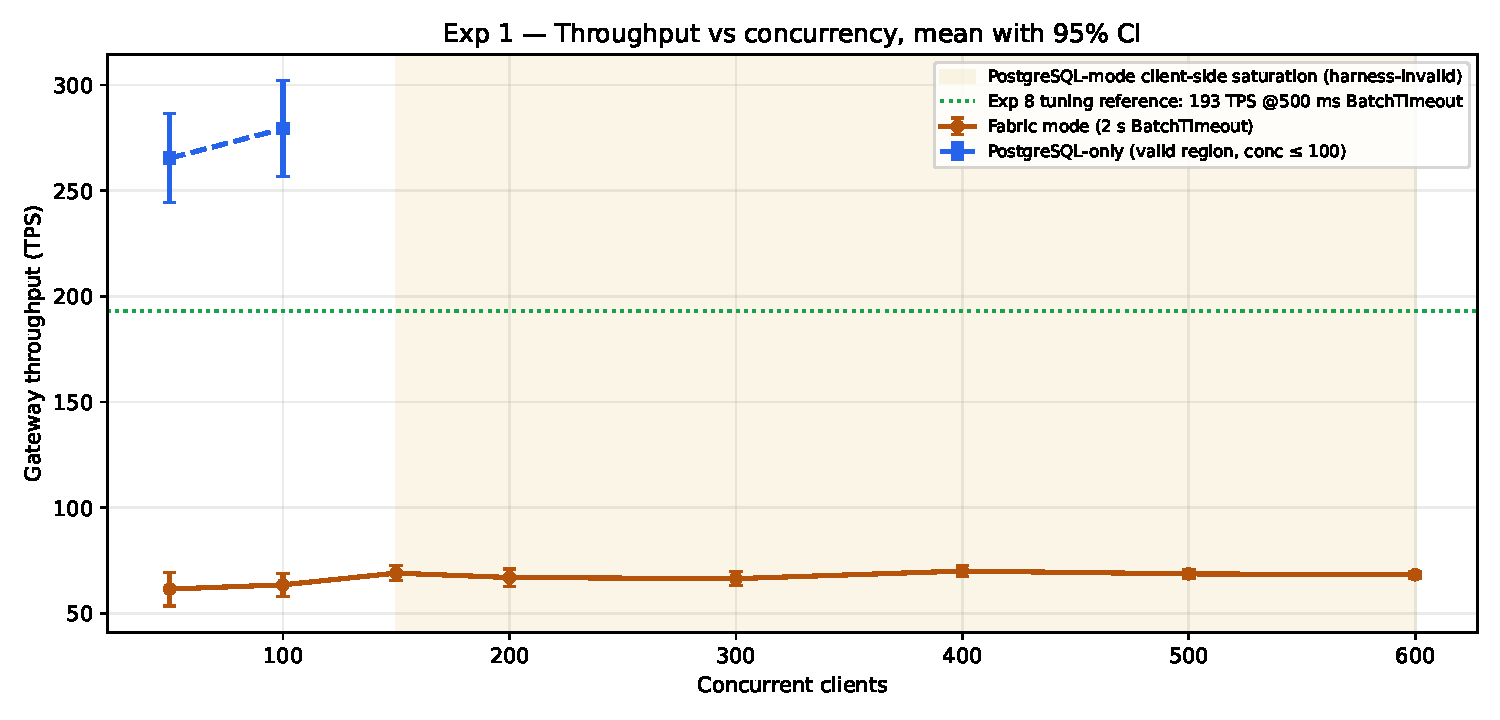
\includegraphics[width=0.78\textwidth]{fig1_scalability.pdf}
    \caption{Experiment~1 scalability under concurrent load on
    Linux~\texttt{x86\_64}: Fabric REST-gateway throughput compared with the
    PostgreSQL-only baseline, the client-side saturation region, and the
    Experiment~\ref{sec:exp_sensitivity} \texttt{BatchTimeout} tuning
    reference.}
    \label{fig:scalability}
\end{figure*}

% -----------------------------------------------------------------
\subsection{Experiment~2: Function-Level Operation Latency}
\label{sec:exp_latency}
% -----------------------------------------------------------------

This experiment isolates per-operation latency for \texttt{CheckAccess}
(read) and \texttt{RegisterDocument} (write) in Fabric and DB-only modes,
providing the direct answer to RQ2 and resolving the baseline inconsistency
cited in prior review.

\texttt{CheckAccess} latency was measured with a Node.js
\texttt{performance.now()} timer under sequential single-client load. Twenty
warm-up calls were discarded before 100 measured samples; the same protocol
was applied to the DB-only baseline on the same hardware. Warm-up matters
because JIT compilation can modestly overstate framework cost before the JVM
has stabilized.

\texttt{RegisterDocument} latency was measured end-to-end through the
Spring Boot Fabric gateway. The write path was verified to commit on-chain:
each call returned a real \texttt{fabricTxId}, and \texttt{GetDocumentHistory}
confirmed the same identifier. As with the read-path test, 100 measured
samples followed 20 warm-up calls.

The write path is dominated by ordering latency. \texttt{BatchTimeout}
accounts for $\approx$96\,\% of the 2{,}084\,ms total, and the independent
Experiment~\hyperref[sec:exp_filesize]{3} commit-latency constant (2{,}132\,$\pm$\,20\,ms across all
file sizes) is consistent with orderer processing dominating the path.
Experiment~\hyperref[sec:exp_latency]{2} and Experiment~\hyperref[sec:exp_filesize]{3} use independent sample sets and different
harness boundaries, so their values are reported as consistent observations
rather than additive components.

On native Linux~x86\_64 with JVM warm-up, Fabric access checks are
operationally indistinguishable from the DB-only path across the full
latency distribution (Table~\ref{tab:exp2dist}). Inter-quartile ranges
overlap, P99 differs by only 2.3\,ms, and a two-tailed Mann-Whitney $U$
test finds no statistically significant difference ($U = 4500.0$,
$p = 0.22$, $n = 100$ per path). Both paths remain below the 50\,ms
interactive threshold at all measured percentiles, including P99
(Fabric 15.5\,ms, DB-only 13.2\,ms). The slightly higher Fabric P99 is
consistent with occasional gateway scheduling jitter and does not affect
the threshold conclusion.

A standalone PostgreSQL-only write baseline was not collected because the
framework has no write path that bypasses Fabric. Measuring isolated
PostgreSQL inserts would omit the Fabric SDK endorsement round-trip and
orderer batch costs that are structurally part of every document
registration. The absolute \texttt{RegisterDocument} latency
(2{,}084\,ms P50) is therefore evaluated directly against the 5\,s SLO\@.
Experiment~\hyperref[sec:exp_scalability]{1} corroborates this interpretation: under the 68-70\,TPS Fabric
load, PostgreSQL operated at approximately 25\% of its independently
observed write-capacity reference ($\approx$279\,TPS), and CPU utilization
remained below 23\%. Cross-platform results also support BatchTimeout
dominance: the Apple~M1 session measured 2{,}147\,ms, within 3\,\% of the
Linux figure, as expected when the orderer timeout accounts for
$\approx$96\,\% of total write latency.

\begin{table}[ht]
\caption{Read-path latency distribution:
         \texttt{CheckAccess} via Fabric gateway
         vs.\ DB-only ACL lookup, warmed runs
         ($n = 100$ each, Linux x86\_64).}
\label{tab:exp2dist}
\renewcommand{\arraystretch}{1.15}
\begin{tabular}{lcc}
\hline
& \textbf{Fabric} & \textbf{DB-only} \\
\hline
Mean (ms)   & 7.293 & 7.548 \\
Std dev     & 2.352 & 2.092 \\
P25 (ms)    & 5.698 & 5.895 \\
P50 (ms)    & 6.510 & 7.162 \\
P75 (ms)    & 8.458 & 8.753 \\
P95 (ms)    & 10.871 & 11.283 \\
P99 (ms)    & 15.498 & 13.232 \\
\hline
\multicolumn{3}{l}{Mann-Whitney $U = 4500.0$,
  $p = 0.22$ (two-tailed); inter-quartile} \\
\multicolumn{3}{l}{ranges overlap; both
  paths ${<}$50\,ms at P99.} \\
\hline
\end{tabular}
\end{table}

The 0.65\,ms median difference between the Fabric and
PostgreSQL-only paths (Table~\ref{tab:exp2dist}) is statistically
insignificant, as shown above.
The absolute difference of 0.65\,ms is well within baseline
HTTP round-trip noise and meets the RQ2 read-overhead threshold
of 50\,ms with substantial headroom.
The write-latency SLO is met in absolute terms (2{,}084\,ms P50
vs.\ the 5\,s threshold); the incremental overhead of the Fabric path
over a PostgreSQL-only write was not separately measured, as no such
bypass path exists in the framework design.
Experiment~\hyperref[sec:exp_scalability]{1} confirms the latency is orderer-dominated rather than
database-dominated (PostgreSQL operating at $\approx$25\% of its
write-capacity reference, CPU below 23\%), so the SLO headroom is structurally
grounded, as summarized in Fig.~\ref{fig:latency}.

\begin{figure*}[!t]
    \centering
    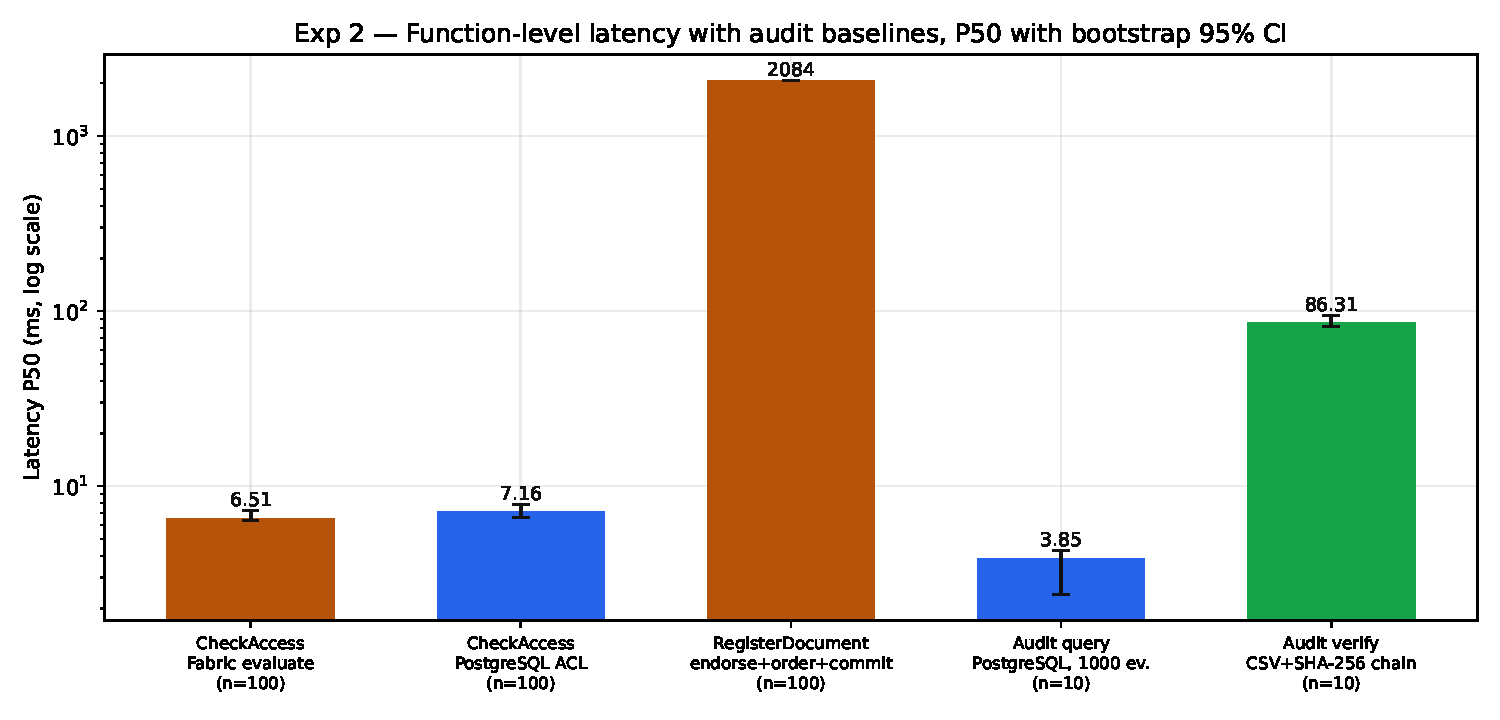
\includegraphics[width=0.78\textwidth]{fig2_latency.pdf}
\caption{Experiment~2 function-level latency (P50, log scale; Linux,
JVM-warmed, 100 samples): \texttt{CheckAccess}, \texttt{RegisterDocument},
and audit-query trust/latency baselines.}
    \label{fig:latency}
\end{figure*}

% -----------------------------------------------------------------
\subsection{Experiment~3: File-Size Independence of Ledger Latency}
\label{sec:exp_filesize}
% -----------------------------------------------------------------

Because the ledger stores only a fixed-length SHA-256 hash and IPFS CID regardless of document size, Fabric commit latency should be invariant with respect to payload size. This experiment confirms that property across a 1--50\,MB range. IPFS upload time was measured directly via the Kubo HTTP API (\texttt{curl} multipart, \texttt{pin=false}), isolating the IPFS-node upload cost from the secondary-pinning overhead present in the full REST path ($\approx$234\,ms on M1). Ten samples per file size were collected; total \emph{server-side} latency is Fabric constant plus IPFS upload. This excludes client browser encryption time and network transmission from the client to the REST gateway, which are workload- and bandwidth-dependent and not modelled in this experiment.

Fabric commit latency was 2,132\,$\pm$\,20\,ms across all file
sizes (1--50\,MB), flat within run-to-run Raft variance. IPFS upload grew
from 10\,ms at 1\,MB to 95\,ms at 50\,MB, consistent
with near-linear Kubo chunk hashing. Total server-side P50 ranged from
2,142\,ms to 2,226\,ms at 50\,MB, an $\approx$85\,ms increase over a 50$\times$ size range, entirely attributable to IPFS. All points remain below the 5\,s RQ2 threshold by more than 2$\times$, confirming that even large legal evidence files register without exceeding acceptable latency for a non-interactive background operation (Fig.~\ref{fig:filesize}).

\begin{figure*}[!t]
    \centering
    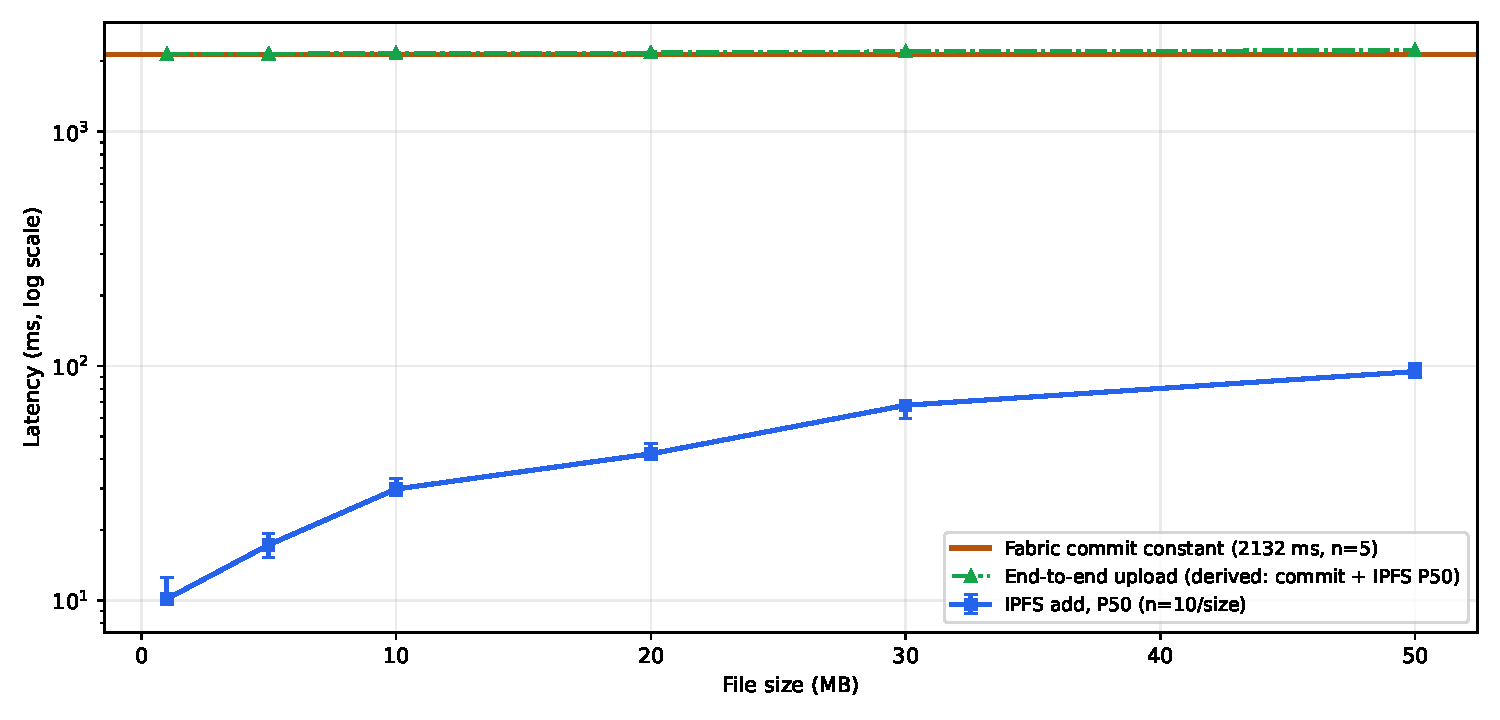
\includegraphics[width=0.78\textwidth]{fig3_filesize.pdf}
   \caption{Experiment~3 file-size independence of ledger latency (Linux,
   direct Kubo API), separating server-side P50, IPFS upload range
   (10--95\,ms), and constant Fabric commit latency.}
    \label{fig:filesize}
\end{figure*}

% -----------------------------------------------------------------
\subsection{Experiment~4: Audit Verification Efficiency}
\label{sec:exp_audit}
% -----------------------------------------------------------------

This experiment quantifies operational audit-query latency for PostgreSQL and CSV-based verification over 1,000 events, and compares those results with the Fabric \texttt{GetHistoryForKey} measurement from Experiment~\hyperref[sec:exp_gethistory]{7} at a 107-entry document history. These paths provide different trust guarantees and are not identical workloads: PostgreSQL is the low-latency operational index, CSV+SHA-256 is a manual verification baseline, and Fabric provides ledger-verifiable history. A PostgreSQL \texttt{audit\_log} table was seeded with 1,000 real Fabric-anchored events. Automated query time was measured via \texttt{GET /api/audit?size=1000} over five runs. Manual verification time was the wall-clock cost of a Python script that fetches the CSV export and recomputes the SHA-256 digest of each of the 1,000 exported records and cross-checks them against the on-chain validation anchors: a computational lower bound, since operational manual audit additionally requires human download, inspection, and cross-referencing.

The automated PostgreSQL query completed in 3.9\,ms median (mean 3.45\,ms; $n{=}10$ trials, conventional median as the average of the 5th and 6th sorted values). Manual script verification took 86.3\,ms,
22$\times$ slower in raw compute, and orders of magnitude
slower in practice. The raw speedup, however, is not the point. The architectural
contribution is the \emph{complementary independence} of the two stores.
PostgreSQL provides sub-5\,ms operational dashboards with
application/database-trigger-level append-only protection: row-level
triggers block UPDATE and DELETE; a
statement-level trigger blocks TRUNCATE (which bypasses row-level triggers
in PostgreSQL); and TRUNCATE privilege is revoked from all application
roles (Listing~\ref{lst:audittrigger}). The Fabric ledger provides
cryptographic non-repudiation that PostgreSQL cannot replicate: any
consortium peer can independently verify the complete audit trail via
\texttt{GetHistoryForKey} without trusting the application server or its
administrator~\cite{androulaki2018hyperledger, hyperledgerFabricOrderingService_v24}. Compromise of one store does not affect
the other. A malicious DB administrator who truncates the PostgreSQL log
leaves the on-chain Fabric record intact and independently verifiable, as compared in Fig.~\ref{fig:audit}.

\begin{figure*}[!tbp]
    \centering
    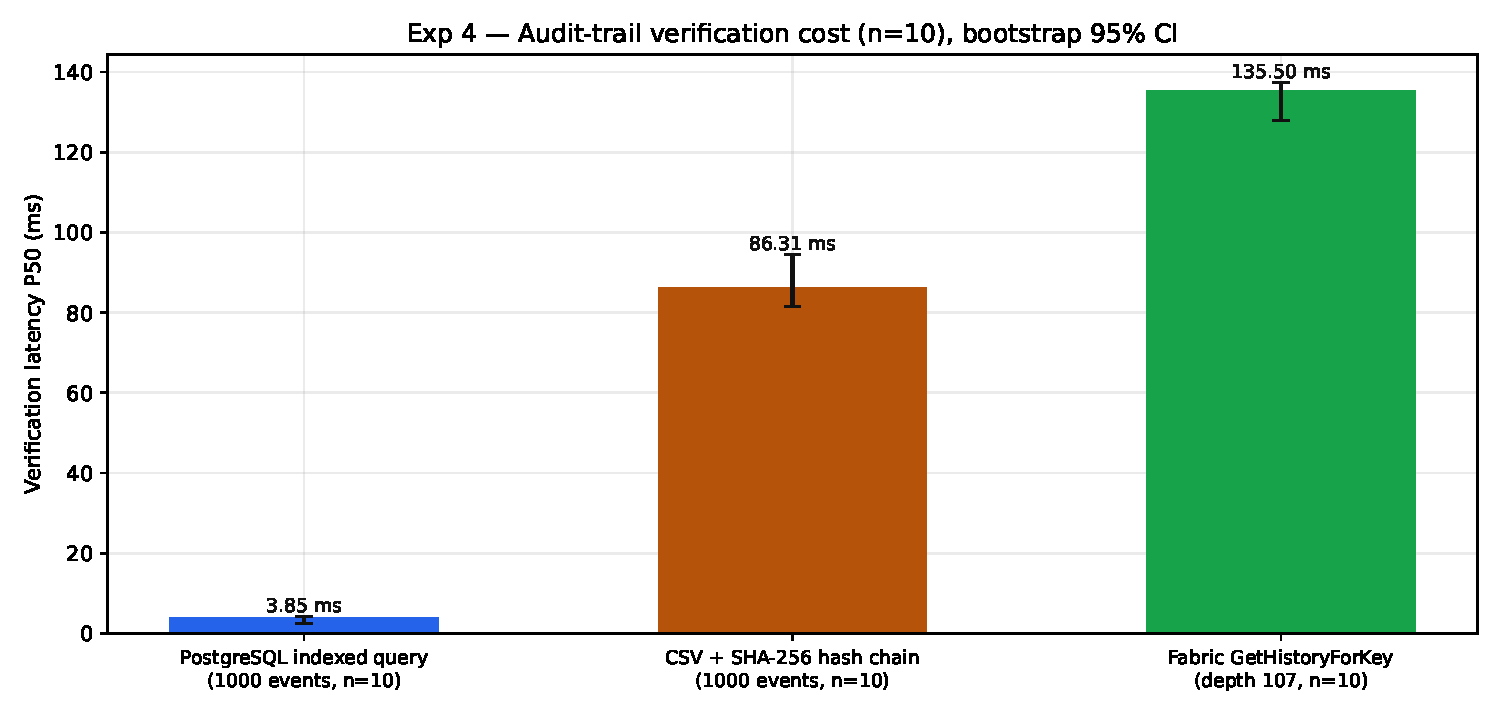
\includegraphics[width=0.86\textwidth]{fig4_audit.pdf}
    \caption{Experiment~4 audit verification efficiency across PostgreSQL
    queries, manual CSV\,+\,SHA-256 verification, and Fabric
    \texttt{GetHistoryForKey} ledger-verifiable history.}
    \label{fig:audit}
\end{figure*}

% -----------------------------------------------------------------
% -----------------------------------------------------------------
% -----------------------------------------------------------------
\subsection{Experiment~5: Resilience Under WAN Latency}
\label{sec:exp_wan}
% -----------------------------------------------------------------

WAN conditions were simulated in two configurations using Linux
\texttt{tc netem}. The first configuration injected symmetric delay
on the Docker bridge interface (\texttt{br-29a499b93a83}), affecting
host-to-container HTTP connections at 0, 50, 100, and 150\,ms RTT.
The second configuration additionally applied \texttt{tc netem} delay
to the \texttt{veth} interface of each orderer container, so that
inter-orderer Raft traffic also experienced the injected latency; this configuration was measured at all four RTT
levels. Throughput was measured at 200 concurrent clients (five
60-second trials per RTT level); commit latency was measured via 20
CLI samples of \texttt{RegisterDocument --waitForEvent} per level.

Bridge-only results (0--150\,ms RTT).
Throughput degraded from 68.2\,TPS at 0\,ms to 60.8\,TPS at 150\,ms RTT,
an 11.0\,\% reduction. It remained at least 3.6$\times$ above the
16.7\,TPS legal synthetic steady-state baseline at every tested level.

Commit latency grew from 2,140\,ms to 2,457\,ms (+317\,ms at 150\,ms RTT),
consistent with $\approx$2 HTTP round-trips through the injected delay. The
intermediate points (+100\,ms at 50\,ms RTT and +217\,ms at 100\,ms RTT)
confirm predictable growth. This configuration isolates HTTP-layer gateway
queuing because the injected delay does not reach container-to-container
Fabric peer traffic (Fig.~\ref{fig:wan}).

Bridge plus per-orderer-container results (0--150\,ms RTT).
With delay also applied to each orderer container's \texttt{veth} interface,
the 0\,ms baseline was 69.5\,TPS and 2,141\,ms P50 commit latency.
These values match the Fabric commit constant of 2,132\,$\pm$\,20\,ms from
Experiment~\hyperref[sec:exp_filesize]{3}.

Throughput declined to 50.9\,TPS at 50\,ms RTT,
47.0\,TPS at 100\,ms RTT, and 38.3\,TPS at 150\,ms RTT,
a 44.8\,\% total reduction from baseline. P50 commit latency grew
to 2,919\,ms (+778\,ms), 3,132\,ms (+991\,ms), and 3,588\,ms
(+1,447\,ms), respectively. The larger degradation relative to bridge-only
delay reflects Raft AppendEntries round-trip latency, now captured by the
per-container delay.

At the highest-RTT, most-delayed point, some requests exceeded the 10\,s
client timeout; reported TPS is therefore successful-commit throughput. Even
there, 38.3\,TPS remains 2.3$\times$ above the 16.7\,TPS baseline, and
3,588\,ms remains 1.4\,s below the 5\,s write budget. The threshold is not
approached anywhere in the tested range~\cite{hyperledgerFabricOrderingService_v24,thakkar2018performance}.
Table~\ref{tab:wan_comparison} summarizes both configurations.

\begin{table}[!t]
\centering
\caption{Experiment~\hyperref[sec:exp_wan]{5} WAN Resilience: bridge-only delay vs.\
bridge plus per-orderer-container \texttt{veth} delay (200 clients,
5 trials per RTT level).}
\label{tab:wan_comparison}
\renewcommand{\arraystretch}{1.2}
\small
\begin{tabularx}{\columnwidth}{@{} l
    >{\centering\arraybackslash}X
    >{\centering\arraybackslash}X
    >{\centering\arraybackslash}X
    >{\centering\arraybackslash}X @{}}
\toprule
\textbf{RTT} &
\multicolumn{2}{c}{\textbf{Mean TPS (200 clients)}} &
\multicolumn{2}{c}{\textbf{P50 Commit (ms)}} \\
\cmidrule(lr){2-3} \cmidrule(lr){4-5}
& Bridge & Bridge\,+\,veth & Bridge & Bridge\,+\,veth \\
\midrule
0\,ms   & 68.2 & 69.5          & 2,140 & 2,141 \\
50\,ms  & 64.9 & 50.9          & 2,240 & 2,919 \\
100\,ms & 62.3 & 47.0          & 2,357 & 3,132 \\
150\,ms & 60.8 & 38.3 & 2,457 & 3,588 \\
\bottomrule
\end{tabularx}
\end{table}

\begin{figure*}[!tbp]
    \centering
    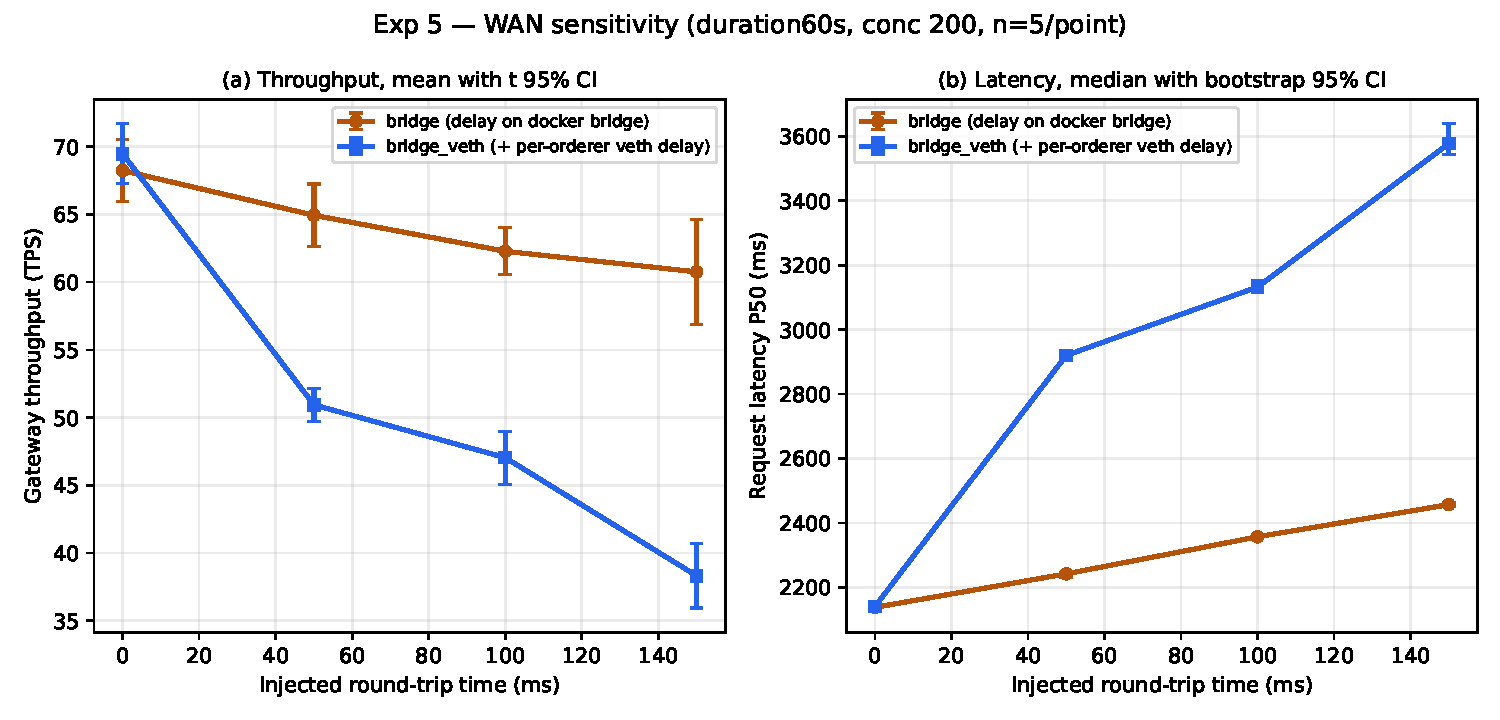
\includegraphics[width=0.94\textwidth]{fig5_wan.pdf}
    \caption{Experiment~5 WAN resilience (\texttt{tc netem},
    Linux~\texttt{x86\_64}, 200 clients), comparing bridge-only and
    bridge\,+\,\texttt{veth} delay effects on TPS and
    \texttt{RegisterDocument} latency.}
    \label{fig:wan}
\end{figure*}
% -----------------------------------------------------------------
\subsection{Experiment~6: Cryptographic Primitive Benchmark}
\label{sec:exp_crypto}
% -----------------------------------------------------------------

All cryptographic operations in the framework are intended to execute
client-side in the browser. Browser automation was unavailable in the
measurement environment, so this experiment uses Node.js WebCrypto as
a same-API fallback rather than claiming browser-performance results.
The benchmark was executed on Linux with Node.js WebCrypto and produced
170 CSV rows: 17 measured operation/configuration entries with 10
trials each. Fig.~\ref{fig:crypto} reports the operations most
relevant to the paper's document workflow. The goal is to verify that
password-based key derivation, document encryption, hashing, signing,
verification, and key wrapping are not the dominant costs in the
measured system.

PBKDF2-SHA256 at 600,000 iterations completed with a P50 latency of
100.44\,ms over 10 trials, within the 1,000\,ms
interaction budget commonly used for preserving user flow and
consistent with the work-factor guidance used in the
framework~\cite{nielsen1993usability,nist800132}. For 50\,MB inputs,
AES-256-GCM encryption measured 44.42\,ms P50,
AES-256-GCM decryption measured 61.94\,ms P50, and
SHA-256 hashing measured 44.43\,ms P50. These values confirm
that cryptographic processing is small relative to the Fabric write
latency dominated by the 2\,s \texttt{BatchTimeout}.

ECDSA~P-256 document signing and verification were sub-millisecond in
the same Node WebCrypto benchmark: signing measured
0.183\,ms P50 and verification measured
0.097\,ms P50. ECIES-style P-256 key wrapping measured
0.403\,ms P50 and unwrapping measured
0.603\,ms P50. ECIES is used primarily for compact
per-recipient token storage rather than for a speed advantage: both
ECIES and RSA wrapping costs are sub-millisecond in the Node WebCrypto
benchmark. The ECIES-style P-256 wrapped-key token occupies
125 bytes, compared with 256 bytes for
RSA-OAEP~2048, a 51.2\,\% reduction that directly reduces
ledger and network storage per access-grant event.

\begin{figure*}[!tbp]
    \centering
    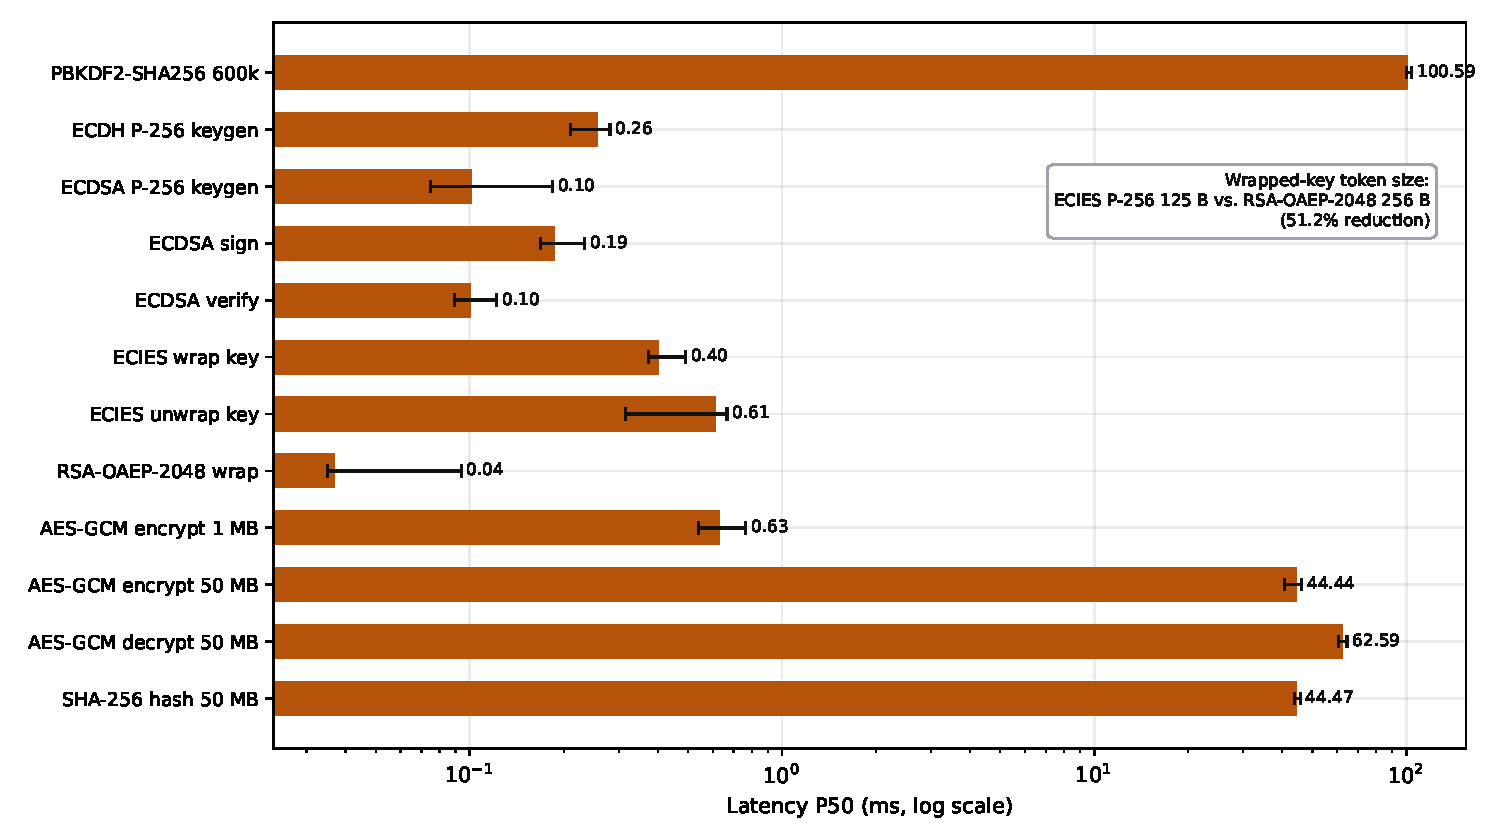
\includegraphics[width=0.90\textwidth]{fig6_crypto.pdf}
    \caption{Experiment~6 cryptographic primitive benchmark using Node.js
    WebCrypto fallback (Linux): PBKDF2-SHA256, AES-GCM, SHA-256, ECDSA,
    ECIES, and RSA-OAEP token-size comparison.}
    \label{fig:crypto}
\end{figure*}

% -----------------------------------------------------------------
\subsection{Experiment~7: Blockchain Audit Trail Query Depth}
\label{sec:exp_gethistory}
% -----------------------------------------------------------------

Experiment~\hyperref[sec:exp_audit]{4} showed that PostgreSQL serves operational dashboards at
3.9\,ms P50. The Fabric ledger's \texttt{GetHistoryForKey} path is slower,
but it is the only measured path that provides cryptographic
non-repudiation verifiable by any consortium peer. This experiment
therefore measures the cost of ledger-verifiable history queries at a
realistic workflow depth.

A benchmark document was seeded with 107 committed history entries:
one \texttt{RegisterDocument} transaction followed by 106
\texttt{GrantAccess} invocations, each committed in a separate block. This
depth represents an actively shared document with periodic access-grant
renewals across multiple firms. Ten trials were executed with
\texttt{peer chaincode query} (CLI), measuring the full round trip from peer
request, to CouchDB history scan, to response.

\texttt{GetHistoryForKey} completed in 135.5\,ms P50 (mean 134.0\,ms,
range 123--145\,ms, $\sigma = 6.1$\,ms). The coefficient of variation is
$<$5\,\%, indicating stable performance with no observed index-scan
anomalies. Because the audit-history measurement was obtained through a peer
chaincode query CLI path, whereas the main latency and throughput experiments
use the REST-gateway workload path, these measurements are reported as
distinct evaluation paths and should not be interpreted as identical
workloads. Only the 107-entry depth was directly measured.

CouchDB evaluates \texttt{GetHistoryForKey} with a full sequential scan and
no secondary index, so latency is expected to grow approximately linearly
with history depth. For that reason, the 1,000-entry value in
Fig.~\ref{fig:gethistory} is a back-of-envelope linear projection from the
single measured depth, not an independently measured point. Extrapolating
from 135.5\,ms at 107 entries gives $\approx$1,266\,ms at 1,000 entries.
That value is suitable for background forensic reports, but it exceeds the
200\,ms interactive threshold, which is crossed at approximately 158
entries. Multi-depth validation across deeper histories is left as future
work.

For documents with deeper histories, operational queries should use the
PostgreSQL \texttt{audit\_log} path measured in Experiment~\hyperref[sec:exp_audit]{4} (3.9\,ms P50).
The Fabric path is reserved for contexts requiring cryptographic
non-repudiation that no application-layer log can provide, and is the core
answer to RQ1~\cite{nistir8202,fabricChaincodeStubDoc}.

\begin{figure*}[!t]
    \centering
    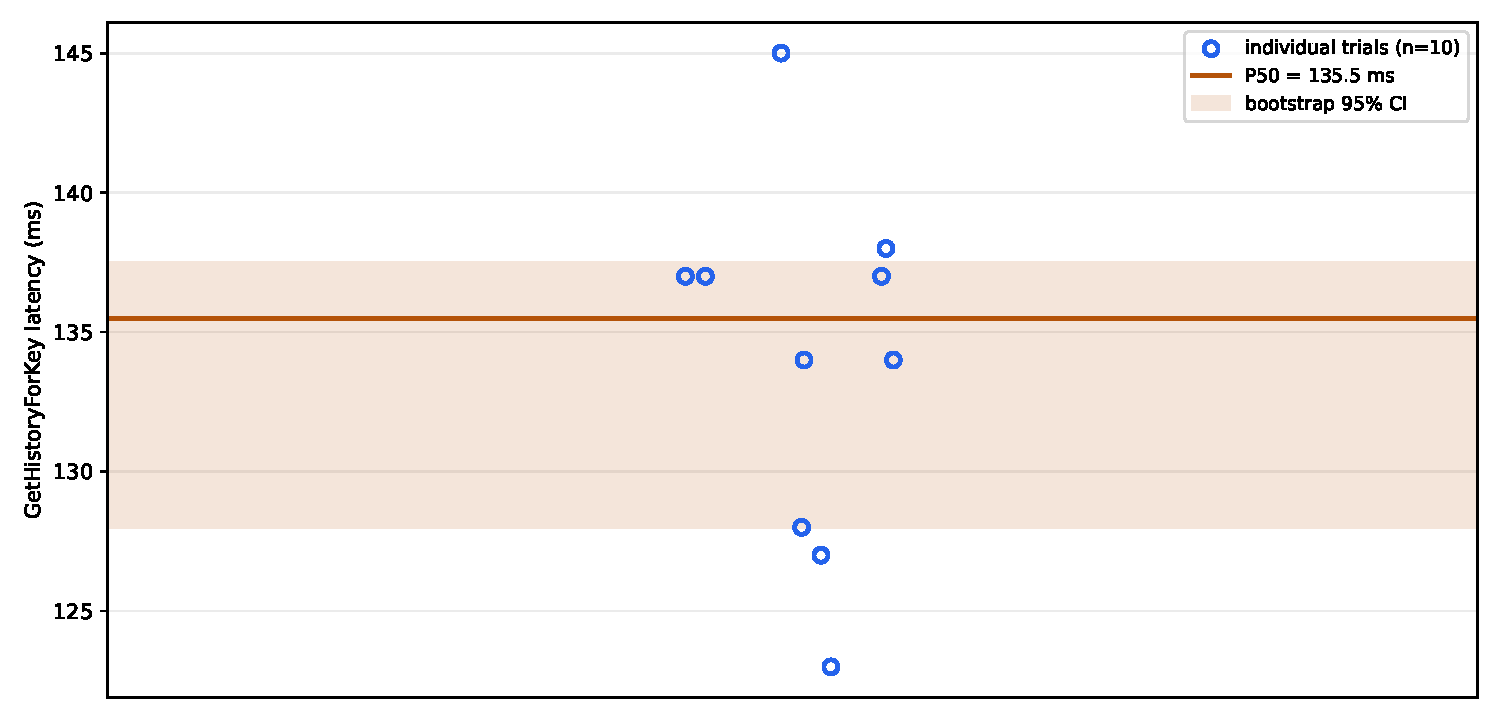
\includegraphics[width=0.78\textwidth]{fig7_gethistory.pdf}
    \caption{Experiment~7 Fabric \texttt{GetHistoryForKey} latency:
    107-entry history depth measured directly; deeper data points are linear
    projections from this single measurement, not independently measured
    values. Multi-depth validation is future work.}
    \label{fig:gethistory}
\end{figure*}

% -----------------------------------------------------------------
\subsection{Experiment~8: BatchTimeout Sensitivity}
\label{sec:exp_sensitivity}
% -----------------------------------------------------------------

Experiment~\hyperref[sec:exp_scalability]{1} established that throughput at the default
\texttt{BatchTimeout=2s} is gated by the Raft batch window rather than
by concurrency. This experiment characterizes the throughput--latency
trade-off as \texttt{BatchTimeout} is reduced, and tests whether the
load generator, not the orderer, becomes the limiting factor at
higher rates. At 50 concurrent clients, the network was rebuilt at
each of 2\,s, 500\,ms, and 250\,ms (\texttt{MaxMessageCount} fixed at
500), and ten 60-second sustained-throughput trials were taken per
setting using the closed-loop load generator. The load generator's own
CPU utilization was recorded each run to detect client-side
saturation.

Sustained throughput was 68--70\,TPS at 2\,s, rose to
193.0\,TPS at 500\,ms, and then fell to 180\,TPS at
250\,ms. The 500\,ms setting is therefore the sustained-throughput sweet
spot, providing an 11.6$\times$ margin over the 16.7\,TPS synthetic
steady-state baseline without architectural change.

The regression at 250\,ms is reproducible across all ten trials and is
\emph{not} a load-generator artifact. Client CPU remained far from
saturation: approximately 2\,\%, 11\,\%, and 14\,\% for the 2\,s, 500\,ms,
and 250\,ms settings, respectively. The likely cause is internal to the
orderer: a 250\,ms batch window cuts roughly twice as many small blocks as a
500\,ms window, increasing per-block commit and validation overhead. The
250\,ms setting also shows higher variance (137--206\,TPS across trials)
than 500\,ms (174--217\,TPS), slightly lowering net sustained throughput.

This resolves an apparent tool-dependent discrepancy. A fixed-count harness
ranks 250\,ms above 500\,ms because it favors per-request latency and batch
completion time. The sustained closed-loop measurement reported here is the
representative throughput metric and identifies 500\,ms as the operational
optimum shown in Fig.~\ref{fig:sensitivity}.

\begin{figure}[!t]
    \centering
    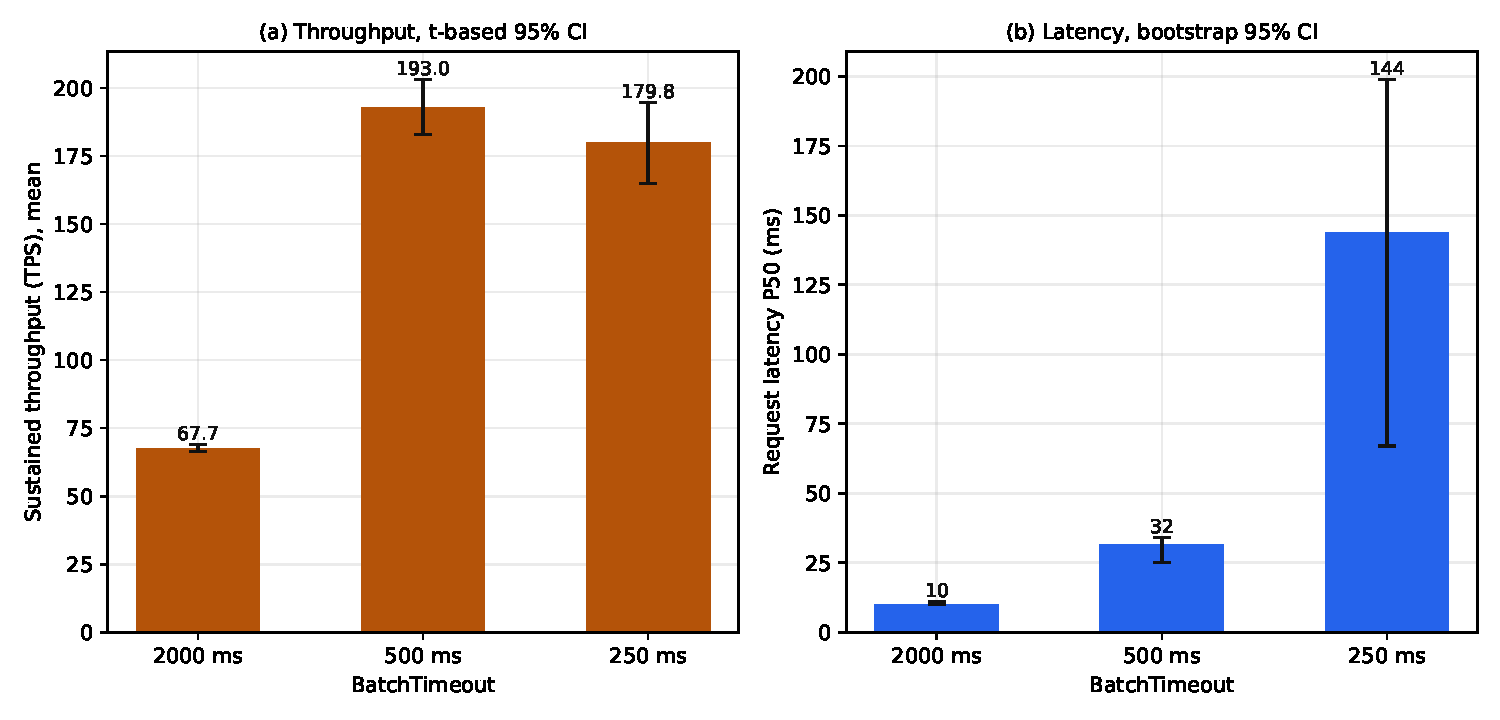
\includegraphics[width=\columnwidth]{fig8_sensitivity.pdf}
    \caption{Experiment~8 \texttt{BatchTimeout} sensitivity
    (Linux~\texttt{x86\_64}, 50 clients), showing default 2\,s, 500\,ms,
    and 250\,ms throughput with zero-error runs.}
    \label{fig:sensitivity}
\end{figure}

% -----------------------------------------------------------------
\subsection{Experiment~9: Fail-Closed Security Under Fabric Peer Outage}
\label{sec:exp_failclosed}
% -----------------------------------------------------------------

The threat model (Section~\ref{sec:threat_model}) specifies a strict \emph{fail-closed} architecture for protected document release during network partitions: if the Fabric peers become unreachable, the evaluated download path denies access rather than falling back to a database ACL. This experiment validates that behavior empirically. Under a steady 50-client ciphertext-download load, all three Fabric peers were stopped at $t = 30$\,s and restarted at $t = 75$\,s, a 45-second total Fabric peer outage. Fig.~\ref{fig:failclosed} shows the per-second timeline. Successful downloads dropped to exactly zero requests per second for the entire outage window; peers were restarted at $t = 75$\,s, with normal operation resuming automatically after an approximately 15-second gRPC reconnection lag. During the outage, the service sustained 25--45 HTTP~503 fail-closed denials per second, securely blocking all tested download requests (1,340 denial responses and 2,013 \mbox{PostgreSQL} audit rows; the difference reflects additional system-level audit events recorded per denial beyond the HTTP response itself). \texttt{FABRIC\_OUTAGE\_ACCESS\_DENIED} audit rows were written to the operational \mbox{PostgreSQL} log capturing the gRPC failure reason. On peer restart, normal Fabric evaluation resumed cleanly with no manual intervention.

This result substantiates the fail-closed behavior for the evaluated document-download path: a peer outage degrades to a secure denial state, prioritizing confidentiality over availability. A malicious DB administrator who deliberately induces an outage cannot force a fallback to the database ACL to bypass chaincode authorization on this path.

\begin{figure*}[!t]
    \centering
    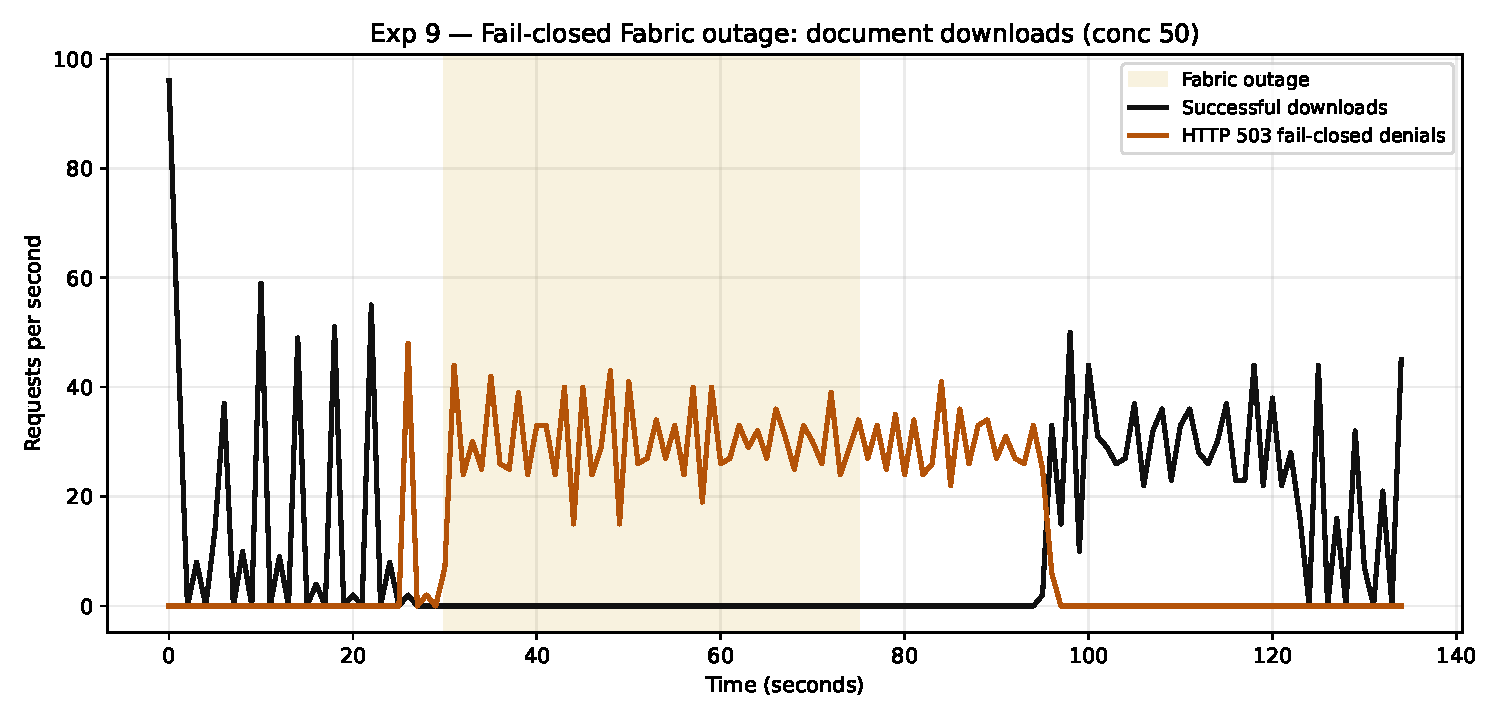
\includegraphics[width=0.85\textwidth]{fig9_failclosed_outage.pdf}
    \caption{Experiment~9 fail-closed Fabric peer outage: zero successful
    downloads during the 45\,s outage window; 1{,}340 HTTP~503 denial
    responses and 2{,}013 \mbox{PostgreSQL} audit rows (the difference
    reflects additional system-level audit events per denial); normal
    operation resumes after approximately 15\,s gRPC reconnection lag.}
    \label{fig:failclosed}
\end{figure*}
% =========================================================================
% SECTION VII --- LIMITATIONS AND FUTURE WORK
% =========================================================================
\section{Limitations and Future Work}
\label{sec:limitations}

\subsection{Limitations}
\label{sec:limitations_detail}

Each limitation is accompanied by a concrete mitigation path.


\begin{itemize}
\item \textbf{Coarse-grained intra-organization access control.}
The prototype \texttt{CheckAccess} chaincode (Listing~\ref{lst:checkaccess},
lines~37--39) grants read access to any peer whose MSP organization
matches the document owner's organization
(\texttt{doc.OwnerOrg == userOrg}), without requiring an individual
ACL entry. This constitutes an owner-org bypass: any member of
\texttt{LawFirmA} can access any document registered by any user in
\texttt{LawFirmA}. The framework design specifies per-user grants for
all principals; closing this gap in production requires removing the
organization-level fallback and enforcing explicit grants for
intra-organization peers, consistent with a zero-trust access model.

\item \textbf{Access-decision replay granularity.}
The \texttt{CheckAccess} chaincode uses the Fabric transaction timestamp
(\texttt{ctx.GetStub().GetTxTimestamp()}) for grant-expiry evaluation,
ensuring all endorsing peers assess the same proposal-embedded timestamp
regardless of local clock offset. Exact historical replay of individual
access decisions would additionally require committing each
access-decision event on-chain with its evaluated timestamp and result;
this is identified as a production hardening item and deferred to future
work. Expired-grant cleanup (as opposed to evaluation) follows a separate
eventual-consistency model via the asynchronous \texttt{CleanExpiredTokens}
job (Section~\ref{sec:chaincode}).
\end{itemize}

\subsubsection{Geographic Distribution and WAN Latency}
Experiment~\hyperref[sec:exp_wan]{5} evaluated WAN conditions up to 150\,ms RTT under two delay
configurations: bridge-only delay at the HTTP layer, and bridge plus
per-orderer-container \texttt{veth} delay, which also captures inter-orderer
Raft AppendEntries latency.

Under bridge-only delay, throughput degraded by 11.0\,\% (68.2 to
60.8\,TPS at 200 clients), and commit latency grew from 2,140\,ms to
2,457\,ms. When inter-orderer Raft traffic was also delayed, throughput
degraded by 44.8\,\% (69.5 to 38.3\,TPS), and commit latency grew from
2,141\,ms to 3,588\,ms. In both configurations, the 16.7\,TPS synthetic
steady-state baseline was cleared by at least 2.3$\times$, and commit
latency remained below the 5\,s operational threshold.

Performance in globally distributed, multi-continent deployments has not
been validated at production scale. Mitigations include reducing
\texttt{BatchTimeout} (500\,ms reached 193.0\,TPS and 250\,ms reached
180\,TPS in Experiment~\hyperref[sec:exp_sensitivity]{8}, both upper bounds for the evaluated
three-organization deployment) or placing orderer nodes with regional
awareness. Hyperledger Fabric's modular ordering service supports such
channel and placement choices~\cite{hyperledgerFabricOrderingService_v24,woznica2022}.

The WAN experiment also does not independently test orderer-node failover,
multi-peer failure combinations, or recovery during concurrent production-like
legal workloads. Likewise, the 16.7,TPS workload model is a synthetic
capacity-planning assumption rather than a replay of real legal transaction
logs. Future empirical work should replay anonymized legal document-management
transaction logs and test peer failure, orderer failover, and recovery under
geographically distributed load.


\subsubsection{Crash-Fault Tolerance vs.\ Byzantine Fault Tolerance}
The 3-node EtcdRaft ordering service provides CFT: it tolerates the
failure of any single ordering node. CFT does not protect against
Byzantine orderer behavior. In the proposed legal consortium, this
risk is mitigated architecturally: all ordering nodes are operated
by legally bound institutions under audited consortium agreements,
and Fabric's execute-order-validate pipeline ensures peers
independently validate every block regardless of orderer
behavior~\cite{androulaki2018hyperledger}. For deployments requiring
a stricter Byzantine threat model, Hyperledger Fabric~v3.0
introduces SmartBFT ordering as a production-hardening path that does
not change the document-management chaincode semantics, although it
does require ordering-service and channel-configuration changes~\cite{fabricWhatsNew3x,fabricOrderingServiceLatest,fabricBFTConfigurationDoc}.

\subsubsection{Key Management and Browser Dependency}
Three key management limitations arise. First, key rotation is
owner-initiated: re-encryption of all affected document keys after a
compromise requires the document owner's browser session. An interim
production-compatible direction is proxy re-encryption
(PRE), where an owner authorizes a proxy to transform a wrapped
document key from one recipient key to another without revealing the
document key to the proxy~\cite{ateniese2017redactable,nist80057,nist80053}.
This paper does not implement PRE; it is identified as a future
key-rotation mechanism that would require a careful construction,
threshold governance, and implementation-level security analysis. Second,
private keys are stored in browser \texttt{localStorage} under
PBKDF2-derived AES-256-GCM protection; key loss through browser data
clearing is permanent without a backup procedure. Third, all
cryptographic operations use the browser WebCrypto
API~\cite{w3cWebCrypto}, unavailable in headless or server-side
contexts. The production resolution for both the second and third
limitations is WebAuthn/FIDO2 or HSM-backed key protection, deployed
in a manner consistent with SP~800-63-4 AAL2/AAL3
requirements~\cite{nist800634,w3cWebAuthnL3,nist800131a,fips1403}.

\subsubsection{On-Chain Metadata Privacy}
Document content is protected by AES-256-GCM and is never stored on the
ledger. Metadata remains visible to channel members, including timestamps,
invoking MSP identity, CIDs, and access-event sequences. A channel member
can infer case activity patterns by observing transaction frequency and CID
patterns over time, even without decrypting content.

Hyperledger Fabric PDCs restrict sensitive fields to authorized subsets of
channel members~\cite{fabricPDCDoc,fabricChannelsDoc}. However, each
collection hash is still written to the main ledger~\cite{politou2019metadata}.
Possible mitigations include narrower channels or PDC scopes, metadata
minimization, batching, cover traffic, private access protocols, and
zero-knowledge proofs for selected policy checks~\cite{groth2016}.

The plaintext hash \(\mathcal{H}_D\) is also stored in main channel state.
Any peer holding a candidate document can therefore confirm its registration
without access to the ciphertext or decryption key. This leak is intentional
for the prototype's integrity-verification workflow, but production systems
should move \(\mathcal{H}_D\) into a Fabric Private Data Collection or
replace it with a keyed commitment available only to authorized auditors.

\subsubsection{Authentication Assurance Level}
The prototype implements AAL1 under NIST SP~800-63-4~\cite{nist800634}:
username/password with signed JSON Web Tokens~\cite{rfc7519jwt}.
AAL1 is adequate for the prototype evaluation of normal-path
chaincode access checks and audit mechanisms, but it is insufficient
for production legal consortium deployments. The authentication gateway is explicitly designed for
AAL2 and AAL3 upgrade without chaincode modification.

\subsubsection{Identity Database Public Key Integrity}

The PostgreSQL identity database stores each user's public keys (\texttt{pk\_ecies}, \texttt{pk\_sign}). The audit architecture protects the \texttt{audit\_log} table against modification, but the identity table is not subject to equivalent cryptographic protection. A database administrator with write access could substitute a malicious public key for a legitimate user's \texttt{pk\_ecies}; subsequent \texttt{GrantAccess} invocations would wrap $k_{enc}$ under the attacker's key and commit this subverted grant to the ledger as a valid transaction. The ledger would record a cryptographically correct but semantically compromised key exchange. The production mitigation is to anchor public key registrations to the Fabric ledger at enrollment time, for example by invoking a \texttt{RegisterIdentity} chaincode function that commits each user's public keys as a ledger asset, making any post-registration key substitution detectable by any consortium peer. This is deferred to future work alongside full per-user X.509 enrollment (Section~\ref{sec:future_work}).

\subsubsection{IPFS Retrieval Timeout and Thread Management}

The prototype does not enforce an explicit timeout on IPFS \texttt{GetFile} calls in the document download path. Under normal operation, the Fabric \texttt{CheckAccess} invocation completes before the IPFS retrieval begins. However, if the IPFS swarm experiences a node failure, disk fault, or network partition \emph{after} chaincode authorization succeeds, the Spring Boot HTTP thread handling the request may block indefinitely waiting for the ciphertext. Under sustained load, this could exhaust the application server's thread pool, causing a cascading failure that degrades or disables endpoints unrelated to IPFS. The production mitigation is a circuit-breaker pattern with a hard timeout (e.g., 5\,s) on all IPFS retrieval calls, returning HTTP~504 to the caller and logging an \texttt{IPFS\_RETRIEVAL\_TIMEOUT} audit event. This ensures IPFS unavailability degrades gracefully rather than propagating to a full service outage. Experiment~\hyperref[sec:exp_failclosed]{9} validates fail-closed behavior only for the document download path (\texttt{downloadCiphertext()}); the fail-closed behavior of the upload, grant, revoke, and audit-query paths is asserted by design (all paths invoke the same \texttt{FabricGatewayService} pattern and return \texttt{HTTP~503} on any \texttt{ServiceUnavailableException}) but was not independently validated empirically and is deferred to future work.

\subsubsection{GDPR and Regulatory Compliance}
\label{sec:gdpr}
The framework presents a structural tension with the European General
Data Protection Regulation (GDPR)~\cite{gdpr2016}. Article~17
grants data subjects a right to erasure, requiring personal data to
be deleted upon request. Hyperledger Fabric's append-only ledger
provides tamper-evidence precisely because committed transactions
cannot be deleted.

The proposed framework partially resolves this tension through design decomposition. Document content is stored off-chain in IPFS and can be unpinned and garbage-collected, effectively erasing the ciphertext from distributed storage~\cite{ipfsDocsQuickstartPin2025,ipfsDocsKuboGarbageCollection}. The on-chain ledger retains SHA-256 hashes, CIDs, timestamps, and MSP
identity references. Whether these values constitute personal data under GDPR Article~4(1)~\cite{gdpr2016} is context-dependent and legally contested.
Although hashes and CIDs cannot reconstruct the original document without the ciphertext and key, data-protection analysis often treats
cryptographic hashes of personal data as \emph{pseudonymised} rather
than anonymous, especially when linked to persistent institutional or user identities~\cite{finck2019blockchain,politou2019metadata}.

Article~17 compliance is therefore not fully solved by the prototype.
Off-chain erasure can remove encrypted document payloads from IPFS,
but append-only on-chain metadata may remain linkable to a person,
case, or institution depending on the deployment context. Production
use in jurisdictions applying GDPR erasure obligations requires a
deployment-specific legal basis and governance process, together with
technical hardening such as metadata minimization, narrower channels,
private data collections, off-chain redaction workflows, or
redactable-ledger mechanisms where legally required. Cross-jurisdiction data-residency obligations must also be resolved at
deployment time because the relevant legal exposure depends on where IPFS
pinning nodes, Fabric peers, and orderers are operated, and on which
jurisdictions treat on-chain hashes, CIDs, timestamps, or MSP identity
references as personal or regulated data.

Accordingly, the framework treats the ledger as evidentiary rather than dispositive: the consortium agreement, not the chaincode, remains the legal instrument governing access and erasure obligations. If on-chain metadata is treated as personal data in a deployment jurisdiction, full compliance may require a legal determination specific to the consortium or a technical mechanism for selective
record modification under governance. Redactable-blockchain mechanisms based on chameleon hashes are a possible research direction, but adopting them in Fabric would require modifying the block-hash construction and defining threshold governance for trapdoor use~\cite{ateniese2017redactable,lyons2018integration}. Without such advanced cryptographic deletion methodologies or explicit off-chain zero-knowledge verification patterns, the system may face significant compliance barriers to deployment in strict European jurisdictions handling personally identifiable legal records, a regulatory risk assessment consistent with EDPB guidance on pseudonymization and blockchain data governance~\cite{EDPB2025Pseudonymisation,Finck2020}.

\subsubsection{Integration with Legacy Legal Systems}
The prototype operates as a self-contained system. Production
deployment in an active legal consortium requires connectors to
existing practice management software, court filing platforms, and
document repositories. The following outlines the four architectural
concerns a production integration must address.

\textbf{(a) API surface and capability exposure.} The Spring Boot
REST gateway exposes four capability groups relevant to legacy
connectors: document registration (\texttt{POST /documents/upload}),
document retrieval (\texttt{GET /documents/\{id\}/download}), access
grant and revocation (\texttt{POST /documents/\{id\}/grant},
\texttt{POST /documents/\{id\}/revoke}), and audit trail query
(\texttt{GET /api/audit}). A legacy system with read-only audit
requirements needs only the last endpoint and does not interact with
the Fabric layer directly~\cite{springBoot325}.

\textbf{(b) Identity boundary: OAuth2 tokens to Fabric X.509
identities.} Legacy practice management systems typically issue
OAuth2 bearer tokens for authenticated sessions. At the integration
boundary, a token exchange service must map a validated OAuth2
identity to a Fabric X.509 certificate issued by the consortium
Fabric CA. In the prototype this mapping is handled under the shared
administrative MSP identity; in production each legacy user identity
must be enrolled with the Fabric CA and issued a certificate so that
chaincode invocations are attributable to a specific
principal~\cite{fabricCADoc,rfc7519jwt}.

\textbf{(c) Boundary security controls.} The integration boundary
must enforce: TLS mutual authentication (mTLS) between the legacy
connector and the Spring Boot gateway to prevent credential
interception; rate limiting on write endpoints to prevent batch
flooding of the Raft orderer beyond its \texttt{BatchTimeout}
capacity; and payload inspection to reject uploads that exceed the
IPFS node's configured maximum object size before a Fabric
transaction is attempted~\cite{nist80053}.

\textbf{(d) Phased migration path.} A four-phase migration is
recommended. Phase~1: read-only audit access, in which the legacy
system queries \texttt{GET /api/audit} to surface blockchain-verified
audit records alongside its existing log. Phase~2: read-write with
fallback, in which document registration and retrieval route through
the gateway but the legacy system retains its own ACL as a parallel
authority. Phase~2 is a pre-enforcement migration phase for
non-Fabric-classified documents only; once a document is classified as
Fabric-governed, its release path must not fall back to legacy ACL
authority. During Phase~2, legacy ACLs operate in shadow or advisory mode
alongside Fabric enforcement, not as an availability substitute. Phase~3: Fabric-governed ACL enforcement with fallback policy
disabled, in which the \texttt{CheckAccess} chaincode becomes the
access-control authority for protected document release and the
legacy ACL is retired. Phase~4: full per-user
X.509 enrollment, in which the shared administrative MSP identity is
replaced by per-user certificates and hardware-backed signing keys.
Each phase is independently deployable and requires no chaincode
modification~\cite{fabricChaincodeLifecycleDoc,nist80053}.

\subsection{Future Work}
\label{sec:future_work}
\label{sec:key_recovery_escrow}
\label{sec:regulator_interfaces}

Three directions dominate the path to production. First, per-user Fabric
CA enrollment with HSM-backed or WebAuthn/FIDO2 key
storage~\cite{fips1403,fabricCADoc,w3cWebAuthnL3} would replace the shared
administrative MSP identity and the password-protected
\texttt{localStorage} key store, closing the custodial-attribution gap
identified in Section~\ref{sec:prototype_scope}; the same infrastructure
supports a consortium-governed key-recovery workflow with KMS/HSM-backed
escrow, threshold administrative approval, and auditable re-wrapping of
recovered keys, so that no single administrator gains unilateral access to
user private keys. Second, formal verification of the \texttt{CheckAccess}
and \texttt{RegisterDocument} chaincode functions would provide
machine-checked guarantees of access-control completeness and absence of
chaincode-level bypasses under the modeled policy~\cite{permenev2020verx}.
Third, privacy-preserving access verification, including zero-knowledge
proofs for selected policy checks and batching or cover-traffic mechanisms
to reduce timing and frequency leakage, would address the on-chain
metadata exposure discussed in
Section~\ref{sec:limitations}~\cite{groth2016,fabricPDCDoc}.

Further directions include regulator-facing compliance interfaces
(read-only audit dashboards and joint endorsement policies such as
\texttt{AND('LawFirmAMSP.peer', 'RegulatorMSP.peer')}), real-time anomaly
detection over the low-latency audit feed~\cite{siddamsetti2024anomaly},
decentralized identity integration bridged to Fabric MSP
enrollment~\cite{sporny2023did}, cross-network evidence verification via
relay mechanisms or verifiable credentials~\cite{sporny2022vc},
cross-version CID chaining for document-version provenance, formal
incentive mechanisms for private-swarm pinning, and a comparative
complexity and cost model spanning application-only, append-only database,
audit-log, and on-path authorization architectures.
% =========================================================================
% SECTION VIII --- CONCLUSION
% =========================================================================
\FloatBarrier
\section{Discussion}
\label{sec:discussion}

This section interprets the experimental results in relation to the three
research questions and clarifies the boundaries of the measured prototype.
The framework combines Hyperledger Fabric, encrypted IPFS storage, and a
REST-based application gateway. Its central contribution is not a new
access-control primitive, not a Byzantine-fault-tolerant ordering protocol,
and not a production-ready legal deployment. Instead, the work evaluates the
practical effect of moving the document-release authorization boundary from
application-only trust to ledger-verifiable access-control state on the
normal release path, with fail-closed behavior empirically confirmed for the
download path. The prototype still has explicit boundaries, including
server-managed Fabric MSP credentials and a two-node private IPFS swarm, but
it implements strict client-side encryption and, on the evaluated
document-download path, a fail-closed security policy during Fabric
unavailability.

\textbf{RQ1} asked whether a permissioned blockchain architecture can make
legal-document access decisions and audit events independently verifiable
while preserving confidentiality during Fabric unavailability. The answer is
affirmative within the evaluated scope. Access-control \emph{state}, namely
grants, revocations, and document registrations, is independently
verifiable by consortium peers. \texttt{CheckAccess} derives each download
decision from that state at request time, although individual query results
are not themselves committed as transactions.

This result has two important boundaries. First, ledger transactions remain
attributable to the prototype's server-managed MSP identity until per-user
Fabric CA enrollment is implemented (Table~\ref{tab:framework_vs_prototype}).
Second, per-user \texttt{CheckAccess} enforcement was demonstrated for
cross-organization access. Intra-organization access still falls back to
organization-level membership; removing that fallback is the primary
production hardening step.

The dual-store audit design separates operational speed from independent
verifiability. PostgreSQL provides low-latency operational audit queries
(3.9\,ms P50 for 1,000 events, Experiment~\hyperref[sec:exp_audit]{4}). Fabric
\texttt{GetHistoryForKey} provides ledger-verifiable history (135.5\,ms P50
at a 107-entry document history, Experiment~\hyperref[sec:exp_gethistory]{7}).
The 107-entry history is shallow relative to production legal lifecycles, so
deeper-history scaling remains future work.

Under the stated threat model, a malicious database administrator cannot
silently rewrite Fabric history. A compromised IPFS node also cannot
undetectably modify document ciphertext because $\mathcal{H}_D$ is anchored
on-chain at registration. During Fabric peer outages, the evaluated download
path denied all downloads and logged \texttt{FABRIC\_OUTAGE\_ACCESS\_DENIED}
events to the operational \mbox{PostgreSQL} audit log. Anchoring those outage
denials on Fabric would require queue-and-replay support.

\textbf{RQ2} asked whether chaincode-based access evaluation adds acceptable
overhead for interactive legal workflows. The read-path threshold is met.
Fabric \texttt{CheckAccess} and the PostgreSQL-only ACL baseline are
statistically indistinguishable (6.51\,ms vs.\ 7.16\,ms P50, Mann-Whitney
$U{=}4500.0$, $p{=}0.22$, $n{=}100$), and both remain below 15.5\,ms at P99.

The write-latency \textsc{SLO} is also met in absolute terms:
\texttt{RegisterDocument} measured 2{,}084\,ms P50 against the 5\,s threshold.
The incremental overhead over a PostgreSQL-only write was not measured
because the framework has no database-only registration path.
Experiment~\hyperref[sec:exp_scalability]{1} indicates that latency is
orderer-dominated rather than database-dominated, with PostgreSQL at
$\approx$25\% of its write-capacity reference and CPU below 23\%.

File-size experiments show that Fabric commit latency is independent of
payload size because the ledger stores only metadata, hashes, and CIDs. WAN
experiments further show that, even with 150\,ms RTT applied to inter-orderer
Raft traffic, throughput remains above the estimated workload and write
latency remains below 5\,s. The file-size experiments report server-side P50;
client-side AES-256-GCM encryption adds approximately 44\,ms P50 for a 50\,MB
input, as measured in Experiment~\hyperref[sec:exp_crypto]{6}.

\textbf{RQ3} asked whether the framework sustains throughput sufficient for
realistic legal workload peaks. The measured REST-gateway Fabric deployment
sustains approximately 68--70\,TPS across 50--600 concurrent clients, about
4.2$\times$ above the estimated 16.7\,TPS workload for a 1,000-user
organization issuing one document action per minute per user. Reducing
\texttt{BatchTimeout} to 500\,ms produced the highest measured throughput,
193.0\,TPS, under the evaluated three-organization deployment, an
11.6$\times$ margin without changing the application architecture.

Experiment~\hyperref[sec:exp_failclosed]{9} confirms strict fail-closed
enforcement on the document-download path. Successful downloads fell to
exactly zero for the full 45-second Fabric unavailability window, while
HTTP~503 denials continued at 25--45 per second. Every denied attempt was
recorded in the operational \mbox{PostgreSQL} audit log, consistent with the
outage-anchoring limitation noted under RQ1.

Normal operation resumed automatically after an approximately 15-second gRPC
reconnection lag. The upload, grant, revoke, and audit-query paths enforce the
same policy by design through the same \texttt{FabricGatewayService} pattern,
but were not independently validated in the experiment campaign and are
identified as future empirical work.

The evaluation also shows that the cryptographic layer is not the dominant
performance cost. Using Node.js WebCrypto as a same-API fallback,
PBKDF2-SHA256 at 600,000 iterations measured 100.44\,ms P50, AES-GCM
encryption of a 50\,MB document measured 44.42\,ms P50, and AES-GCM
decryption measured 61.94\,ms P50. ECDSA signing and verification, and ECIES
wrapping and unwrapping, were sub-millisecond in the measured environment.
ECIES-style P-256 is used primarily for compact per-recipient key
distribution: its 125-byte wrapped-key token is 51.2\,\% smaller than the
256-byte RSA-OAEP~2048 token.

\FloatBarrier
\section{Conclusion}
\label{sec:conclusion}

This paper presented a hybrid framework for legal document management that
combines Hyperledger Fabric, encrypted IPFS storage, and a REST-based
application gateway. The core contribution is an empirical systems baseline
for moving legal-document release decisions from application-only
authorization to Fabric-backed \texttt{CheckAccess} evaluation on the normal
download path. The work does not claim to introduce a new access-control
primitive, a Byzantine-fault-tolerant ordering protocol, or a production-ready
legal deployment.

The results show that this design can provide ledger-verifiable
access-control state while maintaining practical performance for interactive
legal workflows. Fabric access checks were statistically indistinguishable
from the PostgreSQL-only ACL baseline on the evaluated read path, and the
REST-gateway Fabric deployment sustained throughput above the estimated
workload baseline. The fail-closed outage experiment further showed that
successful downloads fell to zero during Fabric unavailability, confirming
the evaluated download path's strict denial behavior.

These results substantiate the contributions set out in
Section~\ref{sec:contributions}: a measured relocation of the enforcement
boundary to ledger-verifiable access-control state, chaincode-enforced
time-bounded grants and revocation, a dual-store audit design separating
low-latency operational queries from ledger-verifiable history, and a
nine-experiment evaluation spanning throughput to fail-closed outage
behavior.

Table~\ref{tab:framework_vs_prototype} documents the gaps between framework
design and current implementation, bounding the measured prototype relative
to the framework design. To the best of the authors' knowledge, none of the
prior Fabric\,+\,IPFS legal-document systems in Table~\ref{tab:literature_review}
report the latency cost of placing \texttt{CheckAccess} on the critical
download path; the closest measurement is the 146--156\,ms end-to-end
retrieval authorization that RBAC-IPFS reports for generic file sharing
under an emulated 50\,ms wide-area network~\cite{liu2026rbacipfs}, which
is complementary to, but not directly comparable with, the LAN-scale
function-level isolation reported here. The negligible read overhead
measured here (6.51\,ms vs.\ 7.16\,ms P50, a 0.65\,ms difference,
$n{=}100$) confirms that this architectural choice imposes negligible
interactive overhead. It also establishes a reproducible baseline
against which future on-path enforcement designs can be evaluated.

Future work will focus on per-user Fabric CA enrollment, HSM/WebAuthn-backed
key protection, privacy-preserving access verification, formal verification
of chaincode policy logic, stronger IPFS persistence governance, and
compliance mechanisms for jurisdictions where append-only on-chain metadata
raises erasure or data-protection concerns.


\appendix
\section{Implementation listings}
\label{app:listings}

This appendix collects the implementation listings referenced in the main
text: browser-side encryption and key derivation, server-side signature
verification, the fail-closed download path, and the audit-log trigger
schema.

\begin{lstlisting}[language=TypeScript,
    caption={Browser AES-256-GCM document encryption. Fresh 256-bit
    key and 96-bit IV generated per document via
    \texttt{window.crypto.getRandomValues}. SHA-256 hash computed of
    plaintext \emph{before} encryption. Server receives only
    IV-prepended ciphertext.},
    label=lst:encrypt]
// frontend/src/lib/crypto.ts
export async function encryptDocument(
    file: ArrayBuffer
): Promise<EncryptedDocument> {
  const key = await subtle.generateKey(
      { name: 'AES-GCM', length: 256 },
      true, ['encrypt','decrypt'])
  const iv = crypto.getRandomValues(new Uint8Array(12))
  const [ciphertext, plainHashBuffer, rawKey] = await Promise.all([
    subtle.encrypt({ name: 'AES-GCM', iv }, key, file),
    subtle.digest('SHA-256', file),  // Plaintext hash
    subtle.exportKey('raw', key),
  ])
  // Hash the resulting ciphertext to bind the IPFS payload
  const ivAndCiphertext = concat(iv, ciphertext)
  const cipherHashBuffer = await subtle.digest('SHA-256', ivAndCiphertext)
  return {
    ciphertextB64: bytesToBase64(new Uint8Array(ciphertext)),
    ivB64:         bytesToBase64(iv),
    plainHashB64:  bytesToBase64(new Uint8Array(plainHashBuffer)),
    cipherHashB64: bytesToBase64(new Uint8Array(cipherHashBuffer)),
    keyB64:        bytesToBase64(new Uint8Array(rawKey)),
  }
}
\end{lstlisting}

\begin{lstlisting}[language=TypeScript,
    caption={PBKDF2-SHA256 key derivation at 600,000 iterations (OWASP
    password-storage guidance; exceeds the NIST SP~800-132 minimum work
    factor). Derives the AES-256-GCM wrapping key protecting both ECIES
    and ECDSA private keys in \texttt{localStorage}.},
    label=lst:pbkdf2]
// frontend/src/lib/crypto.ts
const PBKDF2_ITERATIONS = 600000
export async function derivePbkdf2Key(
    password: string, saltBase64: string
): Promise<CryptoKey> {
  const enc  = new TextEncoder()
  const salt = base64ToBytes(saltBase64)
  const base = await subtle.importKey(
      'raw', enc.encode(password),
      'PBKDF2', false, ['deriveKey'])
  return subtle.deriveKey(
    { name: 'PBKDF2', hash: 'SHA-256',
      salt: salt.buffer,
      iterations: PBKDF2_ITERATIONS },
    base,
    { name: 'AES-GCM', length: 256 },
    false, ['encrypt','decrypt'])
}
\end{lstlisting}

\begin{lstlisting}[language=Java,
    caption={Server-side ECDSA P-256 verification.
    \texttt{SHA256withECDSAinP1363Format} natively consumes
    WebCrypto's raw $r \| s$ output without format conversion.},
    label=lst:ecdsa]
// EcdsaVerifier.java
public static boolean verify(
        String compositePayloadB64,
    String signatureB64,
    String publicKeyJwkJson) {
  try {
    byte[] compositePayload =
        Base64.getDecoder().decode(compositePayloadB64); 
    byte[] sig =
        Base64.getDecoder().decode(signatureB64);
    PublicKey pub =
        parseJwkPublicKey(publicKeyJwkJson);
    Signature s = Signature.getInstance(
        "SHA256withECDSAinP1363Format");
    s.initVerify(pub);
    // P = H_D (32 B) || H_C (32 B) || UTF-8(id_D)
    // Prototype payload: content hashes + doc ID.
    // Owner, timestamp, filename not signed in
    // prototype; full metadata binding is future work.
    s.update(compositePayload);
    return s.verify(sig);
  } catch (Exception e) {
    log.warn("ECDSA verification error: {}",
        e.getMessage());
    return false;
  }
}
\end{lstlisting}

\begin{lstlisting}[language=Java,
    caption={Strict fail-closed ACL in the document download path. Layer 1:
    Spring Security \texttt{@PreAuthorize}. Layer 2: \texttt{CheckAccess}
    chaincode. If Fabric is unreachable, the system strictly denies access
    and logs \texttt{FABRIC\_OUTAGE\_ACCESS\_DENIED}.},
    label=lst:download]
// DocumentService.java - downloadCiphertext()
String requesterMspId = requester.getFirm() == null
    ? null
    : requester.getFirm().getMspId();
if (requesterMspId == null || requesterMspId.isBlank()) {
  throw new AccessDeniedException(
      "Requester has no firm/MSP binding.");
}
boolean allowed;
try {
  allowed = fabricGatewayService.checkAccess(
      docId.toString(),
      requester.getId().toString(),
      requesterMspId);
} catch (FabricException e) {
  auditService.log("FABRIC_OUTAGE_ACCESS_DENIED",
      requester.getId(),
      "DOCUMENT", docId.toString(), null,
      "{\"reason\":\"" + e.getMessage() + "\"}");
  throw new ServiceUnavailableException(
      "Fabric network unreachable. Access strictly denied.");
}
if (!allowed) throw new AccessDeniedException(
    "Access denied by chaincode.");
\end{lstlisting}

\begin{lstlisting}[language=SQL,
    caption={INSERT-only enforcement on \texttt{audit\_log}.
    Row-level triggers block UPDATE and DELETE; a statement-level
    trigger blocks TRUNCATE (which bypasses row-level triggers in
    PostgreSQL). TRUNCATE privilege is also revoked from application
    roles.},
    label=lst:audittrigger]
-- 001-initial-schema.sql
CREATE OR REPLACE FUNCTION
    audit_log_prevent_modification()
RETURNS TRIGGER LANGUAGE plpgsql AS $$
BEGIN
  IF TG_OP = 'UPDATE' THEN
    RAISE EXCEPTION
      'audit_log is append-only: UPDATE not permitted';
  ELSIF TG_OP = 'DELETE' THEN
    RAISE EXCEPTION
      'audit_log is append-only: DELETE not permitted';
  END IF;
  RETURN NULL;
END; $$;

CREATE TRIGGER audit_log_no_modify
  BEFORE UPDATE OR DELETE ON audit_log
  FOR EACH ROW
  EXECUTE FUNCTION audit_log_prevent_modification();

-- TRUNCATE protection (statement-level;
-- row-level triggers cannot catch TRUNCATE)
CREATE OR REPLACE FUNCTION
    audit_log_prevent_truncate()
RETURNS TRIGGER LANGUAGE plpgsql AS $$
BEGIN
  RAISE EXCEPTION
    'audit_log is append-only: TRUNCATE not permitted';
  RETURN NULL;
END; $$;

CREATE TRIGGER audit_log_no_truncate
  BEFORE TRUNCATE ON audit_log
  FOR EACH STATEMENT
  EXECUTE FUNCTION audit_log_prevent_truncate();

-- Revoke TRUNCATE from application roles
REVOKE TRUNCATE ON audit_log FROM app_role;
\end{lstlisting}

% =========================================================================
% ELSEVIER BACK MATTER (required declarations, before the reference list)
% =========================================================================

\section*{CRediT authorship contribution statement}
%% TODO: confirm with authors - assign each author's roles from the 14-role
%% CRediT taxonomy (Conceptualization; Data curation; Formal analysis;
%% Funding acquisition; Investigation; Methodology; Project administration;
%% Resources; Software; Supervision; Validation; Visualization;
%% Writing - original draft; Writing - review & editing).
%% Do not submit with the slots empty.
\textbf{Golam Bari Fardeen:} [roles]. %% TODO
\textbf{Namare Shakib Angkon:} [roles]. %% TODO
\textbf{Syed Zayan Anwar:} [roles]. %% TODO
\textbf{Md.\ Masum Mizi:} [roles]. %% TODO
\textbf{Shinthia Rahman:} [roles]. %% TODO
\textbf{Md.\ Motaharul Islam:} [roles]. %% TODO

\section*{Declaration of competing interest}
The authors declare that they have no known competing financial interests
or personal relationships that could have appeared to influence the work
reported in this paper.

\section*{Acknowledgements}
This work was supported by the Institute for Advanced Research Publication
Grant of United International University, under Grant IAR 2025 Pub 093.

\section*{Data availability}
%% TODO: confirm with authors - choose one of the two standard statements:
%% Option A: Data will be made available on request.
%% Option B: The evaluation scripts and measurement data are openly
%%           available at [repository URL / DOI].
Data will be made available on request.

\section*{Declaration of generative AI and AI-assisted technologies in the
manuscript preparation process}
During the preparation of this work the authors used Claude (Anthropic) in
order to assist with language editing, manuscript structuring and \LaTeX{}
formatting. After using this tool, the authors reviewed and edited the
content as needed and take full responsibility for the content of the
published article.

\begingroup
\emergencystretch=2em
\bibliographystyle{elsarticle-num}
\bibliography{references}
\endgroup

\end{document}
